%============================================%
% Official template for CLICdp notes.
%
% Updated: 22.06.2014
% Christian Grefe (christian.grefe@cern.ch)
%============================================%

\documentclass[11pt,a4paper]{scrartcl}

% Defines default style and includes several useful packages
\usepackage{CLICdp}

% Useful macros for writing CLICdp notes
\usepackage{CLICdp_definitions}

% Add your packages here
%\usepackage{MyPackage}
\usepackage[T1]{fontenc} %nilou
\usepackage[usenames,dvipsnames]{xcolor} %nilou
\usepackage{graphicx}
\usepackage{caption} %nilou
\usepackage{subcaption} %nilou
\usepackage{tikz,tikz-3dplot} %nilou
\usetikzlibrary{shapes,arrows, decorations.pathreplacing, snakes} %nilou
\usepackage{float} %nilou
\usepackage{siunitx}%nilou

%\RequirePackage{lineno} %Nilou%lineNumber
%============================================%
% Set up the title page
%============================================%

% Set the title of the note
\title{\begin{center}Optimisation Studies for the \\
CLIC Vertex-Detector Geometry \end{center}}

% Set the CLICdp note number
\clicdpnote{2014}{002}  % public notes
%\clicdppub{2014}{001}  % journal articles
%\clicdpconf{2014}{001}  % conference proceedings
%\clicdpdraft{2014}{001}  % draft versions for circulation 

% Set the publication date
\date{\today}
%\date{\formatdate{18}{6}{2014}}

% Define the authors and their institutes, they will appear exactly in the order as they are added
% Footnotes can be added using the \thanks command
\addauthor{Niloufar Alipour Tehrani}{\institute{1}\institute{2}}
\addauthor{Philipp Roloff}{\institute{1}}

\addinstitute{1}{CERN, Switzerland}
\addinstitute{2}{ETH Z\"{u}rich, Switzerland}

% Add "On behalf of ... (optional)"
%\onbehalfof{the CLICdp collaboration}

% Define an abstract for the note 
\abstract{An improved CLIC detector model is under study. This note focuses on the geometry of its vertex detector. Different options fulfilling engineering requirements for the barrel detector and alternative layouts of the endcap regions are considered. The impact of different vertex-detector layouts and of the material budget on the beauty and charm tagging performances for various jet energies and polar angles is being investigated. The study is based on a full detector simulation using \textsc{Geant4}.}

% Add comments to the title page (optional)
%\titlecomment{Talk presented at CONFERENCE, PLACE, COUNTRY, 16--19 June 2014}
%\titlecomment{This work was carried out in the framework of the CLICdp collaboration}

% Uncomment this line to remove the stamp with the CLICdp note number from the top right corner
% of the title page
%\notitlestamp


%============================================%
% Bibliography
%============================================%

% define the list of bibliography data files
%\addbibresource{./examples/bibliography.bib}
\addbibresource{./bibliography/lcd.bib}


%============================================%
% Search path for images
%============================================%

\graphicspath{ {./logos/}{./figures/} }


%============================================%
% Options
%============================================%

% Uncomment this line for a draft version. Adds a watermark and a timestamp
%\draftdocument

% Uncomment this line to change all link colours to black
%\nocolourlinks


%============================================%
% Start of the actual document
%============================================%

\begin{document}
%\linenumbers%Nilou%lineNumber      
% generates the title page
\titlepage

% include source for sections
%\input{./include/MySection.tex}

\tableofcontents 
\newpage
%
\section{Introduction}\label{sec:Introduction}

The precision physics and experimental conditions at CLIC set challenging requirements on the vertex detector: excellent spatial resolution ($\sim$\SI{3}{\micro\meter} single-point resolution per layer), time slicing of hits with $\sim$\SI{10}{\nano\second} precision, geometrical coverage extending down to low polar angles ($\theta_{min}\approx~8^{\circ}$), extremely low mass ($\sim~0.2\%X_{0}$ per detection layer, including readout, support and cabling) and efficient heat removal from sensors and readout. These considerations push the technology beyond the limits of current vertex detectors. \\
In the CLIC Conceptual Design Report (CDR)~\cite{CLICCDR2012}, simplified vertex detector geometries were used which do not fully take into account the above-mentioned requirements. For example, airflow cooling is considered as a strategy to significantly reduce the amount of material. However, the CDR geometries do not provide a path for the air to flow through the detector. Moreover, the total amount of material per detection layer is optimistically assumed to be $0.1\%X_{0}$ for the CDR geometries, as detailed models for the cabling and support were not available. \\
In this study, different options for the vertex barrel and endcap layouts are considered. A spiral arrangement of the sensors in the vertex endcap regions is implemented, allowing for air flow through the vertex-detector volume~\cite{CoolingSimulations}. Geometries with double-layer arrangements are compared to single-layer layouts. Finally, a geometry with increased material budget is implemented based on engineering studies for supports and cabling. \\
The study is based on full detector simulations using \textsc{Geant4}. The performance of each geometry is evaluated by investigating the beauty and charm tagging efficiencies for different jet energies and polar angles. The performances of the implemented geometries are compared~\cite{AlipourTehrani:1606436}.
% using the LCFIPlus package \cite{website:LCFIPlus}

%
\section{Simulation framework}\label{sec:Framework}

The software chain used to obtain the results shown in this note is the following: the detector geometry is described in a compact XML format which is interpreted by GeomConverter~2.4~\cite{GeomConverter-homepage}. The SLIC v3r0p3 program~\cite{Graf:2006ei} used to simulate the detector is a thin wrapper around the \textsc{Geant4}~\cite{Agostinelli2003250} package. The digitisation and several steps of the event reconstruction are performed using the org.lcsim 2.5 framework~\cite{lcsim-homepage}. Calorimeter clustering and particle flow analysis are performed by PandoraPFA~\cite{Thomson:2009rp, Marshall:2012ry}. Finally, LCFIPlus v00-05-02~\cite{website:LCFIPlus} is used for flavour tagging. The reconstruction of primary and secondary vertices and the jet finding based on the Durham algorithm~\cite{Catani:1991hj} are also handled by this package. \textsc{IlcDirac}~\cite{ilcdirac} is used to perform the analysis on the computing grid. \\
In the study presented in this note, beam-induced backgrounds are not included. This choice is made to keep the performance of the vertex-detector geometry separate from the impact of the beam-induced backgrounds. In addition, the required computing time of about 150 CPU years remains at a manageable level. 

%The software chain used for the results shown in this note is defined as follows: first, the detector geometry is described using GeomConverter version 2.4 \cite{GeomConverter-homepage}. Then the SLIC package \begin{it}v3r0p3\end{it} \cite{slic-homepage} (a \textsc{Geant4} \cite{Agostinelli2003250} based simulation software) is used to simulate the interaction of the particles with the detector. Finally LCSim version 2.5 \cite{lcsim-homepage}  handles the reconstruction and the analysis of the tracks of the particles. The PandoraPFA \cite{Thomson:1192027} is used as a particle flow analysis combining tracking and calorimetry.  
%After the reconstruction of particles tracks, the LCFIPlus version \begin{it}v00-05-02\end{it} \cite{website:LCFIPlus} package is used to perform vertex and jet finding and also flavour tagging. Each step is implemented as a Marlin processor \cite{marlin} (version \begin{it}v01-04\end{it}).

%
\section{Geometries}\label{sec:Geometries}

%% The vertex detector is responsible for the identification of the heavy quarks. The CLIC experimental conditions push the technology of the vertex detector to its limits as it needs to have high spatial resolution, precise timing capabilities, full geometrical space coverage for low polar angles $\theta$, low mass and sufficient heat removal from sensors and readout. The size of the pixels for the CLIC vertex detector is much smaller than the pixels used at the hadron colliders, while complex on-chip readout and ultra-thin materials are needed. In addition, the vertex detectors are located very close to the interaction point where the beam-induced background rates are very high. Several R\&D programs are addressing the various challenges such as sensors, readout, interconnects, power pulsing, thin supports and air cooling. \\
%% This note focuses on the CLIC\_SiD vertex geometry as described in \cite{CLICCDR2012}. This geometry is referred as CLIC\_SiD\_CDR in this note. It is used as a starting point for the implementation of new geometries. The new suggested geometries are conceived by varying the CLIC\_SiD\_CDR geometry. Three new geometries are studied: the first one contains a spiral arrangement of sensors in the vertex endcap instead of disks and the second one contains double-layered sensors in the vertex barrel and in the spiral vertex endcap. A third variation is used to get closer to a more realistic model with higher material budget which takes into account the mechanical support, the electronics used for the readout and the power pulsing of the pixels.
% The vertex detector is responsible for the identification of the heavy quarks. In CLIC, the vertex detector needs to have very low material budget to minimize multiple scatterings of the particles in the material to achieve more precise measurements. For this purpose, the non-sensitive material used for example for the mechanical support or the heat removal is wished to be minimized. Airflow cooling is aimed to be used as the heat removal technique for the pixel sensors. Also, double-layered sensors with higher number of detecting material increase the precision of the measurements. \\
The starting point for the studies described in this note is the CLIC\_SiD vertex geometry as described in the CDR~\cite{CLICCDR2012}. This geometry is referred to as the CDR geometry in the following. \\
Three new geometries are implemented as variations to the CDR layout. The first geometry contains a spiral arrangement of sensors in the vertex endcaps (Section~\ref{sec:CLIC_SiD_spirals}). The second geometry, in addition to a spiral arrangement of the sensors in the endcap regions, uses double-layered modules for the whole vertex detector (Section~\ref{sec:CLIC_SiD_double_spirals}). A third variation with twice the material budget has been used, which takes into account the mechanical support, the readout electronics and the cables (Section~\ref{sec:CLIC_SiD_double_spirals_heavy}).

\subsection{Coordinate system}
The right-handed coordinate system in which the detector is described is shown in Figure~\ref{fig:coord_system}. The beam axis is parallel to the z-axis. The polar angle $\theta$ is the angle between the z-axis and the radial coordinate r, and $\phi$ is the azimuthal angle.
\begin{figure}[H]
  \centering
  % \begin{tikzpicture}
  %   \node[anchor=south west,inner sep=0] (image) at (0,0){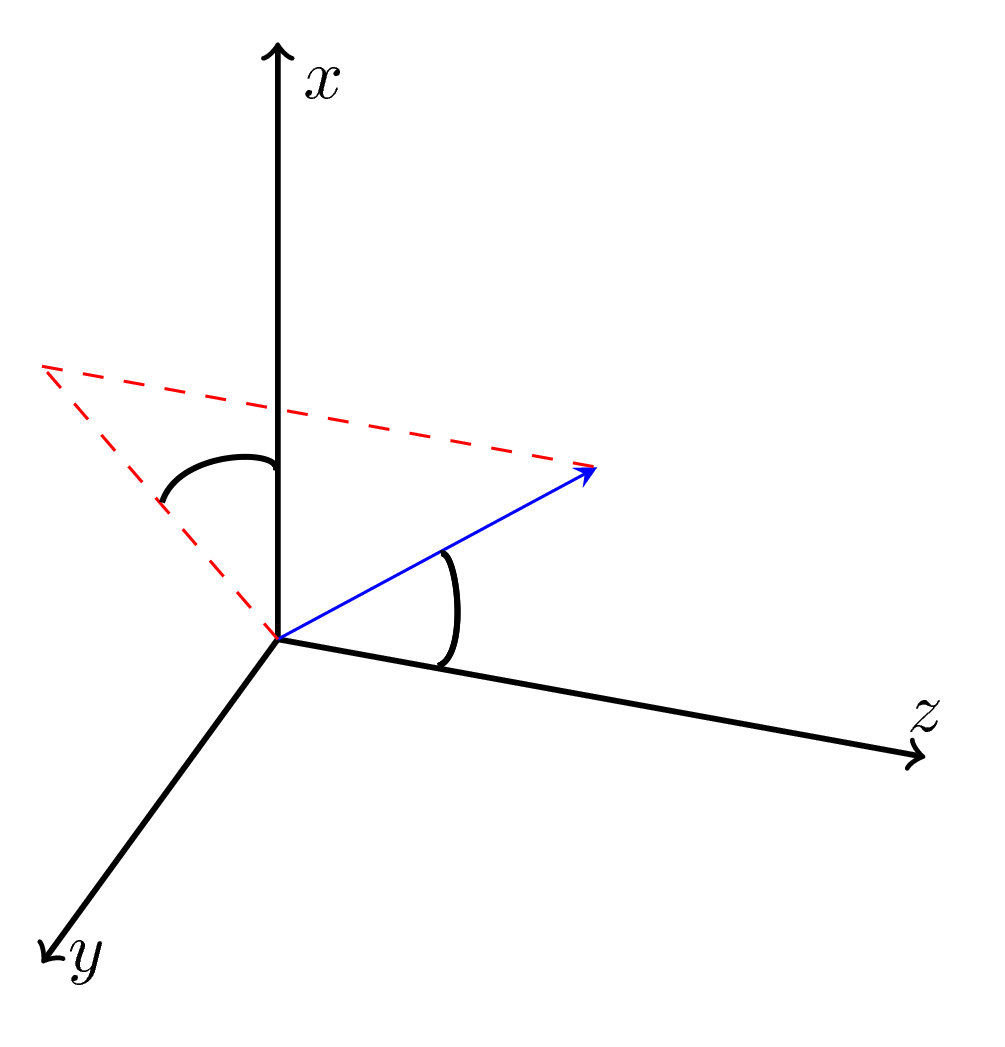
\includegraphics[width=0.2\textheight]{Figures/Geometries/coordinates.png}};
  %   \begin{scope}[x={(image.south east)},y={(image.north west)}]
  %     \node[left, text=black] at (0.27, 0.6){$\phi$};
  %     \node[right, text=black] at (0.45, 0.45){$\theta$};
  %   \end{scope}
  % \end{tikzpicture}
  \tdplotsetmaincoords{60}{120}
  \begin{tikzpicture}
    [scale=3,
      tdplot_main_coords,
      axis/.style={->,black,thick},
      vector/.style={-stealth,ForestGreen,very thick},
      vector guide/.style={dashed,ForestGreen,thick},
      angle/.style={ForestGreen,thick}]
    
    % standard tikz coordinate definition using x, y, z coords
    \coordinate (O) at (0,0,0);
    
    % tikz-3dplot coordinate definition using r, theta, phi coords
    \tdplotsetcoord{P}{.8}{55}{60}
    
    % draw axes
    \draw[axis] (0,0,0) -- (1,0,0) node[anchor=north east]{$x$};
    \draw[axis] (0,0,0) -- (0,1,0) node[anchor=north west]{$y$};
    \draw[axis] (0,0,0) -- (0,0,1) node[anchor=south]{$z$};
    
    % draw a vector from O to P
    \draw[vector] (O) -- (P);
    
    % draw guide lines to components
    \draw[vector guide] (O) -- (Pxy);
    \draw[vector guide] (Pxy) -- (P);
    
    % draw an arc illustrating the angle defining the orientation
    \tdplotdrawarc[angle]{(O)}{.35}{0}{60}{anchor=north}{$\phi$}
    
    % define the rotated coordinate frame to lie in the "theta plane"
    \tdplotsetthetaplanecoords{55}
    
    \tdplotdrawarc[tdplot_rotated_coords,angle]{(O)}{.35}{0}{55}
                  {anchor=south west}{$\theta$}
                  
  \end{tikzpicture}
  \caption{The right-handed coordinate system used to describe the geometry where the beam axis is parallel to the z-axis.}
  \label{fig:coord_system}
\end{figure}
%% \begin{figure}[H]
%%   \centering
%%   % \begin{tikzpicture}
%%   %   \node[anchor=south west,inner sep=0] (image) at (0,0){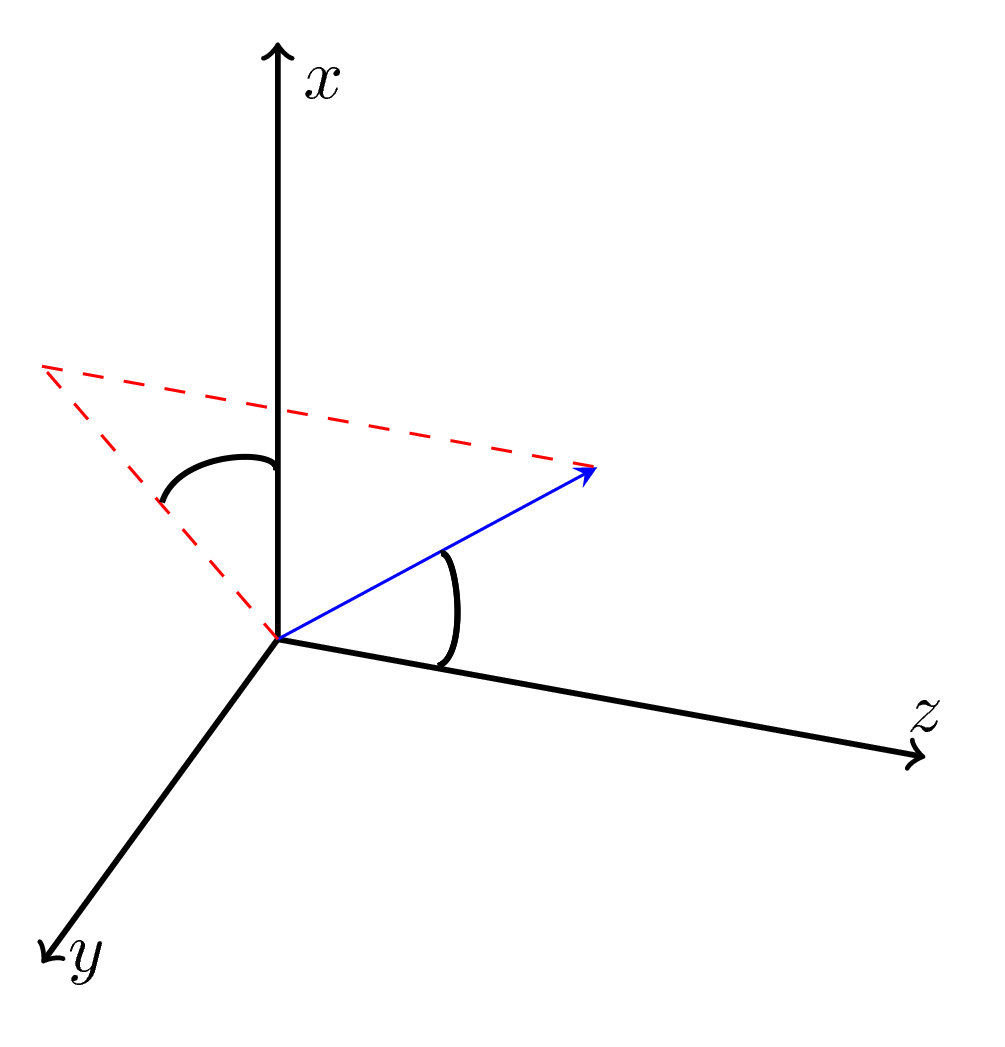
\includegraphics[width=0.2\textheight]{Figures/Geometries/coordinates.png}};
%%   %   \begin{scope}[x={(image.south east)},y={(image.north west)}]
%%   %     \node[left, text=black] at (0.27, 0.6){$\phi$};
%%   %     \node[right, text=black] at (0.45, 0.45){$\theta$};
%%   %   \end{scope}
%%   % \end{tikzpicture}
%%   \begin{tikzpicture}
%%     \node[anchor=south west,inner sep=0] (image) at (0, 0){\includegraphics[trim=80mm 200mm 80mm 50mm, clip, angle=286, width=0.3\textheight]{coord.pdf}};  
%%     \node[] at (2.4, 0.4) {$y$}; 
%%     \node[] at (0.4, 5) {$x$};
%%     \node[] at (5.5, 4.4) {$z$};
%%     \node[color=ForestGreen] at (3.5, 3.5) {$\theta$};
%%     \node[color=ForestGreen] at (1.8, 3.5) {$\phi$};
%%   \end{tikzpicture}
%%   \caption{The coordinate system in which the detector is defined. The beam line is parallel to the z-axis.}
%%   \label{fig:coord_system}
%% \end{figure}
%% \begin{figure}[H]
%%   \centering
%%   % \begin{tikzpicture}
%%   %   \node[anchor=south west,inner sep=0] (image) at (0,0){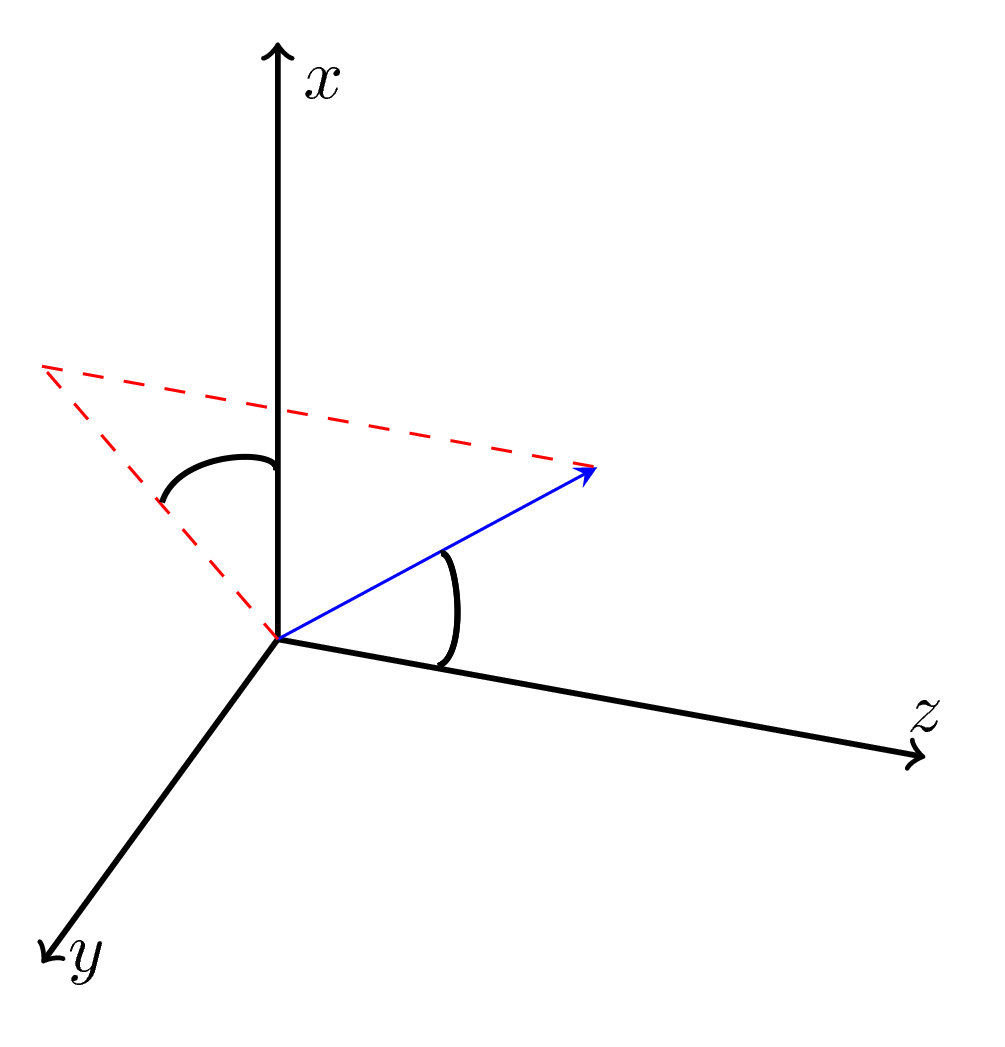
\includegraphics[width=0.2\textheight]{Figures/Geometries/coordinates.png}};
%%   %   \begin{scope}[x={(image.south east)},y={(image.north west)}]
%%   %     \node[left, text=black] at (0.27, 0.6){$\phi$};
%%   %     \node[right, text=black] at (0.45, 0.45){$\theta$};
%%   %   \end{scope}
%%   % \end{tikzpicture}
%%   %% \begin{tikzpicture}
%%   %%   \node[anchor=south west,inner sep=0] (image) at (0, 0){\includegraphics[trim=80mm 200mm 80mm 50mm, clip, angle=286, width=0.3\textheight]{coord.pdf}};  
%%   %%   \node[] at (2.4, 0.4) {$y$}; 
%%   %%   \node[] at (0.4, 5) {$x$};
%%   %%   \node[] at (5.5, 4.4) {$z$};
%%   %%   \node[color=ForestGreen] at (3.5, 3.5) {$\theta$};
%%   %%   \node[color=ForestGreen] at (1.8, 3.5) {$\phi$};
%%   %% \end{tikzpicture}
%%   \caption{The coordinate system in which the detector is defined. The beam line is parallel to the z-axis.}
%%   \label{fig:coord_system}
%% \end{figure}
%----------------------------------------------------------------------
\subsection{The CDR geometry}\label{sec:CLIC_SiD_CDR}
The term "CDR geometry" refers to the CLIC\_SiD geometry as defined in~\cite{CLICCDR2012}. It consists of five concentric layers in the vertex barrel (cf. Figure~\ref{fig:vertex_barrel}) and four disks in the vertex endcaps. 

\begin{figure}[H]
  \centering
  \begin{tikzpicture}
    \node[anchor=south west,inner sep=0] (image) at (0, 0){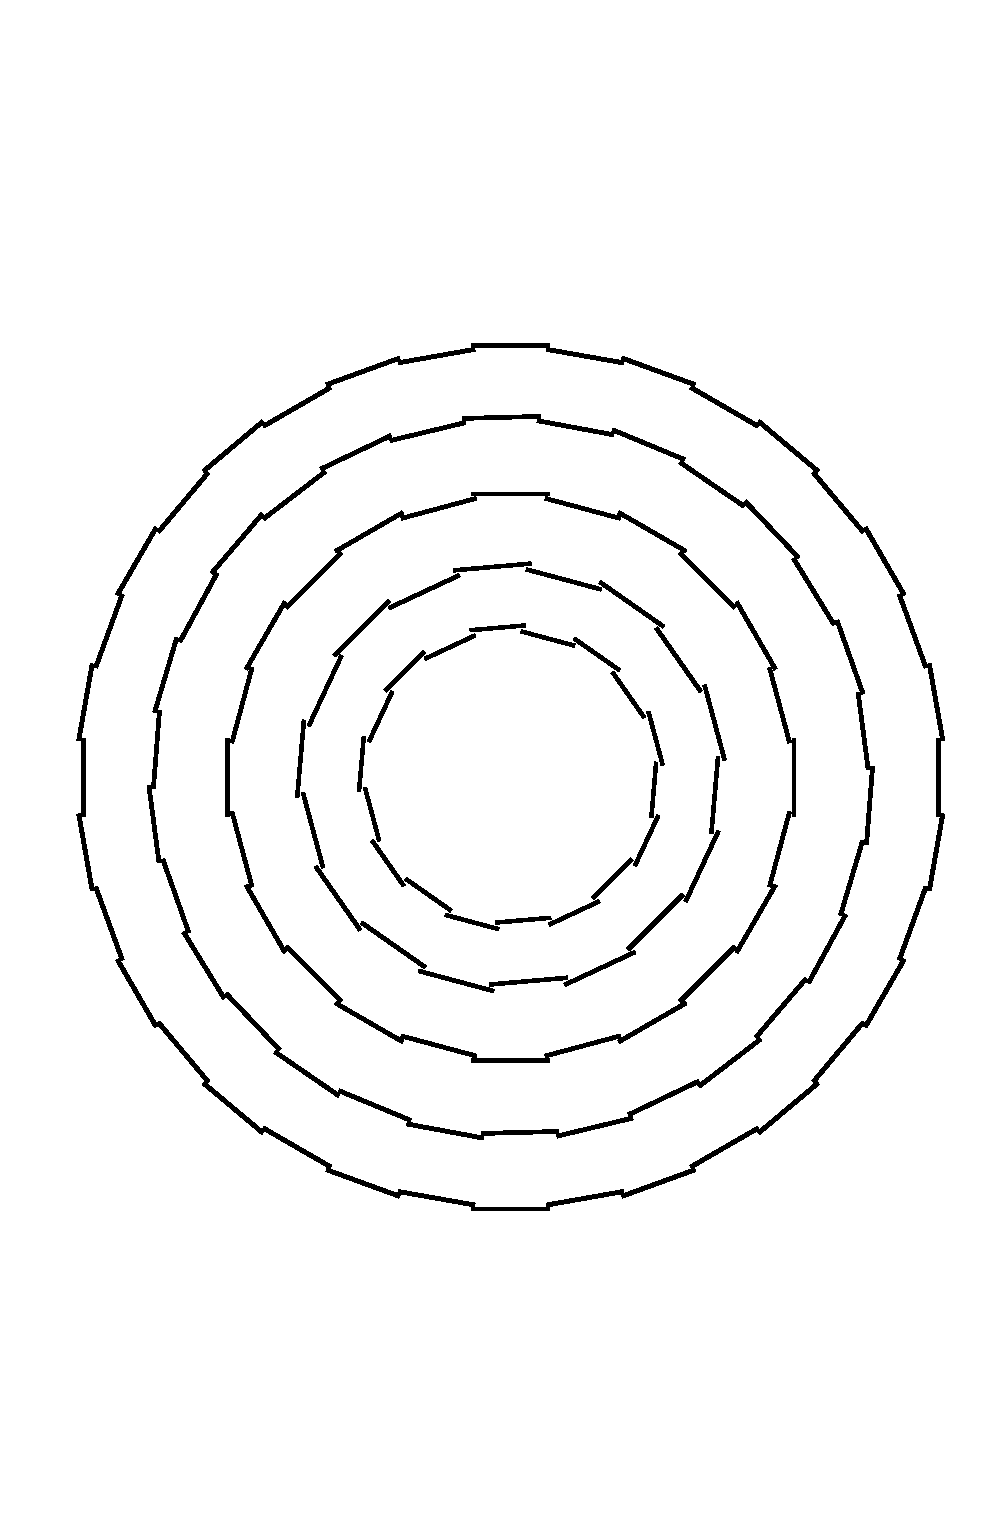
\includegraphics[trim = 0mm 30mm 0mm 30mm, clip,  width=0.3\textheight]{Figures/Geometries/default_barrel.pdf}};
    \draw[->,line width=.4pt, color=ForestGreen](3.6, 4) -- (7.1, 4);
    \node[right, color=ForestGreen] at (7.1, 4) {$x$};
    \draw[->,line width=.4pt, color=ForestGreen](3.6, 4) -- (3.6, 7.5);
    \node[right, color=ForestGreen] at (3.6, 7.5) {$y$};
  \end{tikzpicture}
  \label{fig:vertex_barrel_b}
  \caption{Schematic layout of the vertex barrel detector in the xy-plane for the CDR geometry.}\label{fig:vertex_barrel}
\end{figure}


%% \begin{figure}[H]
%%   \centering
%%   \begin{subfigure}[H]{0.2\textwidth}
%%     \hspace{-5cm}
%%     \vspace{1cm}
%%     
\includegraphics[page=5, trim=0mm 155mm 100mm 50mm, clip, width=0.3\textheight]{Figures/Geometries/LCD-2011-009.pdf}
%%     \caption{}
%%     \label{fig:vertex_barrel_a}
%%   \end{subfigure} \quad
%%   \begin{subfigure}[H]{0.2\textwidth}
%%     \hspace{3cm}
%%     \begin{tikzpicture}
%%       \node[anchor=south west,inner sep=0] (image) at (0, 0){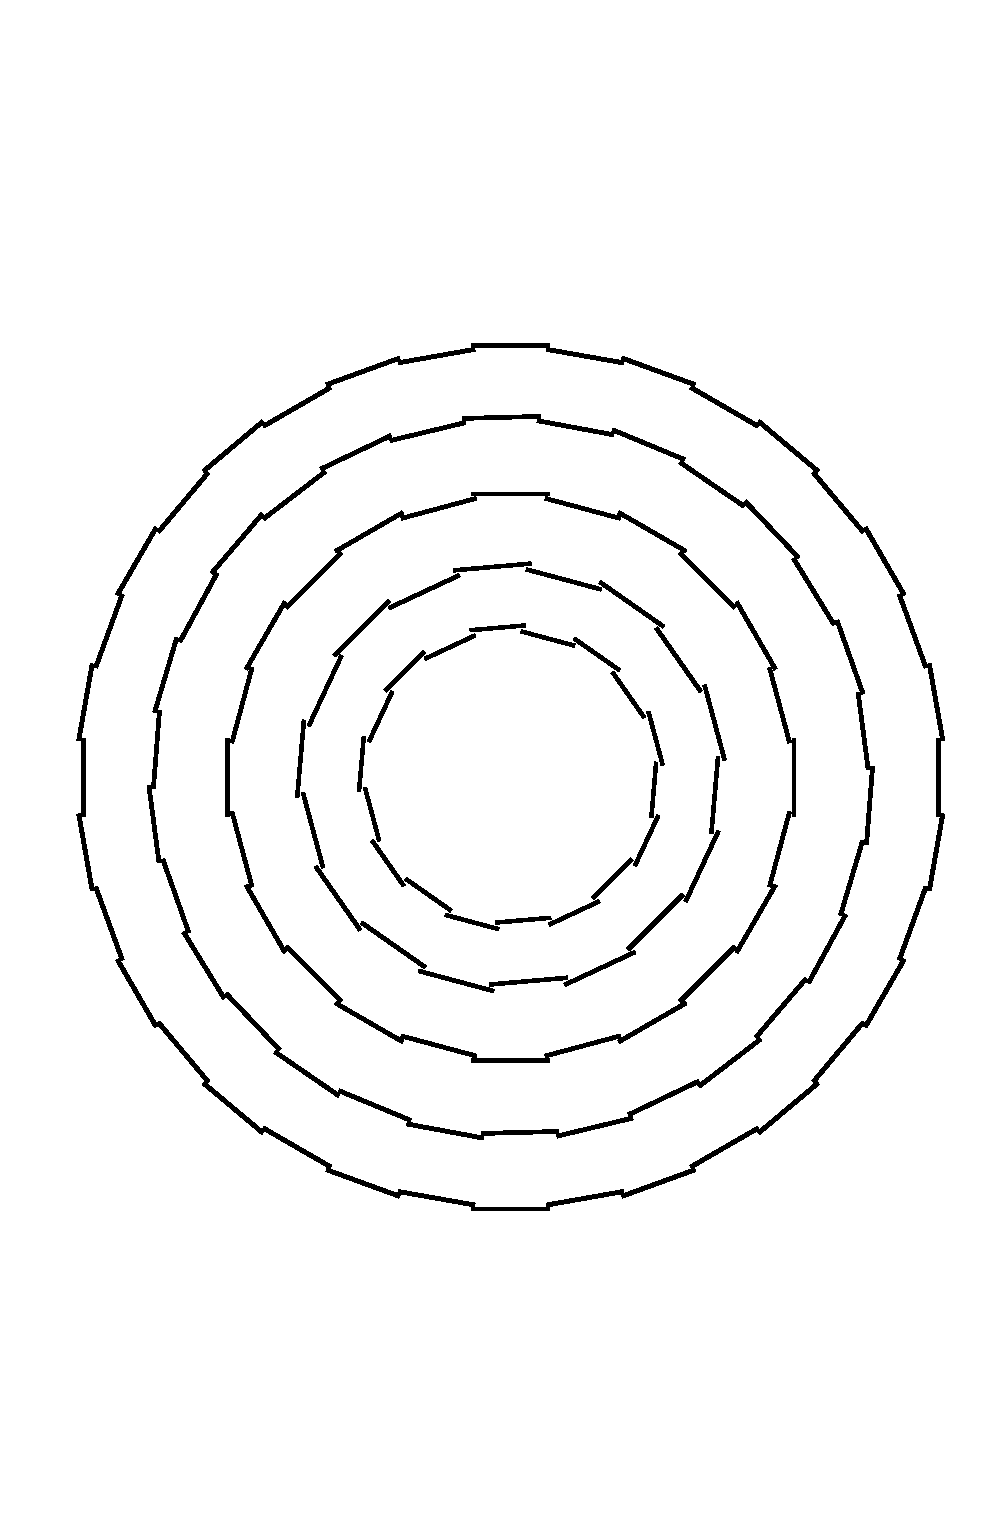
\includegraphics[trim = 0mm 30mm 0mm 30mm, clip,  width=0.3\textheight]{Figures/Geometries/default_barrel.pdf}};
%%       \draw[->,line width=.4pt, color=ForestGreen](3.2, 3.5) -- (6.5, 3.5);
%%       \node[right, color=ForestGreen] at (6.5, 3.5) {$x$};
%%       \draw[->,line width=.4pt, color=ForestGreen](3.2, 3.5) -- (3.2, 6.8);
%%       \node[right, color=ForestGreen] at (3.2, 6.8) {$y$};
%%     \end{tikzpicture}
%%     \caption{}
%%     \label{fig:vertex_barrel_b}
%%   \end{subfigure}
%%   \caption{Schematic layout of the vertex barrel detector in the xy-plane for the CDR geometry. The distances in (a) are given in mm. From~\cite{Grefe2011}.}\label{fig:vertex_barrel}
%% \end{figure}


Each layer in the barrel is composed of several modules as listed in Table~\ref{tab:params_default}. Each module contains a silicon sensor with a thickness of \SI{50}{\micro\meter}. The silicon sensor is the sensitive part of the module which detects the particles passing through it. It is followed by a layer of carbon fiber with a thickness of \SI{130}{\micro\meter}, emulating the material for readout, cabling and supports. The total amount of material per layer corresponds to $0.11\%X_{0}$.\\
 
\begin{table}[H]
  \caption{Parameters for the vertex detector barrel layers for the CDR geometry. \textit{N} represents the number of modules in a layer, \textit{r} the mean radius of the layer, \textit{z} the half-length and \textit{w} the width of the module. In the \textsc{Geant4} simulations, each module consists of \SI{50}{\micro\meter} of silicon followed by \SI{130}{\micro\meter} of carbon fiber. From~\cite{Grefe2011}.}
  \begin{center}
    \begin{tabular}{ c c c c c }
      \hline
      Layer & N & r[mm] & z[mm] & w[mm]\\ \hline \hline
      1 & 18 & 27.0 & 98.5 & 9.8 \\ \hline
      2 & 18 & 38.0 & 98.5 & 13.8 \\ \hline
      3 & 24 & 51.0 & 98.5 & 13.8 \\ \hline
      4 & 30 & 64.0 & 98.5 & 13.8 \\ \hline
      5 & 36 & 77.0 & 98.5 & 13.8 \\ \hline
    \end{tabular}
  \end{center}
  \label{tab:params_default}
\end{table}

The vertex detector contains 4 disks in the endcap regions made of silicon pixel detectors with the parameters given in Table~\ref{tab:params_default_endcap}. Figure~\ref{fig:endcap_placement} shows a schematic layout of the vertex detector with highlighted vertex barrel and endcap. The vertex detector is surrounded by the main tracking system made of silicon strip detectors. 
\begin{figure}[H]
  %\centering
  \hspace{-2cm}
  \begin{tikzpicture}
    \node[anchor=south west,inner sep=0] (image) at (0,0){
\includegraphics[page=6, trim=0mm 210mm 10mm 40mm, clip, width=0.8\textheight]{Figures/Geometries/LCD-2011-009.pdf}};
    \begin{scope}[x={(image.south east)},y={(image.north west)}]
      \draw[Green,ultra thick,rounded corners] (0.15,0.2) rectangle (0.29,0.45);
      \node[above, text=Green] at (0.2, 0.45){Vertex Barrel};
      \draw[Red,ultra thick,rounded corners] (0.295,0.2) rectangle (0.4,0.55);
      \node[above, text=Red] at (0.33, 0.55){Vertex Endcap};
      \draw[->,line width=.4pt, color=ForestGreen](0.9, 0.16) -- (0.95, 0.16);
      \node[right, color=ForestGreen] at (0.95, 0.16) {$z$};
      \draw[->,line width=.4pt, color=ForestGreen](0.9, 0.16) -- (0.9, 0.4);
      \node[right, color=ForestGreen] at (0.9, 0.4) {$y$};
    \end{scope}
  \end{tikzpicture}
  \caption{Schematic layout of the vertex detector in the zy-plane. The distances are given in~mm. From~\cite{Grefe2011}.}
  \label{fig:endcap_placement}
\end{figure}


\begin{table}[H]
  \caption{Parameters for the trapezoidal modules in the forward region
    of the CDR geometry, where \textit{N} represents the number of modules
    in a disk, $r_{in}$ and $r_{out}$ the inner and the outer radius
    for the disks at the outer edge of the trapezoidal modules, $w_{in}$ and $w_{out}$ the inner and the outer
    widths and \textit{z} the position of the modules. In the \textsc{Geant4} simulations, each
    module is made of \SI{50}{\micro\meter} of silicon followed by
    \SI{130}{\micro\meter} of carbon fiber. From~\cite{Grefe2011}.}
  \begin{center}
    \begin{tabular}{ c c c c c c c }
      \hline
      Disk & N & r$_{in}$[mm] & r$_{out}$[mm] & w$_{in}$[mm] & w$_{out}$[mm] & z[mm] \\ \hline \hline
      1 & 16 & 27.0 & 115.0 & 10.8 & 45.1 & 120.0 \\ \hline
      2 & 16 & 27.0 & 115.0 & 10.8 & 45.1 & 160.0 \\ \hline
      3 & 16 & 27.0 & 115.0 & 10.8 & 45.1 & 200.0 \\ \hline
      4 & 16 & 28.1 & 115.0 & 11.3 & 45.1 & 240.0\\ \hline
    \end{tabular}
  \end{center}
  \label{tab:params_default_endcap}
\end{table}

%% The vertex detector is designed to provide excellent point resolution with low material budget in order to minimize multiple scattering in the detector. 
Figure~\ref{fig:default_nb_barrel_endcap} shows the angular coverage of the vertex barrel and the vertex endcaps separately. The vertex detector can measure tracks down to a polar angle of about $\theta = 8^\circ$. The number of measured points affects the performance of the particle track reconstruction. 

\begin{figure}[H]
  \centering
  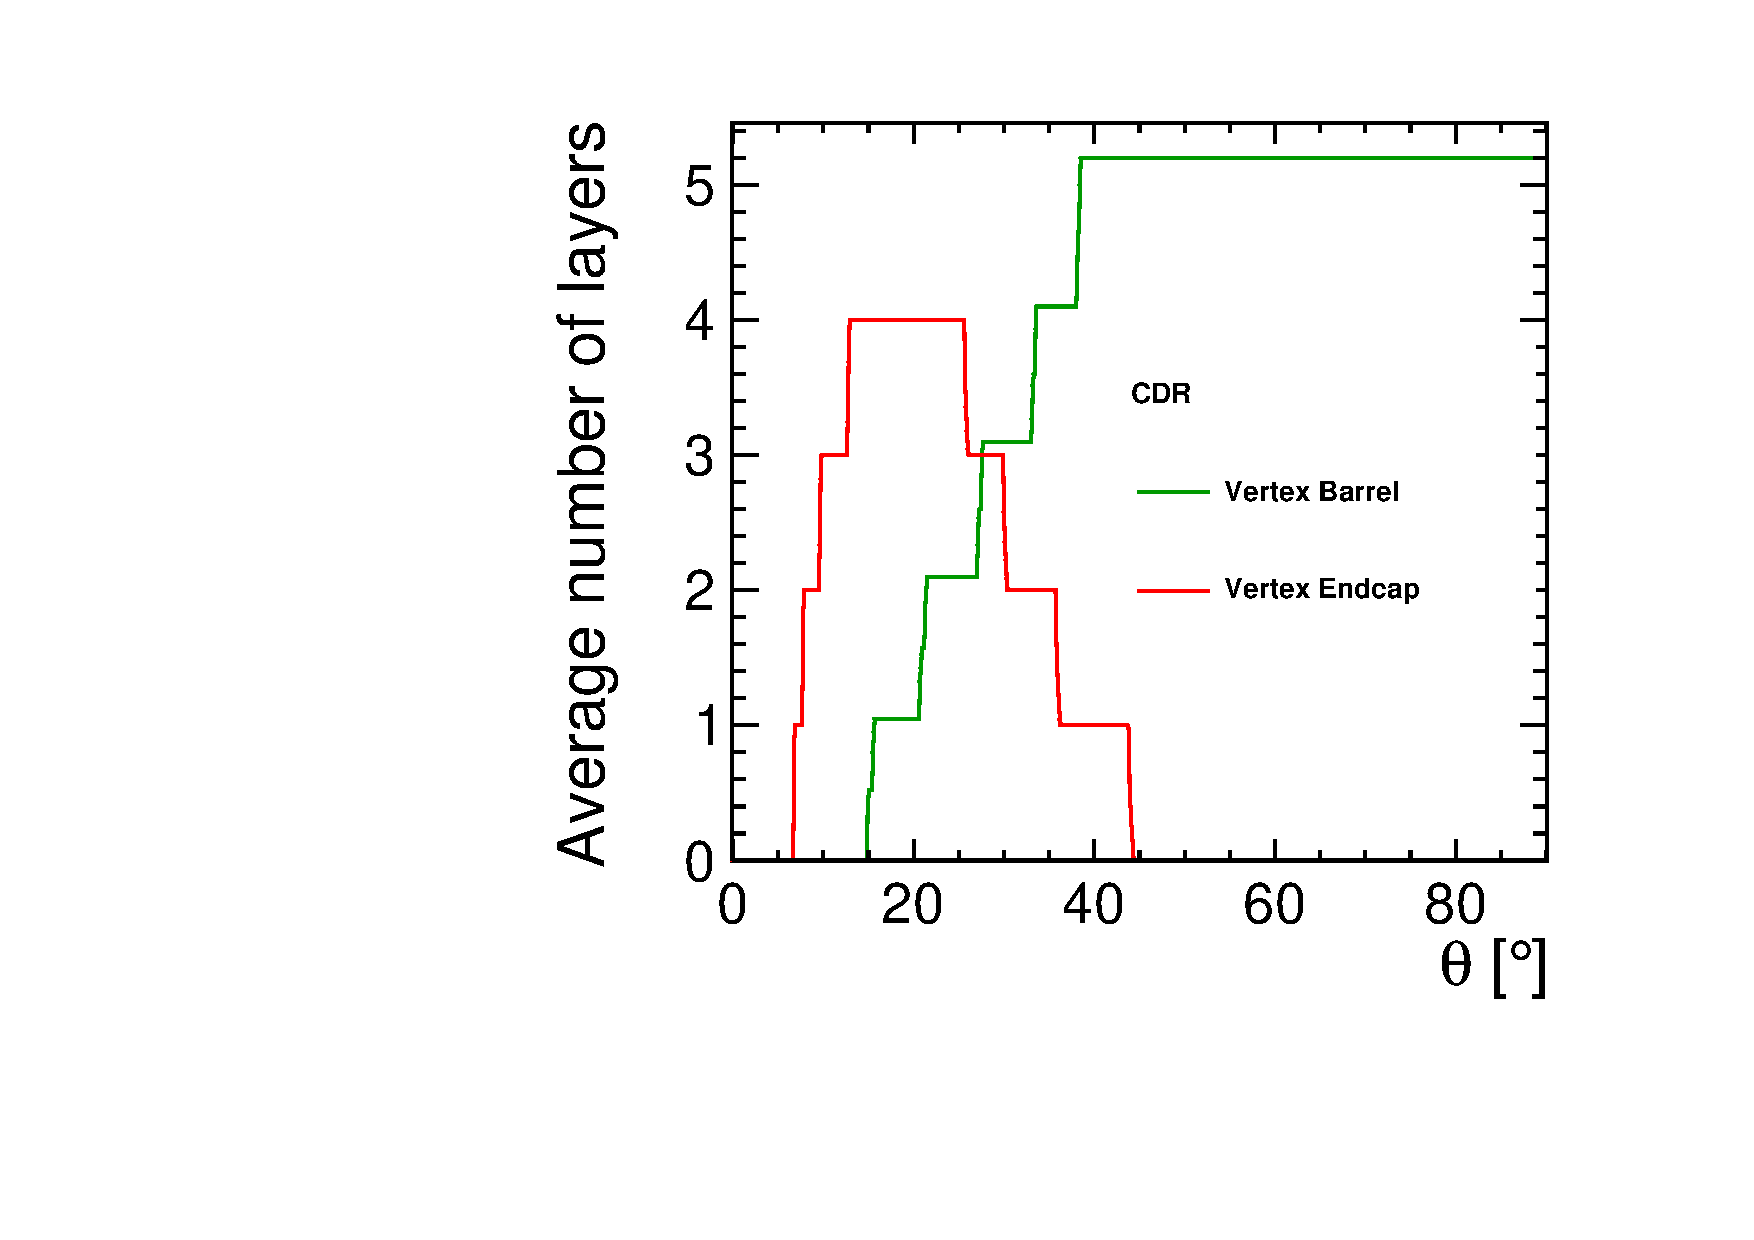
\includegraphics[scale=0.4]{Figures/Geometries/nb_layer_cdr.pdf}
  \caption{The coverage of the vertex detector with respect to the polar angle $\theta$ for the CDR geometry. The number of layers is averaged over the azimuthal angle $\phi$.}
  \label{fig:default_nb_barrel_endcap}
\end{figure}

%----------------------------------------------------------------------
\subsection{The \emph{spirals} geometry}\label{sec:CLIC_SiD_spirals}

Several engineering studies are in progress to limit the material, e.g. the cables, the mechanical support and also the cooling. Cooling solutions with pipes and liquids increase significantly the material budget. The aim is therefore to use airflow cooling for the CLIC vertex detector. \\
However, the CDR geometry was not designed for the airflow cooling. The vertex endcaps, which are made of disks, do not allow the air to flow through the vertex detector. \\
One solution is to use a spiral arrangement for the modules in the endcap regions~\cite{CoolingSimulations}. Figure~\ref{fig:spirals_cooling_simulations} illustrates the airflow cooling concept for the vertex detector. The air can flow through the endcap on one side, continue along the barrel sensors and flow out through the other endcap.

%% \begin{figure}[H]
%%   \centering
%%   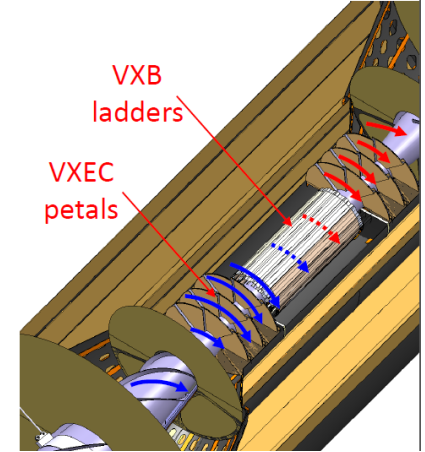
\includegraphics[scale=0.3]{Figures/Geometries/airflow.png}
%%   \caption{Engineering model for the vertex detector with spiral endcap disks: the air flows into the endcap on one side and out from the other endcap passing the barrel region.}\label{fig:spirals_cooling_simulations}
%% \end{figure}

\begin{figure}[H]
  \centering
  \includegraphics[page=8, trim = 20mm 85mm 20mm 155mm, clip, width=\textwidth]{Figures/LCD-Note-cooling.pdf}
  \caption{Engineering sketch showing the airflow cooling strategy within the vertex detector. From~\cite{CoolingSimulations}.}\label{fig:spirals_cooling_simulations}
\end{figure}

The parameters for the spiral arrangement of the sensors in the vertex endcaps are given in Table~\ref{tab:params_spiral_endcap}. For this geometry the number of trapezoidal modules \textit{N} in a layer is reduced to 8 compared to 16 for the CDR geometry. In Table~\ref{tab:params_spiral_endcap}, \textit{z} gives the distance of the first module of each layer to the interaction point in the vertex endcaps and the modules are interspaced by a distance of $\Delta z$=3.6~mm. The first module in each layer covers the azimuthal angle from $\phi=157.5^{\circ}$ to $\phi=202.5^{\circ}$.\\
Figure~\ref{fig:singleSpiralGeom} shows the \begin{it}spirals\end{it} geometry as implemented in the simulations. The barrel geometry is identical to the one of the CDR geometry. 

\begin{table}[H]
  \caption{Parameters for the trapezoidal modules in the endcap regions
    of the {\it spirals} geometry, where \textit{N} represents the
    number of modules in a layer, $r_{in}$ and $r_{out}$ the inner and
    the outer radius at the outer edge of the trapezoidal modules,
    $w_{in}$ and $w_{out}$ the inner and the outer widths, \textit{z}
    the position of the first module of the layer. The other modules are placed at a distance of $\Delta$\textit{z}=3.6~mm from the previous module in the \textit{z} direction. In the \textsc{Geant4} simulations, each module is made of \SI{50}{\micro\meter} of silicon followed by \SI{130}{\micro\meter} of carbon fiber.}
  \begin{center}
    \begin{tabular}{ c c c c c c c }
      \hline
      Layer & N & r$_{in}$[mm] & r$_{out}$[mm] & w$_{in}$[mm] & w$_{out}$[mm] & z[mm] \\ \hline \hline
      1 & 8 & 27.0 & 115.0 & 22.7 & 96.6 & 120.0 \\ \hline
      2 & 8 & 27.0 & 115.0 & 22.7 & 96.6 & 150.0 \\ \hline
      3 & 8 & 27.0 & 115.0 & 22.7 & 96.6 & 180.0 \\ \hline
      4 & 8 & 28.1 & 115.0 & 23.6 & 96.6 & 210.0\\ \hline
    \end{tabular}
  \end{center}
  \label{tab:params_spiral_endcap}
\end{table}

\begin{figure}[H]
  \centering
  \begin{tikzpicture}
    \node[anchor=south west,inner sep=0] (image) at (0,0){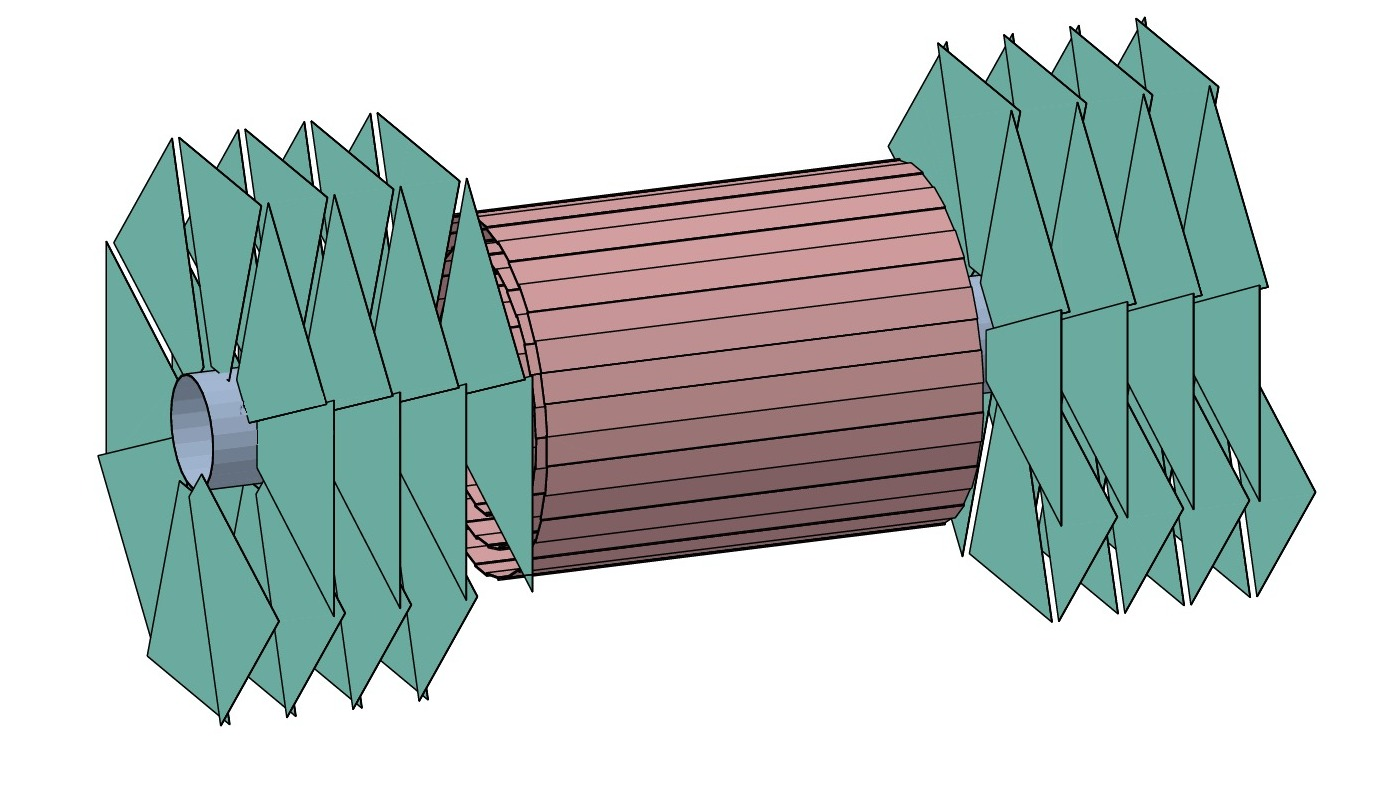
\includegraphics[width=15cm]{Figures/Geometries/single_spiral.jpg}};
    \draw[->,line width=.4pt, color=ForestGreen](15, 5) -- (15, 7);
    \node[right, color=ForestGreen] at (15, 7) {$y$};
    \draw[->,line width=.4pt, color=ForestGreen](15, 5) -- (16.6, 5.2);
    \node[right, color=ForestGreen] at (16.6, 5.2) {$z$};
    \draw[->,line width=.4pt, color=ForestGreen](15, 5) -- (13.7, 5.6);
    \node[right, color=ForestGreen] at (13.7, 5.6) {$x$};
  \end{tikzpicture}
  \caption{Schematic view of the vertex detector for the {\it spirals} geometry. The barrel is shown in red and is the same as the CDR barrel. The vertex endcaps modules are shown in green.}
  \label{fig:singleSpiralGeom}
\end{figure}

To minimise the effect of multiple scattering, a low material budget is required for the vertex detector. Figure~\ref{fig:materialBudgSpiralEndcap} compares the material budget for the CDR and the \begin{it}spirals\end{it} geometries. For the computation of the material budget we integrate from the interaction point to the outside of the highlighted areas in Figure~\ref{fig:endcap_placement}, including the beam pipe and cabling. For each polar angle $\theta$, the material budget is averaged over the azimuthal angle $\phi$. As shown in Figure~\ref{fig:materialBudgSpiralEndcap}, the amount of material does not differ much for the \begin{it}spirals\end{it} geometry compared to the CDR layout (the large peak at low polar angles corresponds to the beam pipe).  \\
The number of silicon layers as a function of the polar angles $\theta$ averaged over $\phi$ is given in Figure~\ref{fig:spiral_nb_barrel_endcap} and is very similar for the CDR and the \begin{it}spirals\end{it} geometries. The main difference compared to the disks (see Figure~\ref{fig:default_nb_barrel_endcap}) is that the number of layers varies with the $\phi$ angle.


\begin{figure}[H]
  \begin{subfigure}[b]{0.5\textwidth}
    \centering
    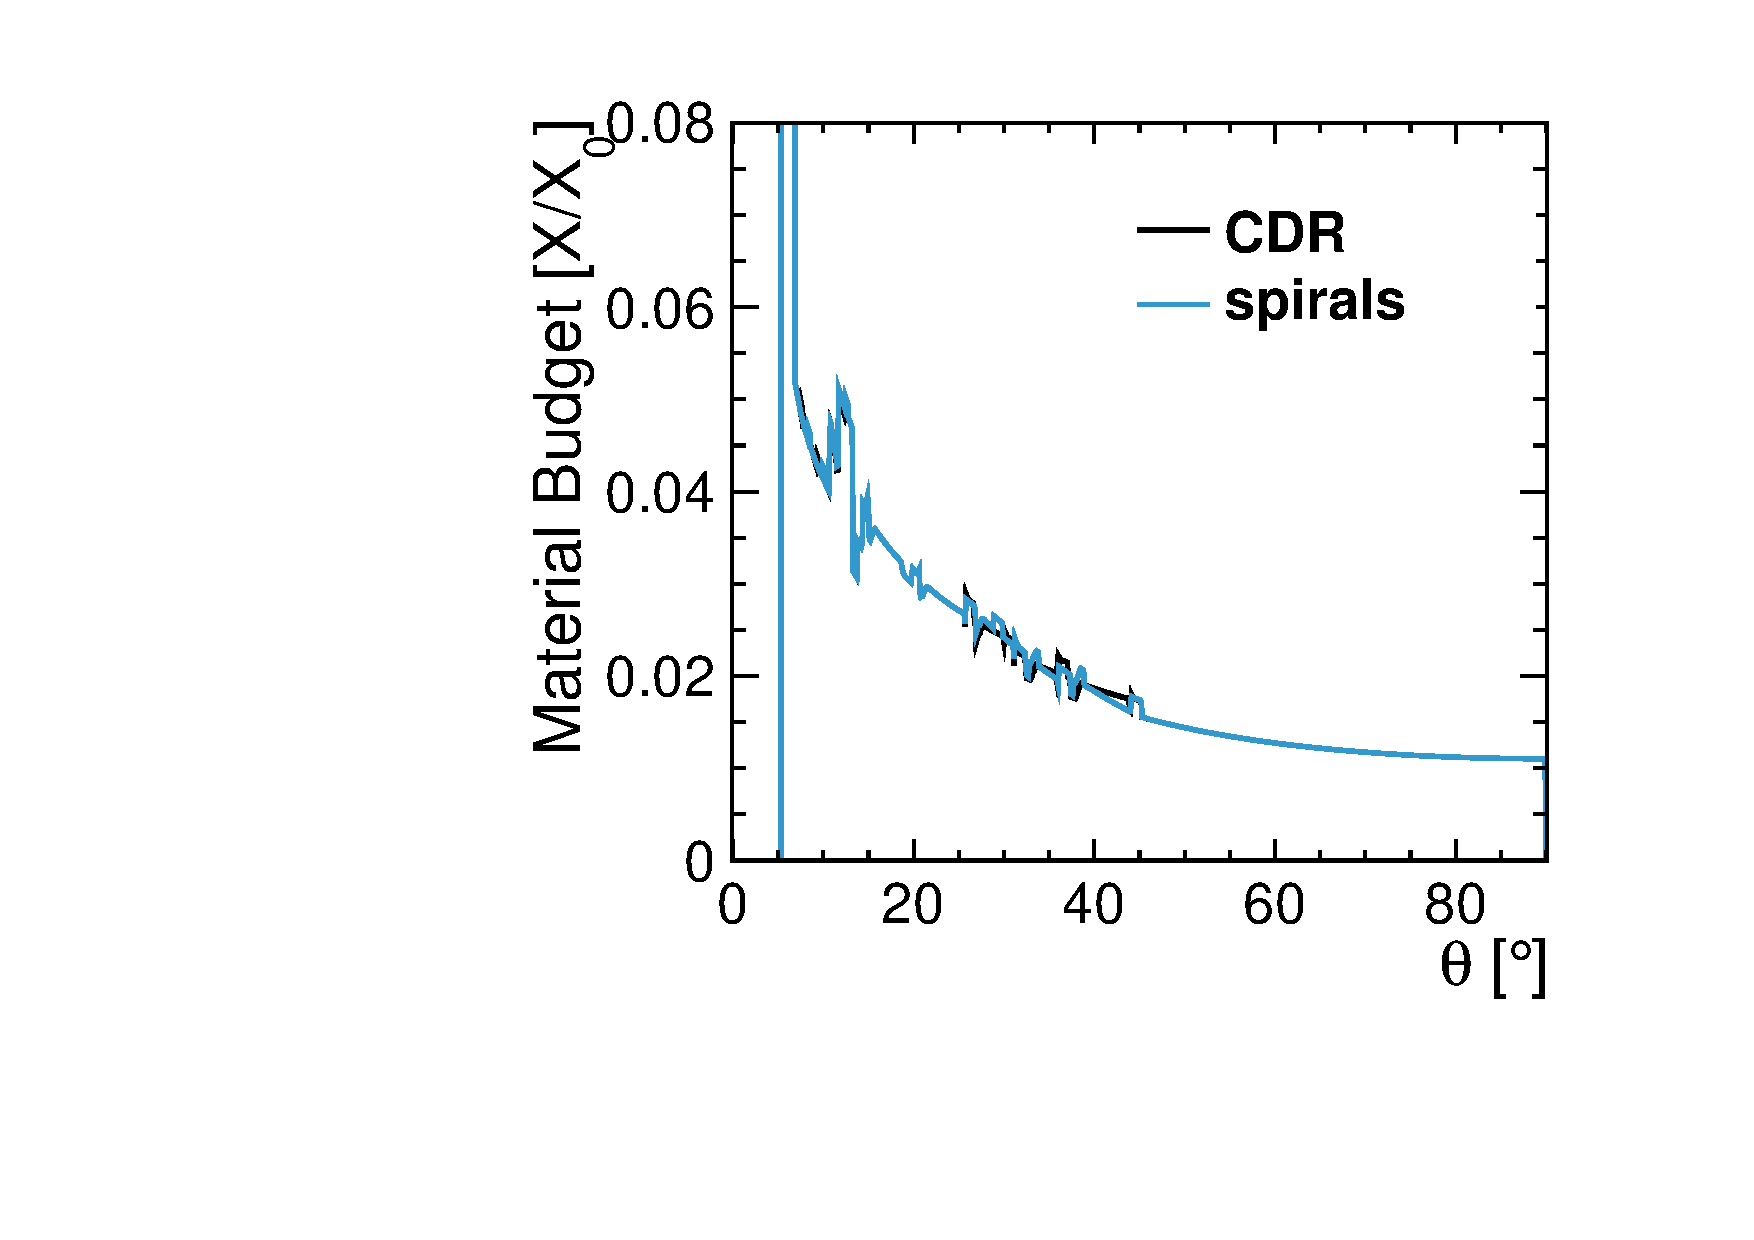
\includegraphics[scale=0.4]{Figures/Geometries/material_budget_spirals.pdf}
    \caption{}\label{fig:materialBudgSpiralEndcap}
  \end{subfigure}~
  \begin{subfigure}[b]{0.5\textwidth}
    \centering
    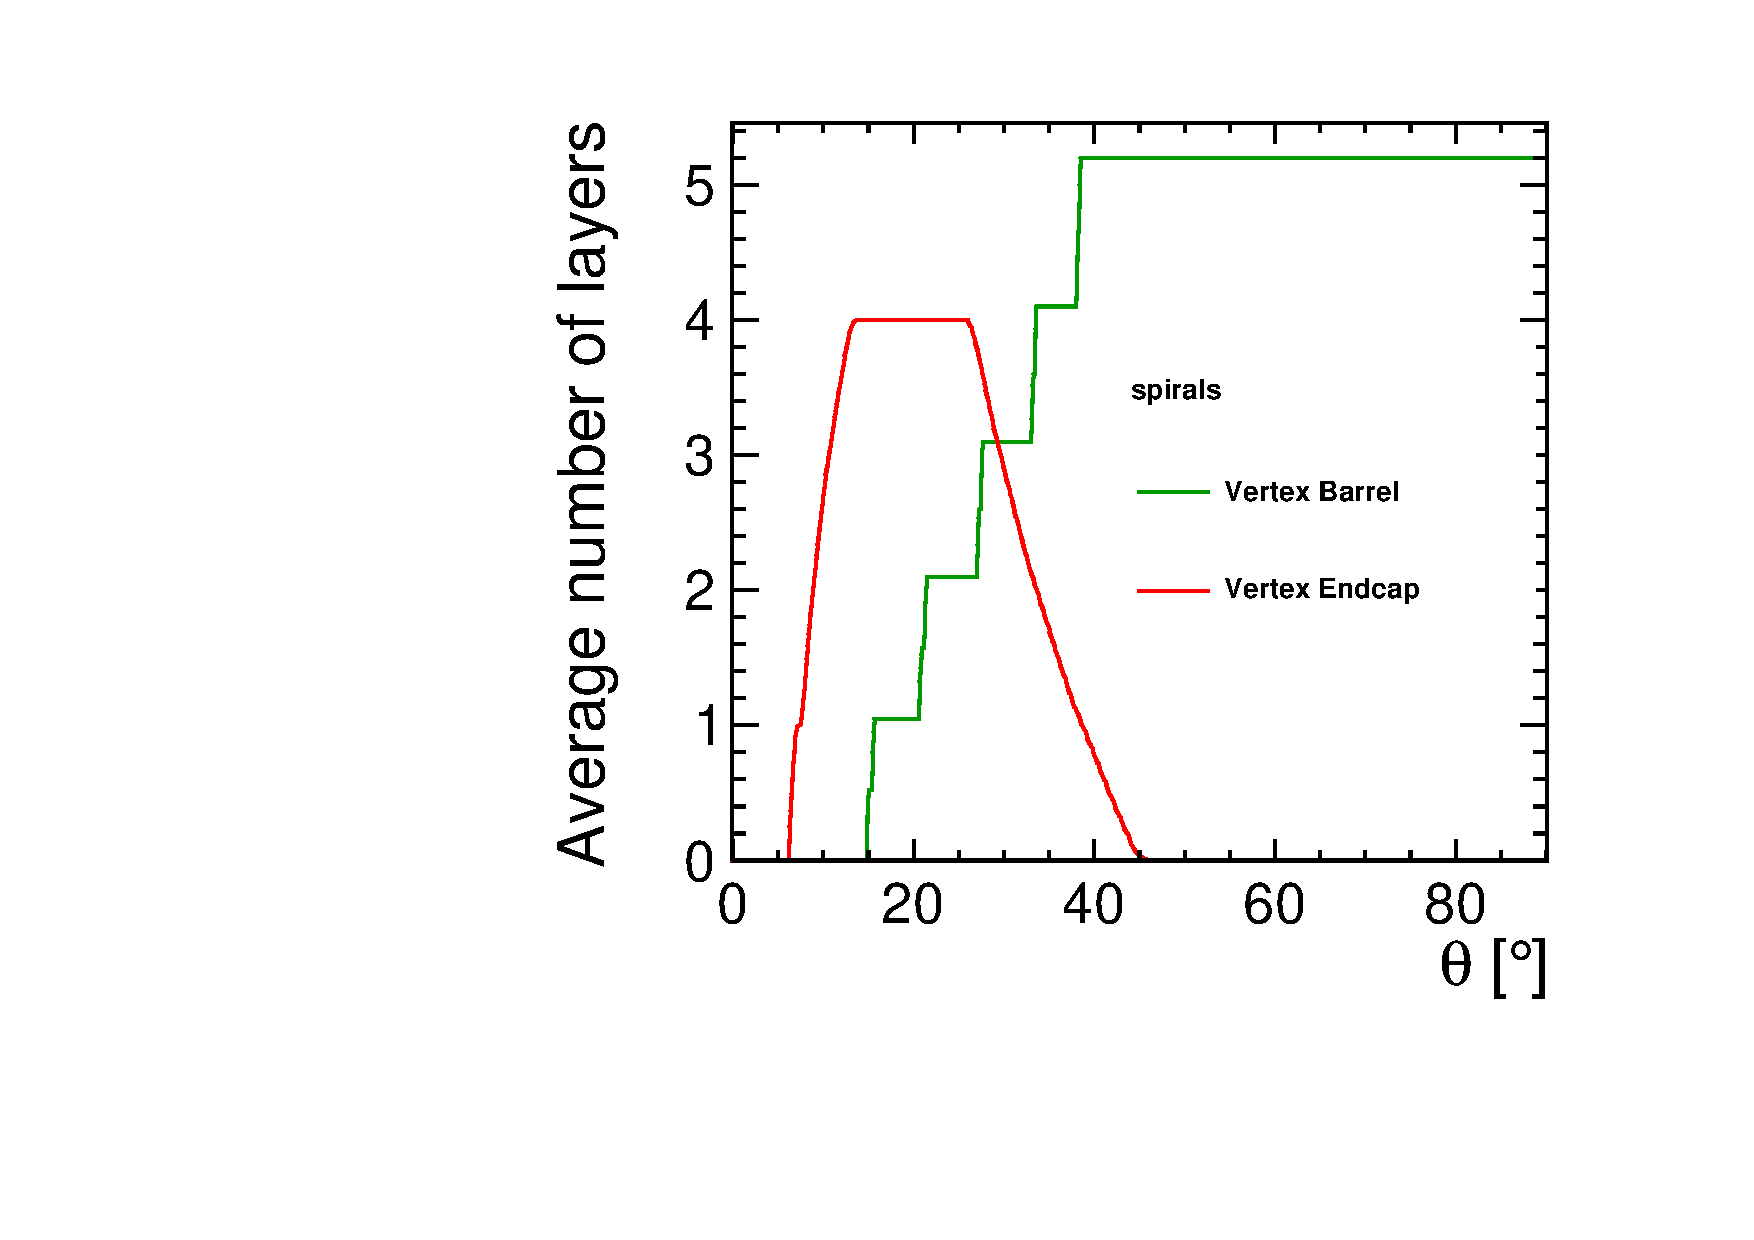
\includegraphics[scale=0.4]{Figures/Geometries/nb_layer_spirals.pdf}
    \caption{}\label{fig:spiral_nb_barrel_endcap}
  \end{subfigure}
  \caption{The material budget for the CDR and the {\it spirals} vertex detectors is shown in (a). The coverage of the vertex detector for the {\it spirals} geometry with respect to the polar angle $\theta$ is shown in (b). The material budget and the number of layers for each polar angle $\theta$ are averaged over the azimuthal angle $\phi$.}
\end{figure}


%----------------------------------------------------------------------
\subsection{The \emph{double\_spirals} geometry}\label{sec:CLIC_SiD_double_spirals}

In the vertex detector, we would like to have as many measurement points as possible and, at the same time, minimise the amount of material. The \begin{it}double\_spirals\end{it} geometry uses two silicon sensors on either side of a single mechanical support in the barrel and the endcap regions. As airflow is foreseen for the heat removal of the detector, a spiral arrangement of the modules is used in the endcap regions as in Section~\ref{sec:CLIC_SiD_spirals}. \\
In the barrel region, the five layers of single-sided modules are replaced by three layers of double-sided modules. Similarly, in the vertex endcaps, instead of four single layers, there are three double layers in a spiral arrangement.\\
Both sides of each module contain silicon sensors with a thickness of \SI{50}{\micro\meter} (cf. Figure~\ref{fig:DL_vertex_barrel_b}). The overall thickness of the carbon fiber used to emulate the mechanical support, cabling and the electronics is \SI{130}{\micro\meter} (each silicon sensor is followed by \SI{65}{\micro\meter} carbon fiber support) and the rest of the module is filled with air. The overall thickness of a double-layer module is \SI{2}{\milli\meter} and is based on the CLIC\_ILD\_CDR layout~\cite{Muennich:1443543} with a material budget of $0.18\%X_{0}$. A schematic view of the double-layered sensor as implemented in the simulations is shown in Figure~\ref{fig:DL_vertex_barrel}. The thickness of the carbon per module layer is the same as the one used for the CDR geometry as we assume that the same amount of support structure and cables is used for the single and the double-layered sensors. The parameters of the \begin{it}double\_spirals\end{it} geometry are given in Tables \ref{tab:params_DL} and \ref{tab:params_double_endcap}.
Figure~\ref{fig:doubleSpiralGeom} illustrates the vertex detector
implemented with double-layered sensors.
\begin{table}[H]
  \caption{Parameters of the vertex barrel layers for the {\it
      double\_spirals} geometry, where \textit{N} represents the
    number of modules in a layer, \textit{r} is the mean radius of the
    layer, \textit{z} the half-length of the module and \textit{w} is
    the width of the module. Each module is made of two layers of
    silicon sensors with a thickness of \SI{50}{\micro\meter} plus \SI{65}{\micro\meter} of carbon fiber.}
  \label{tab:params_DL}
  \begin{center}
    \begin{tabular}{ c c c c c }
      \hline
      Layer & N & r[mm] & z[mm] & w[mm]\\ \hline \hline
      1 & 18 & 27.0 & 98.5 & 9.8 \\ \hline
      2 & 24 & 51.0 & 98.5 & 13.8 \\ \hline
      3 & 36 & 77.0 & 98.5 & 13.8 \\ \hline
    \end{tabular}
  \end{center}  
\end{table}

\begin{table}[H]
  \caption{Parameters for the trapezoidal modules of the {\it
      double\_spirals} geometry in the endcap regions, where
    \textit{N} represents the number of modules in a layer, $r_{in}$
    and $r_{out}$ the inner and the outer radius for the disks at the
    outer edge of the trapezoidal modules, \textit{z} the position of
    the first module of the layer. The other modules are placed at a
    distance of $\Delta z$=5~mm from the previous module in the
    \textit{z} direction. For the trapezoidal modules, $w_{in}$ and
    $w_{out}$ represent the inner and the outer widths. Each module is
    made of two layers of silicon sensors with a thickness of
    \SI{50}{\micro\meter} plus \SI{65}{\micro\meter} of carbon fiber.}
  \begin{center}
    \begin{tabular}{ c c c c c c c }
      \hline
      Layer & N & r$_{in}$[mm] & r$_{out}$[mm] & w$_{in}$[mm] & w$_{out}$[mm] & z[mm] \\ \hline \hline
      1 & 8 & 27.0 & 115.0 & 22.7 & 96.6 & 120.0 \\ \hline
      2 & 8 & 27.0 & 115.0 & 22.7 & 96.6 & 160.0 \\ \hline
      3 & 8 & 27.0 & 115.0 & 22.7 & 96.6 & 200.0 \\ \hline
    \end{tabular}
  \end{center}
  \label{tab:params_double_endcap}
\end{table}

\vspace{-0.2cm}

\begin{figure}[H]
  \begin{subfigure}[]{0.5\textwidth}
    \centering
    
\includegraphics[trim = 0mm 30mm 0mm 30mm, clip, width=7cm]{Figures/Geometries/double_barrel_module.pdf}\caption{}\label{fig:DL_vertex_barrel_a}
  \end{subfigure}~
  \begin{subfigure}[c]{0.5\textwidth}
    \vspace{6.5cm}
    
\includegraphics[width=\textwidth]{Figures/Geometries/double_layer_module.png}\caption{}\label{fig:DL_vertex_barrel_b}
    % \vspace{-2cm}
    % \begin{tikzpicture}
    %   \node[anchor=south west,inner sep=0] at (0,0){
\includegraphics[trim = 75mm 50mm 73mm 200mm, clip, width=7cm]{Figures/Geometries/double_barrel_module.pdf}};
    %   \draw[<->,line width=.4pt, red, thick](3.5,0.2) to node[midway, xshift=0.7cm, red]{2 mm} (3.5,0.86);
    % \end{tikzpicture}
    % \label{fig:DLzoom_vertex_barrel}
  \end{subfigure}
    \caption{The schematic view of the vertex barrel of the {\it double\_spirals} geometry is shown in (a). In the \textsc{Geant4} simulations, each module is implemented as two silicon sensors on top of each other and the overall thickness of the module is \SI{2}{\milli\meter} as illustrated in (b). }\label{fig:DL_vertex_barrel}
\end{figure}

\begin{figure}[H]
  \centering
  \begin{tikzpicture}
    \node[anchor=south west,inner sep=0] (image) at (0,0){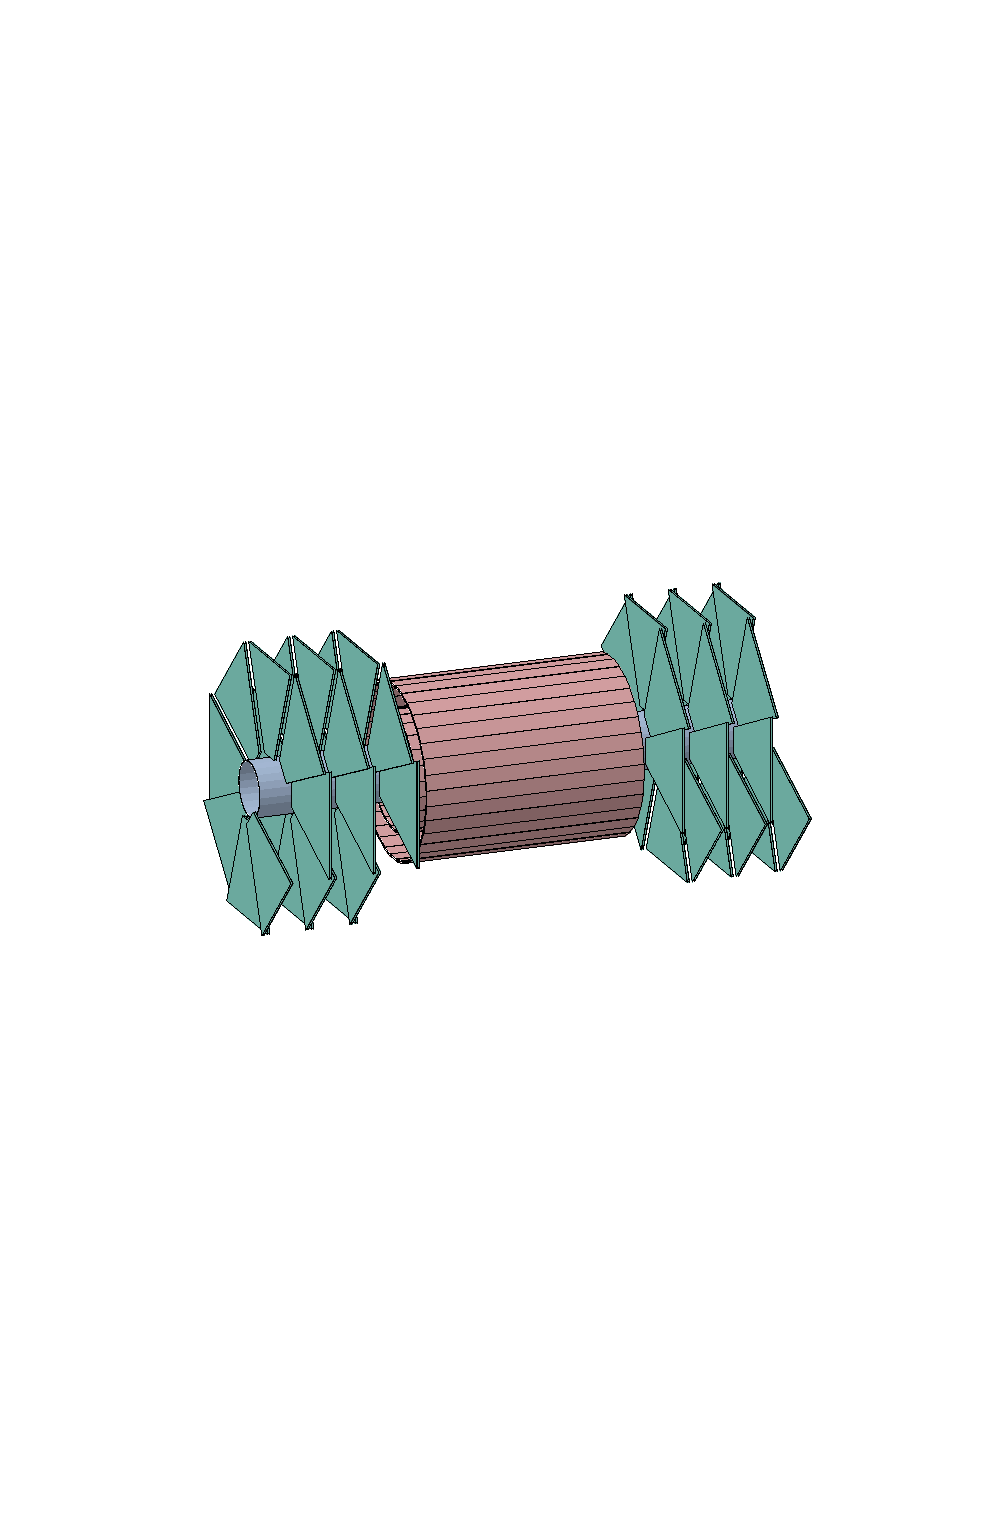
\includegraphics[trim = 20mm 98mm 20mm 90mm, clip, width=15cm]{Figures/Geometries/double_spiral.pdf}};
    \draw[->,line width=.4pt, color=ForestGreen](15, 5) -- (15, 7);
    \node[right, color=ForestGreen] at (15, 7) {$y$};
    \draw[->,line width=.4pt, color=ForestGreen](15, 5) -- (16.6, 5.2);
    \node[right, color=ForestGreen] at (16.6, 5.2) {$z$};
    \draw[->,line width=.4pt, color=ForestGreen](15, 5) -- (13.7, 5.6);
    \node[left, color=ForestGreen] at (13.7, 5.6) {$x$};
  \end{tikzpicture}
  \caption{Schematic view of the vertex detector for the {\it double\_spirals} geometry. The barrel region is shown in red and the vertex endcaps in green.}
  \label{fig:doubleSpiralGeom}
\end{figure}

The material budget for the {\it double\_spirals} geometry is shown in Figure~\ref{fig:materialBudgSpiralEndcap_double} and is very similar to the CDR geometry. The amount of silicon layers has increased but overall less carbon is needed for the mechanical support. \\
Figure~\ref{fig:double_nb_barrel_endcap} shows the coverage of the {\it double\_spirals} geometry. The average number of layers in the vertex endcaps is higher than for the CDR and the \begin{it}spirals\end{it} geometries with similar material budget (see Figures \ref{fig:default_nb_barrel_endcap} and \ref{fig:spiral_nb_barrel_endcap}). 

\begin{figure}[H]
  \begin{subfigure}[b]{0.5\textwidth}
    \centering
    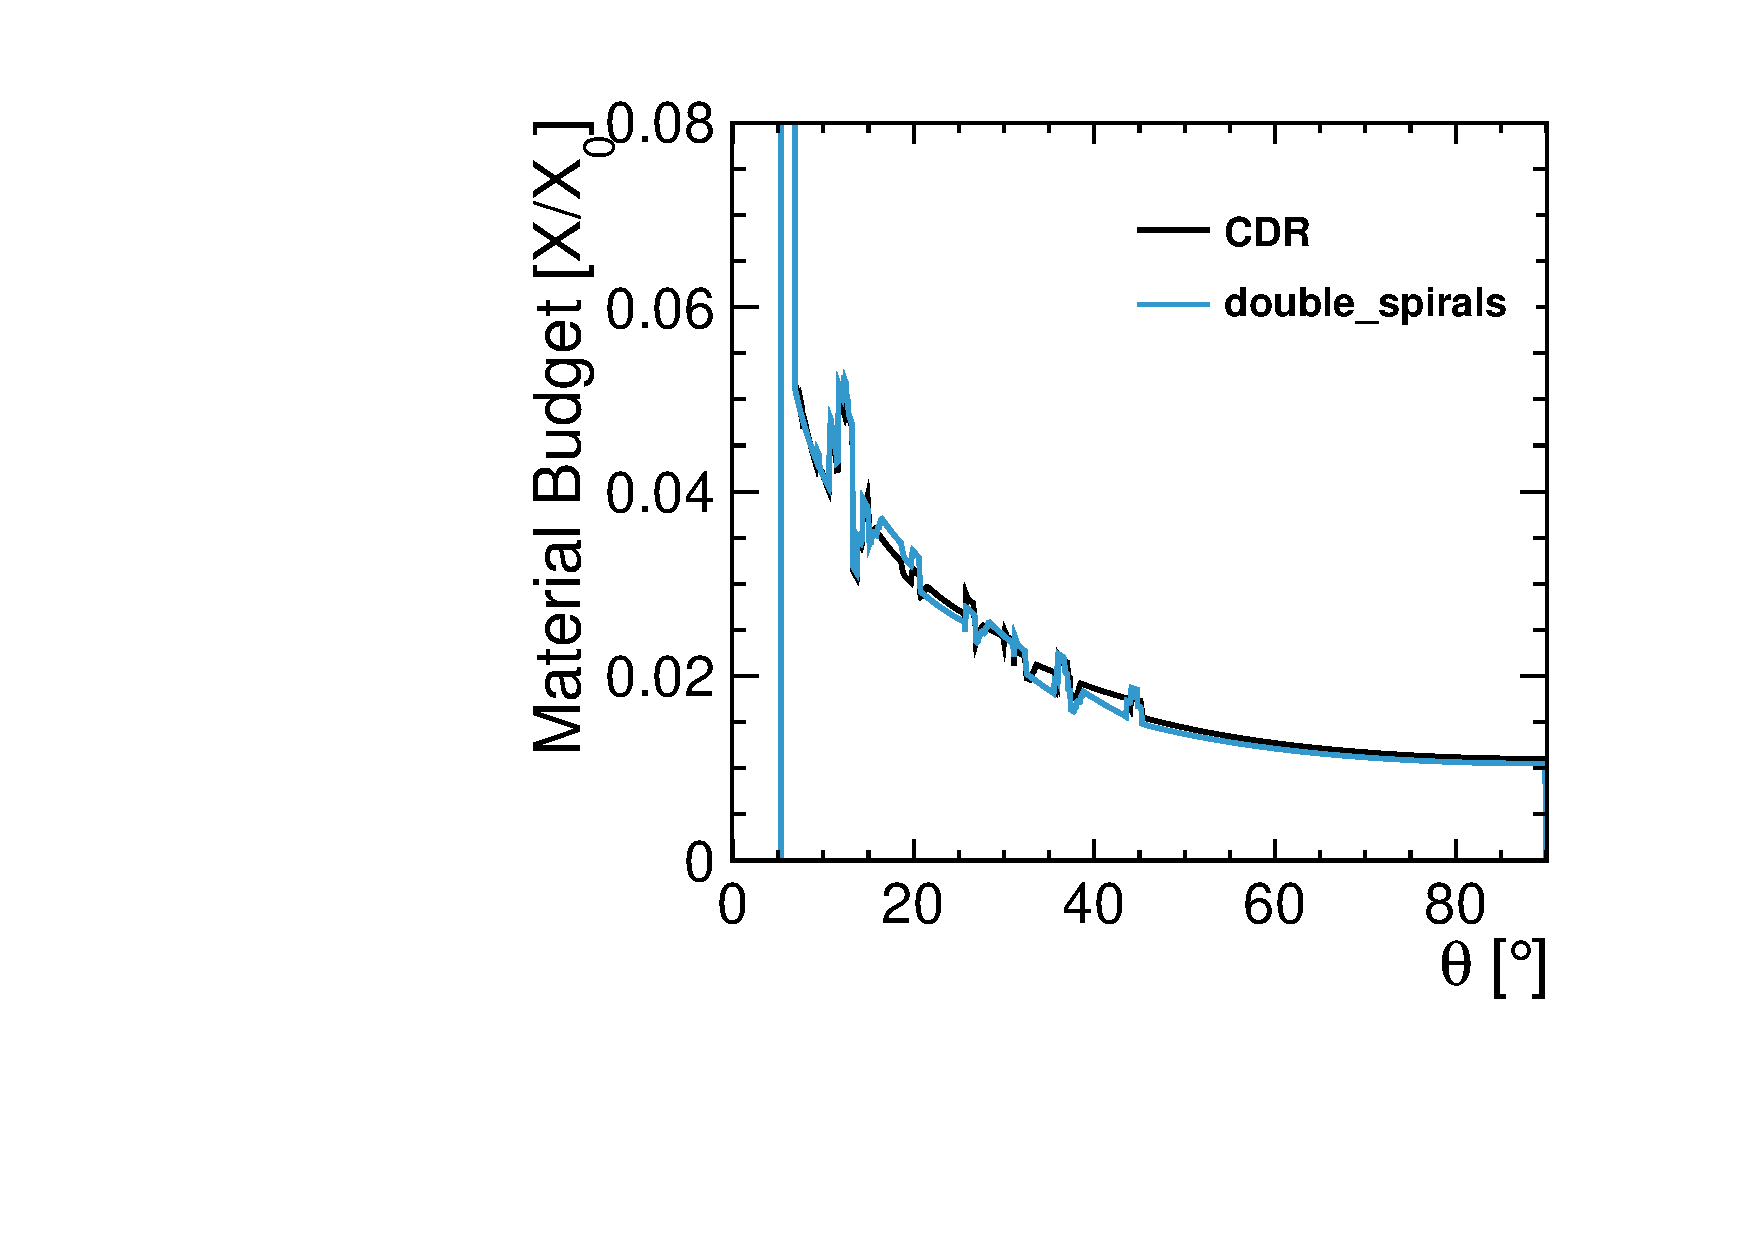
\includegraphics[scale=0.4]{Figures/Geometries/material_budget_double_spirals.pdf}
    \caption{}\label{fig:materialBudgSpiralEndcap_double}
\end{subfigure} \quad
  \begin{subfigure}[b]{0.5\textwidth}
    \centering
    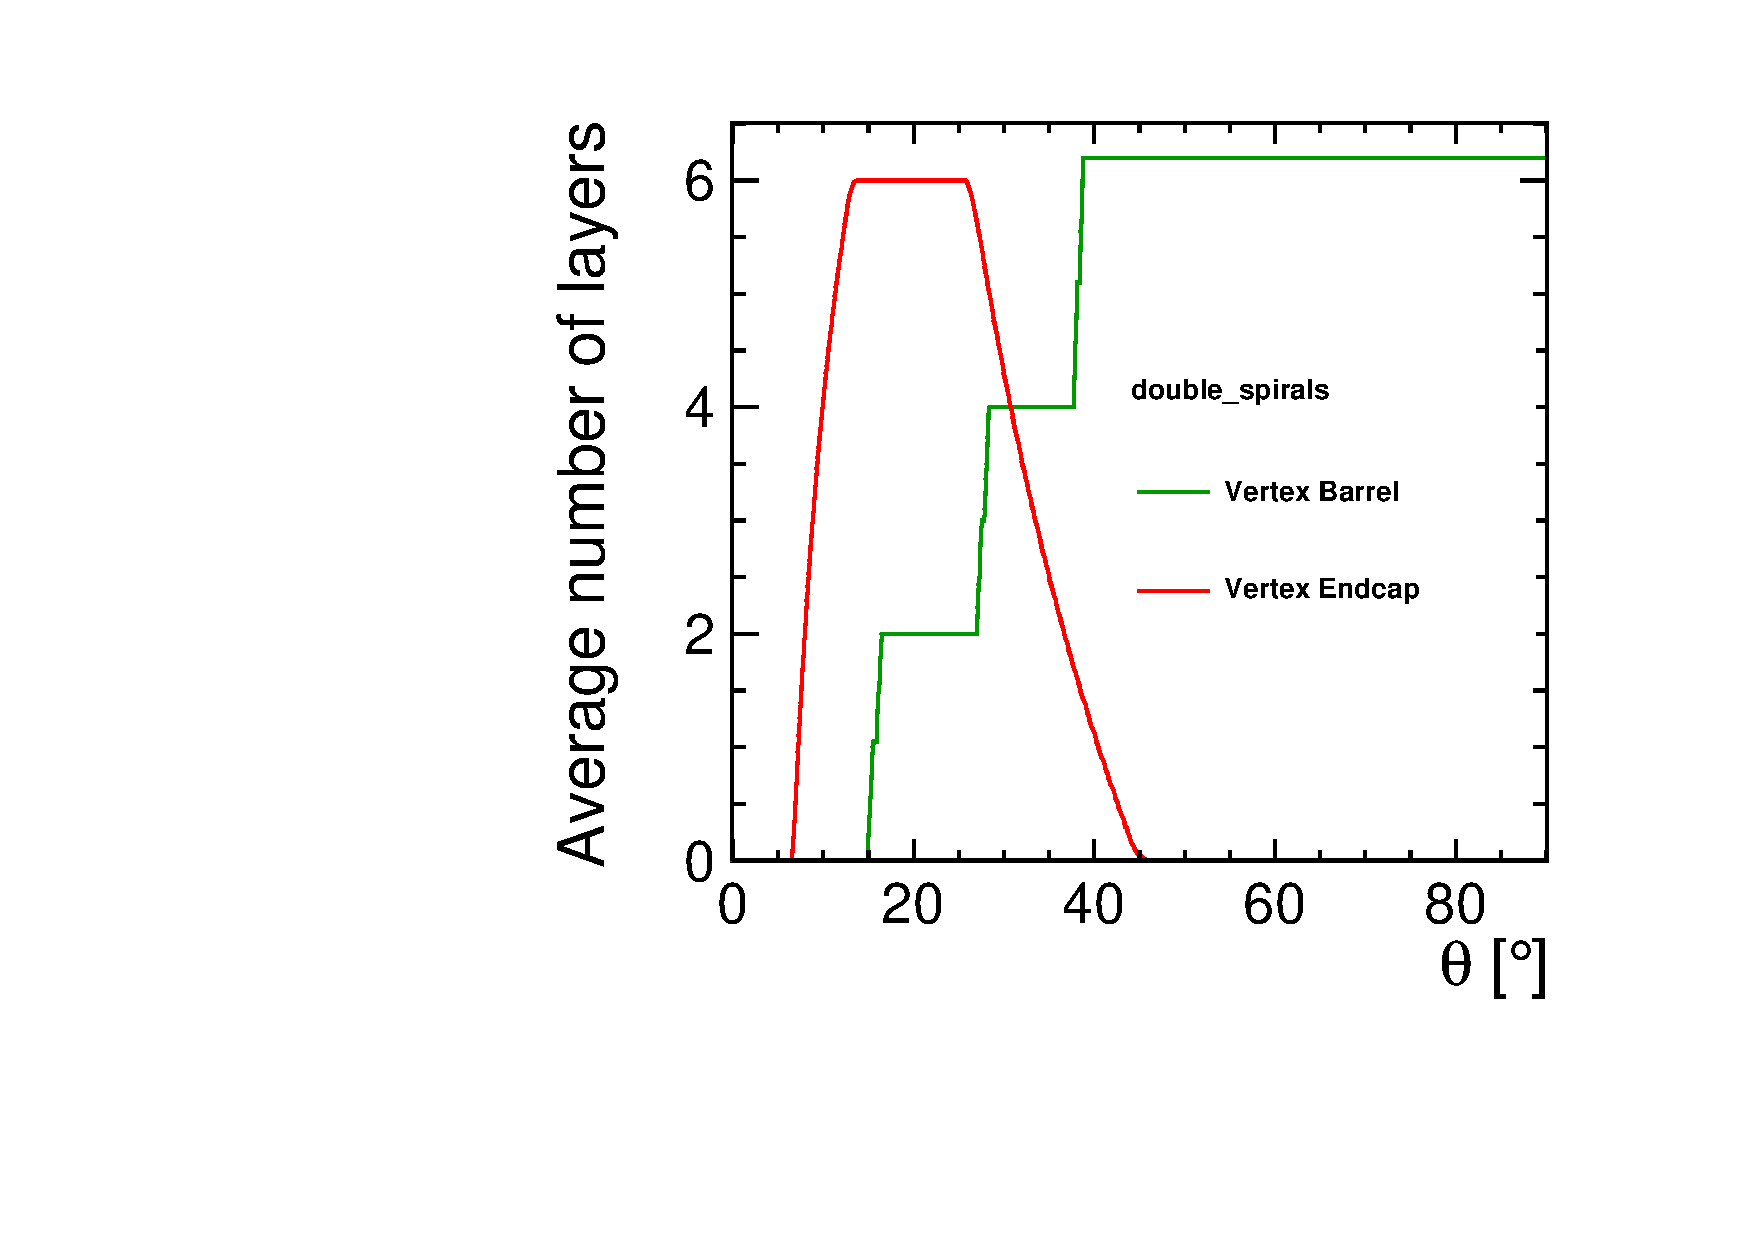
\includegraphics[scale=0.4]{Figures/Geometries/nb_layer_double.pdf}
    \caption{}\label{fig:double_nb_barrel_endcap}
  \end{subfigure}
  \caption{The material budget for the CDR and the {\it double\_spirals} vertex detectors is shown in (a). The coverage of the vertex detector for the {\it double\_spirals} geometry with respect to the polar angle $\theta$ is shown in (b). The material budget and the number of layers for each polar angle $\theta$ are averaged over the azimuthal angle $\phi$.}
\end{figure}

\newpage
As a cross-check, we have also calculated the material budget for both geometries at a polar angle of $\theta = 90^{\circ}$ using the thicknesses of all the material used. The calculated and the simulated values are compared in Table~\ref{tab:material_budg_DL_table}. We can observe that both values are quite similar, but the simulation gives higher values. This can be explained by the fact that for the simulation, the material budget is integrated over the $\phi$ angle and for some azimuthal angles the modules overlap. The calculation, on the other hand, does not consider these overlaps. 

\begin{table}[H]
  \caption{Calculated and simulated values of the material budget for the CDR and the \textit{double\_spirals} vertex barrel at $\theta = 90^{\circ}$ in units of $X_{0}$.}
  \begin{center}
    \begin{tabular}{ c  c  c } \hline
      & CDR & \textit{double\_spirals} \\  \hline \hline
      Calculation & $1.07\%$ & $1.00\%$ \\ \hline
      Simulation & $1.10\%$ & $1.05\%$ \\ \hline
    \end{tabular}
  \end{center}
  \label{tab:material_budg_DL_table}
\end{table}


Figure~\ref{fig:vertex_nb_layer} summarizes the coverage of the whole vertex detector (the vertex barrel and endcaps) for the above-mentioned geometries with respect to the polar angle $\theta$ (averaged over $\phi$). Overall, the \begin{it}double\_spirals\end{it} geometry has more sensitive layers in the barrel and the endcaps with similar material budget as the CDR and the \begin{it}spirals\end{it} geometries. 


\begin{figure}[H]
  \centering
  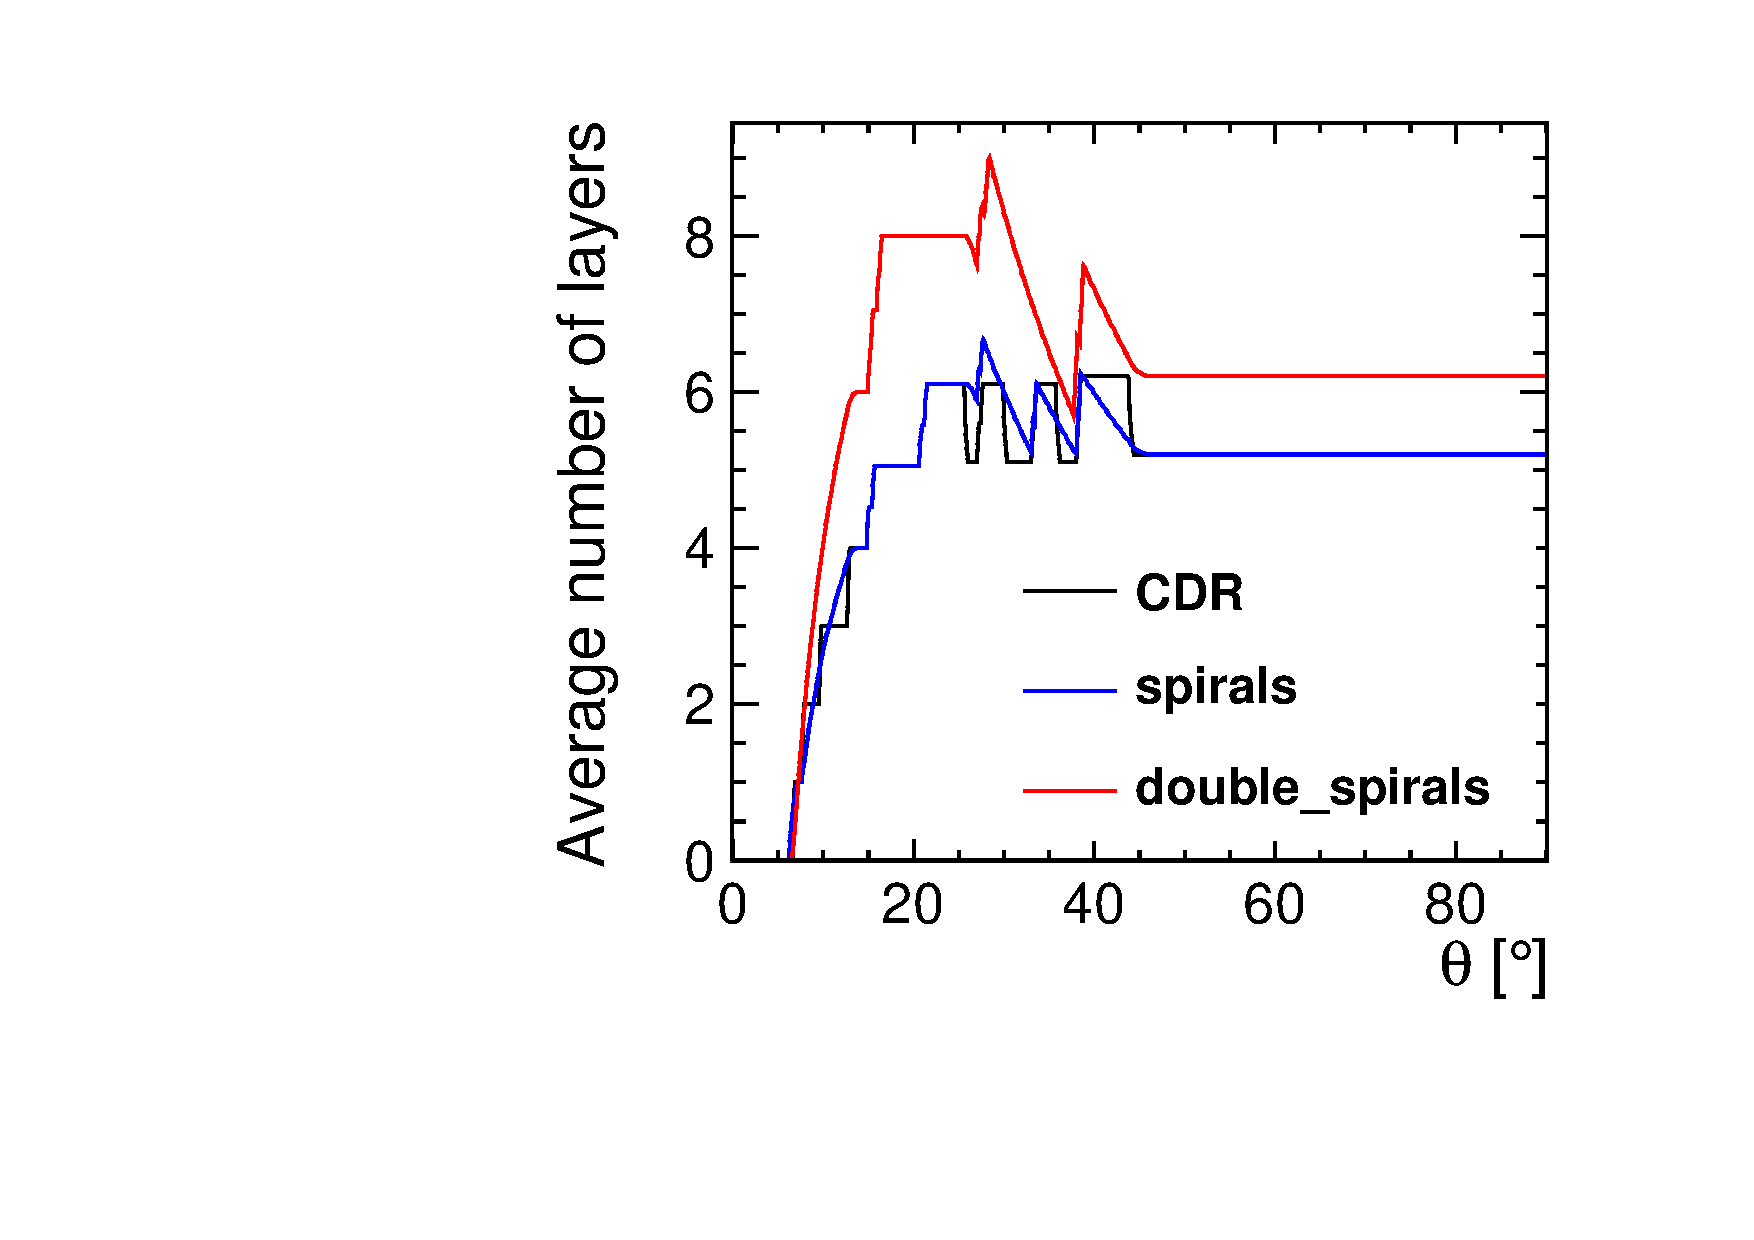
\includegraphics[scale=0.4]{Figures/Geometries/avg_nb_layers_allGeoms.pdf}
  \caption{The coverage of the vertex detector for 3 different geometries with respect to the polar angle $\theta$. The number of sensitive layers are averaged over the azimuthal angle $\phi$.}
  \label{fig:vertex_nb_layer}
\end{figure}

Figure~\ref{fig:nbLayers_theta_phi} shows the number of layers as function of the polar angle $\theta$ and the azimuthal angle $\phi$ for the \begin{it}spirals\end{it} and the \begin{it}double\_spirals\end{it} geometries in the endcap regions. For polar angles around $\theta=40^{\circ}$, the number of layers becomes very dependent on the azimuthal angle $\phi$. In this region, there is a transition between the endcaps and the barrel sections. Using a spiral arrangement of the sensors in the vertex endcaps introduces a $\phi$ asymmetry in the coverage, see Figures~\ref{fig:singleSpiralGeom} and \ref{fig:doubleSpiralGeom}.
For some discrete $\phi$ angles, the number of layers is twice the one
at neighbouring $\phi$ angles (Figure~\ref{fig:nbLayers_theta_phi}). This can be explained by the fact that for a given  $\theta$, neighboring modules have a small overlap in $\phi$.

\begin{figure}[H]
        \begin{subfigure}[b]{0.5\textwidth}
          \centering
          %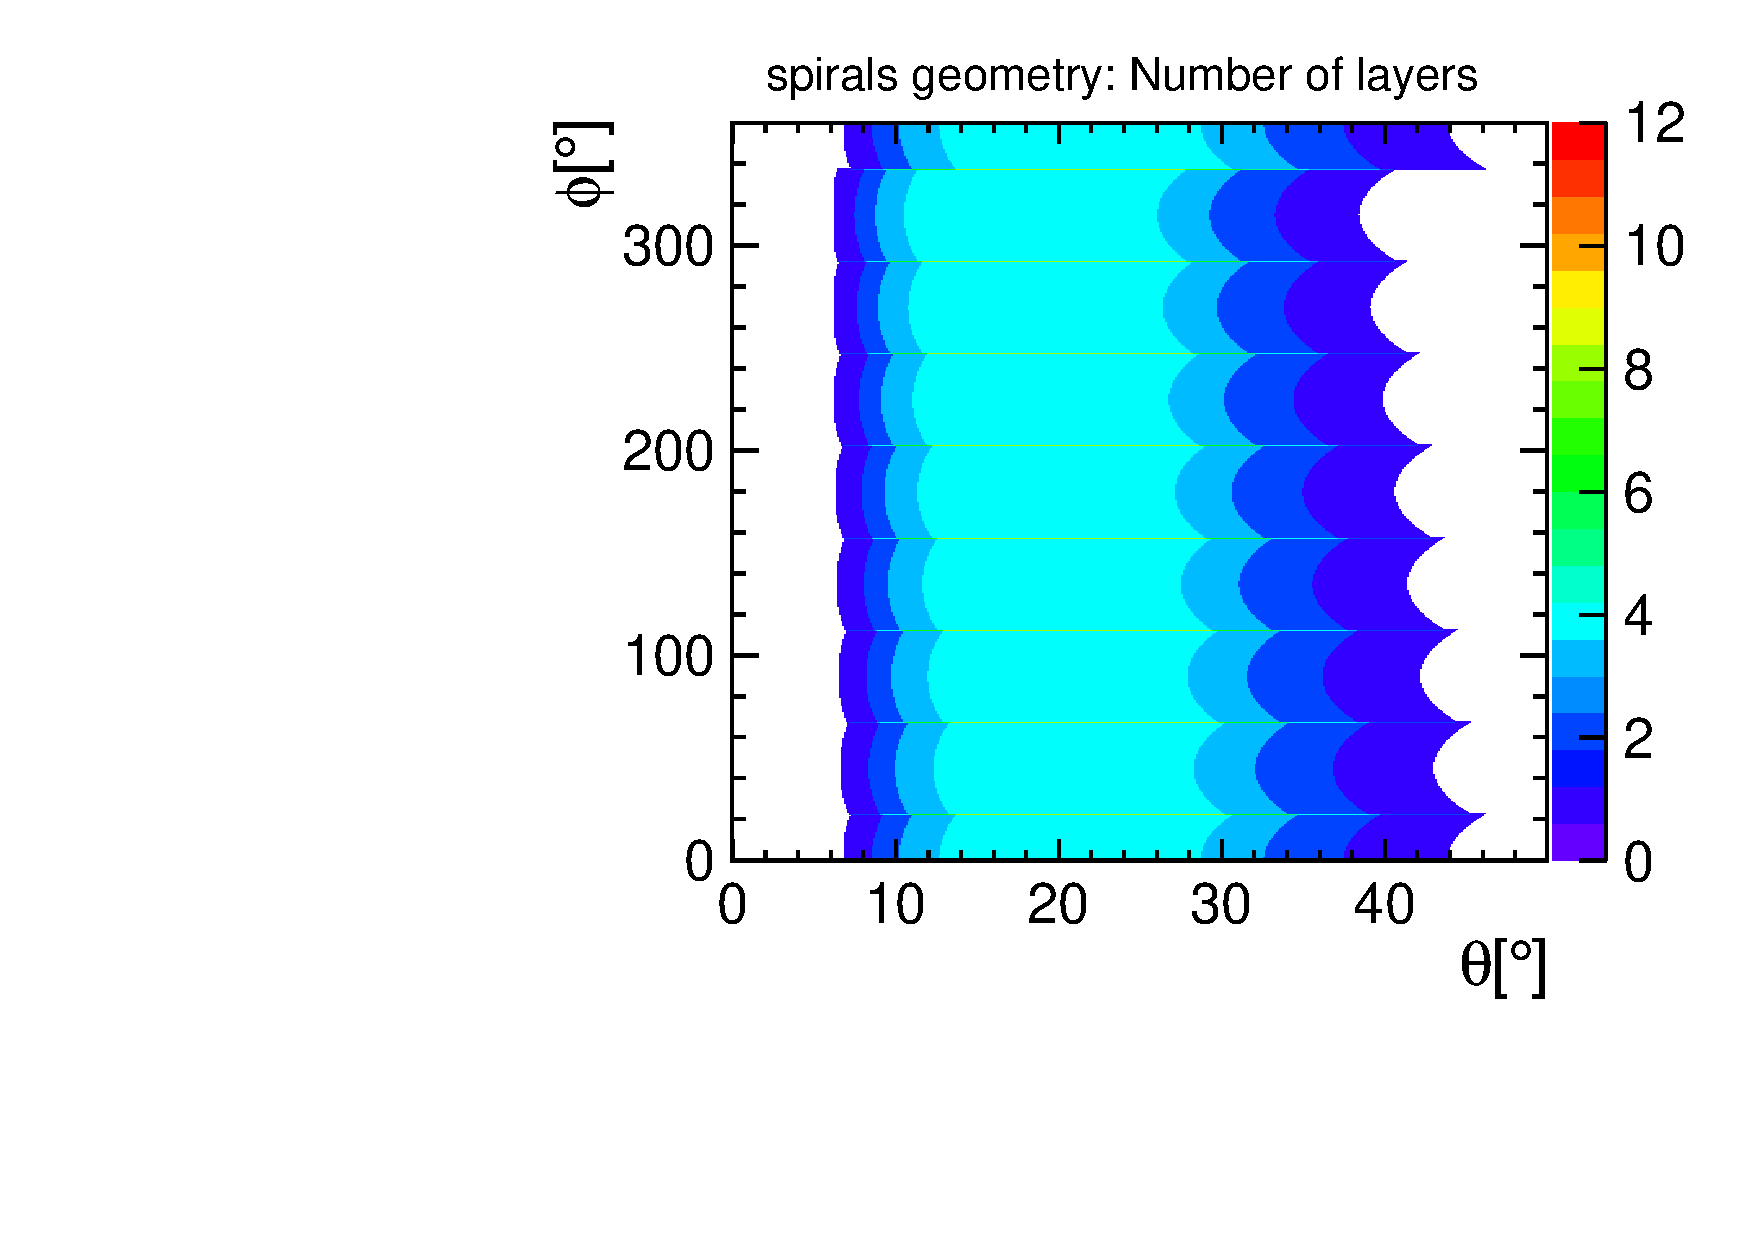
\includegraphics[width=\textwidth]{Figures/Geometries/spirals_theta_phi.pdf}
          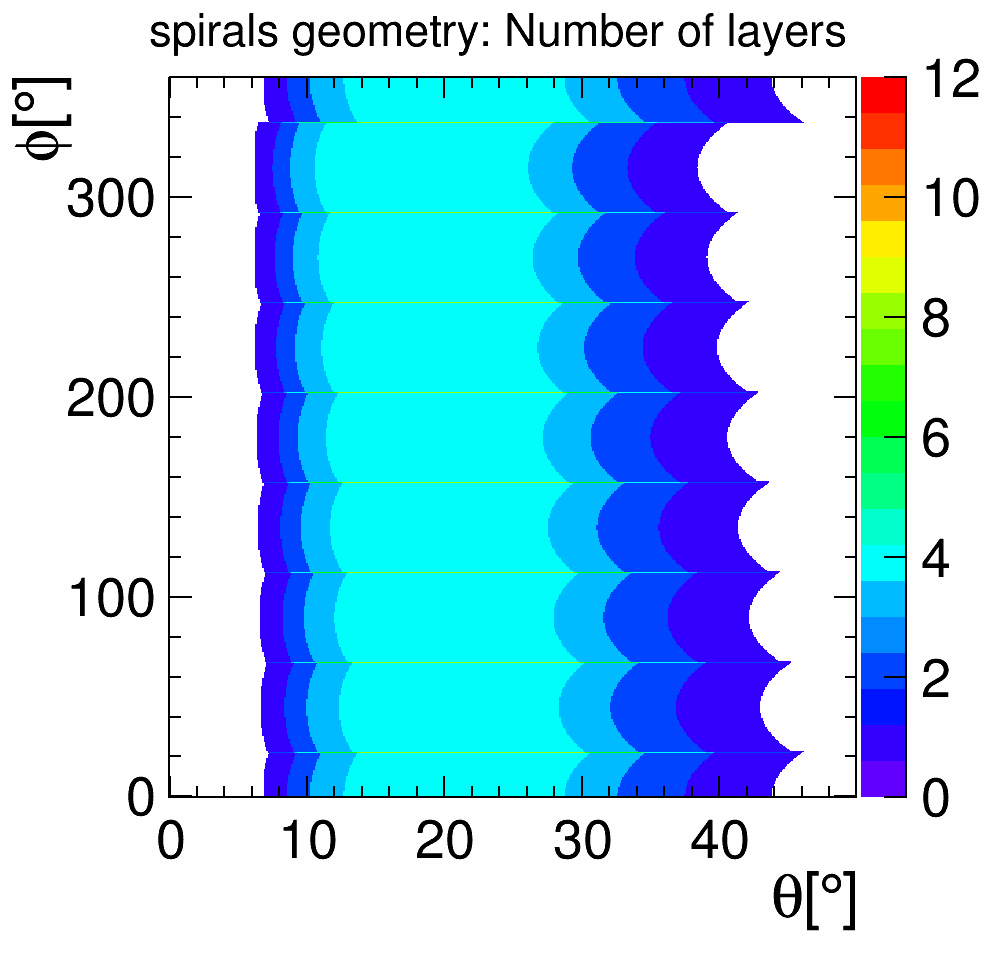
\includegraphics[width=\textwidth]{Figures/Geometries/spirals.png}
          \caption{}
          \label{}
        \end{subfigure}%
        ~ 
        \begin{subfigure}[b]{0.5\textwidth}
          \centering
          %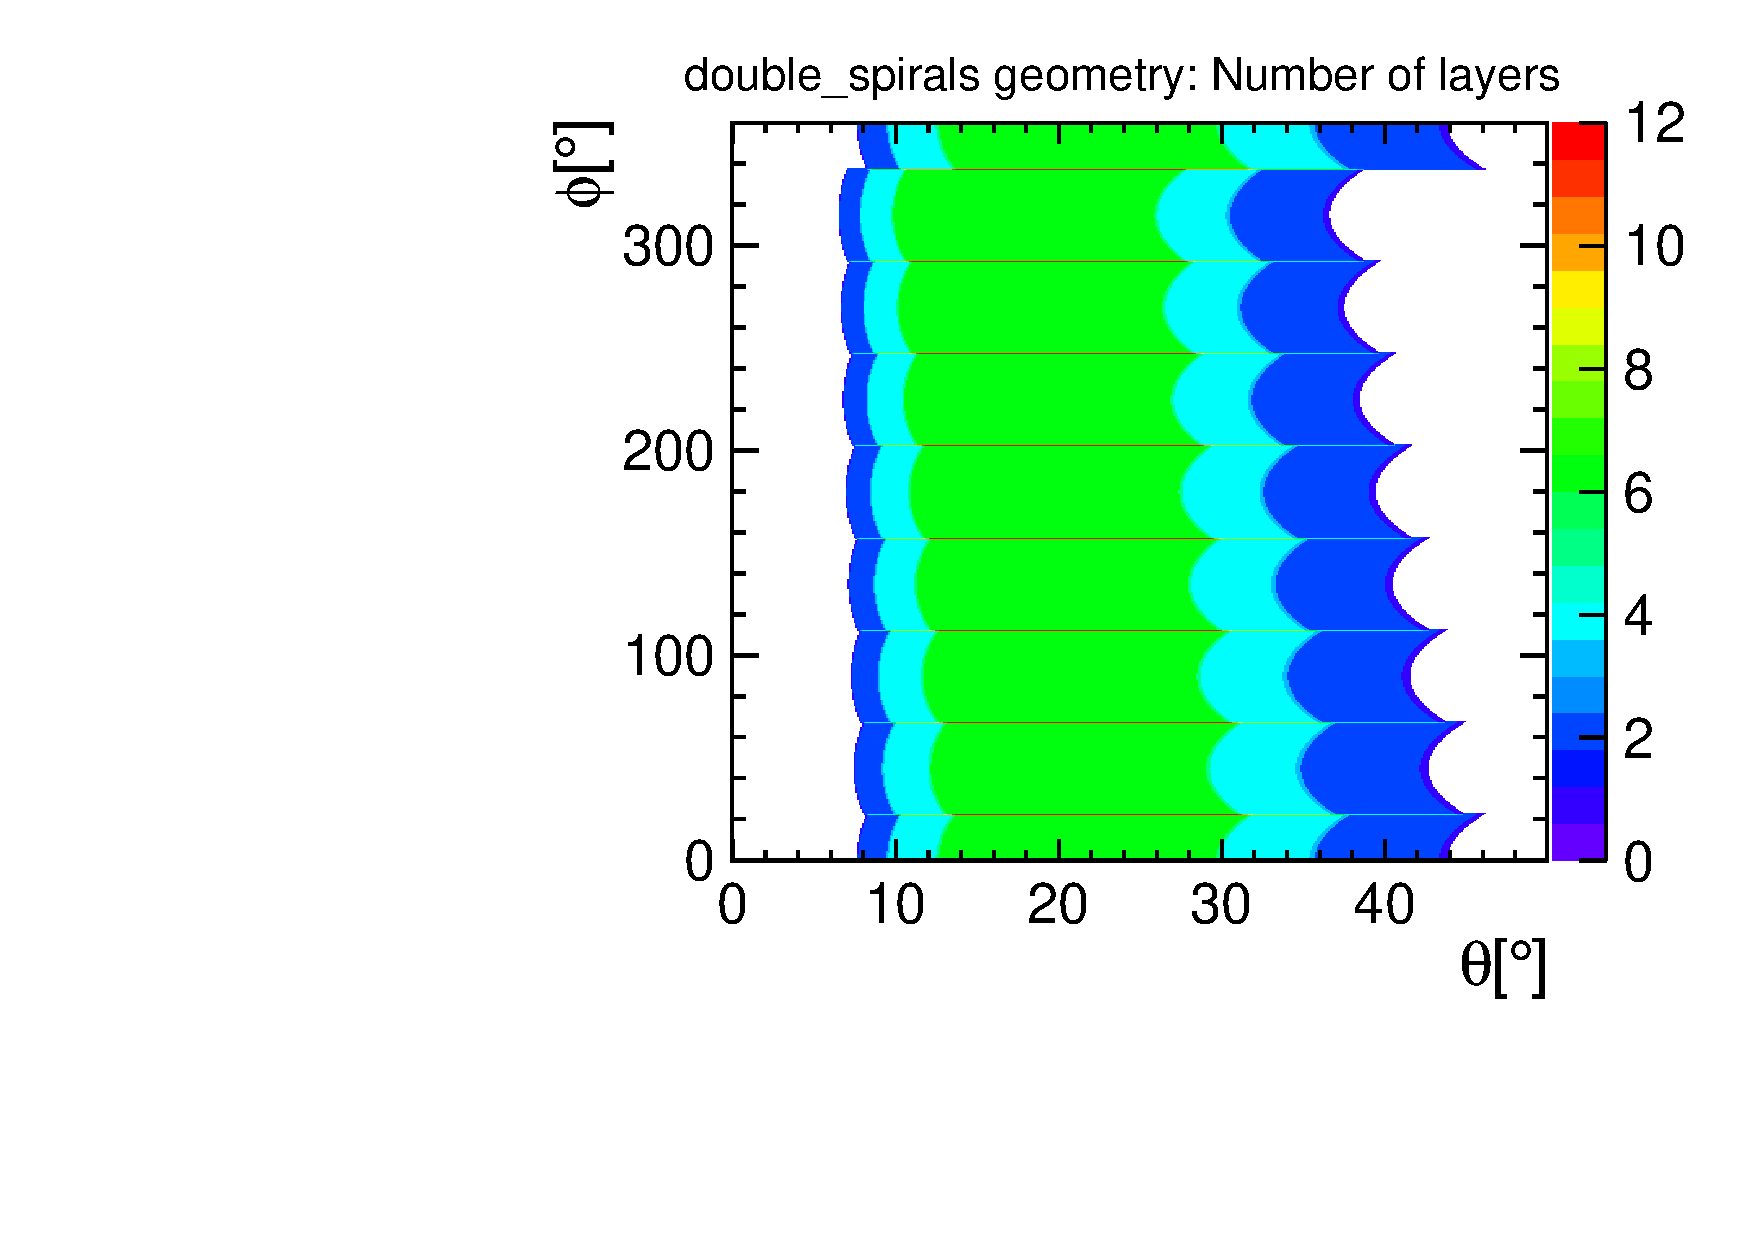
\includegraphics[width=\textwidth]{Figures/Geometries/double_spirals_theta_phi.pdf}
          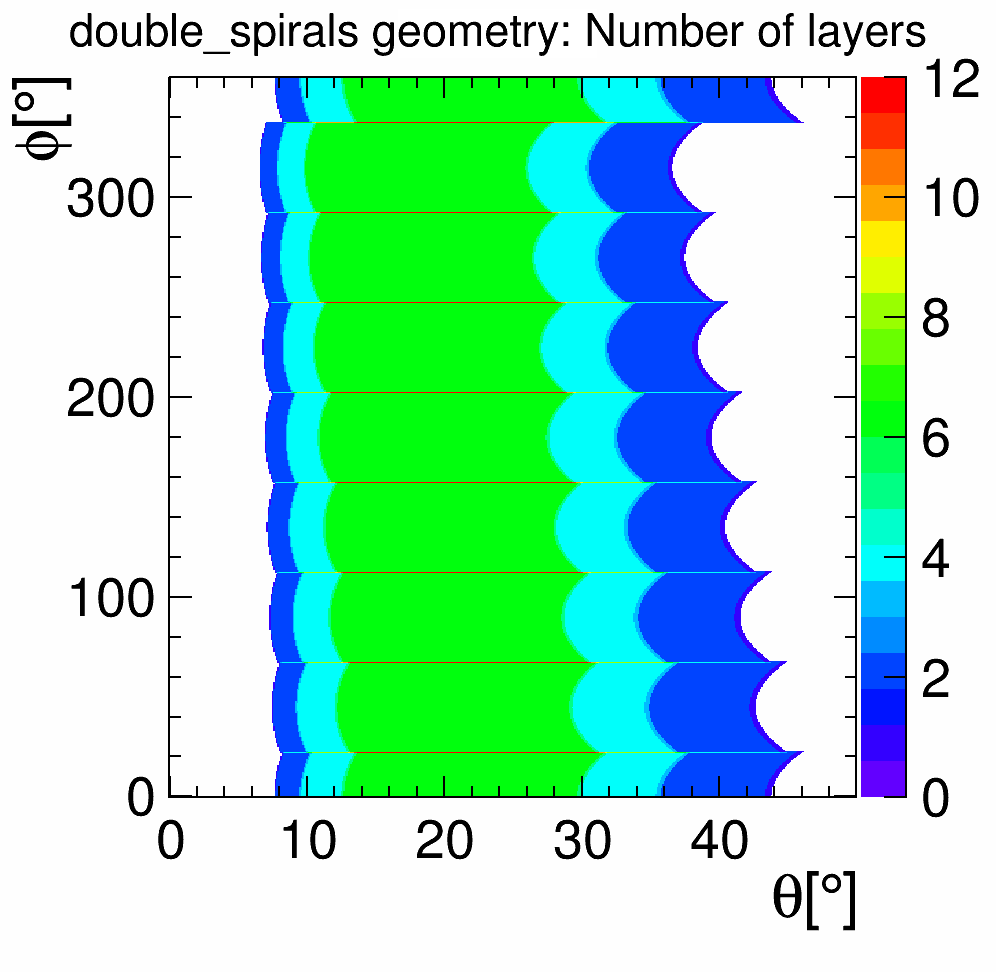
\includegraphics[width=\textwidth]{Figures/Geometries/double_spirals.png}
          \caption{}
          \label{}
        \end{subfigure}
        \caption{Number of layers as a function of the polar angle
          $\theta$ and of the azimuthal angle $\phi$ for the {\it
            spirals} and the {\it double\_spirals} geometries in the endcap regions. }\label{fig:nbLayers_theta_phi}
\end{figure}
%----------------------------------------------------------------------
\subsection{The \emph{double\_spirals\_v2} geometry}\label{sec:CLIC_SiD_double_spirals_heavy}

In engineering studies, a double-layered module is estimated to have a material budget of $0.4\%X_{0}$. This value takes into account two silicon sensors with a thickness of \SI{50}{\micro\meter}, the ASIC of \SI{50}{\micro\meter}, the carbon fiber for the mechanical support, the electronics used for the power pulsing and the cables~\cite{Blanchot:1635206}. \\
The \begin{it}double\_spirals\_v2\end{it} geometry has the same layout
as \begin{it}double\_spirals\end{it}
(cf. Section~\ref{sec:CLIC_SiD_double_spirals}), but with a material
budget of $0.4\%X_{0}$ per double layer. In the simulation, this was
achieved by modules of silicon followed by \SI{13.5}{\micro\meter} of
copper. The material budget for the \textit{double\_spirals\_v2} geometry is for example 1.6 times higher at $\theta=90^{\circ}$ than that of the CDR geometry as shown in Figure~\ref{fig:material_budget_heavy_double_spirals}.

\begin{figure}[H]
  \centering
    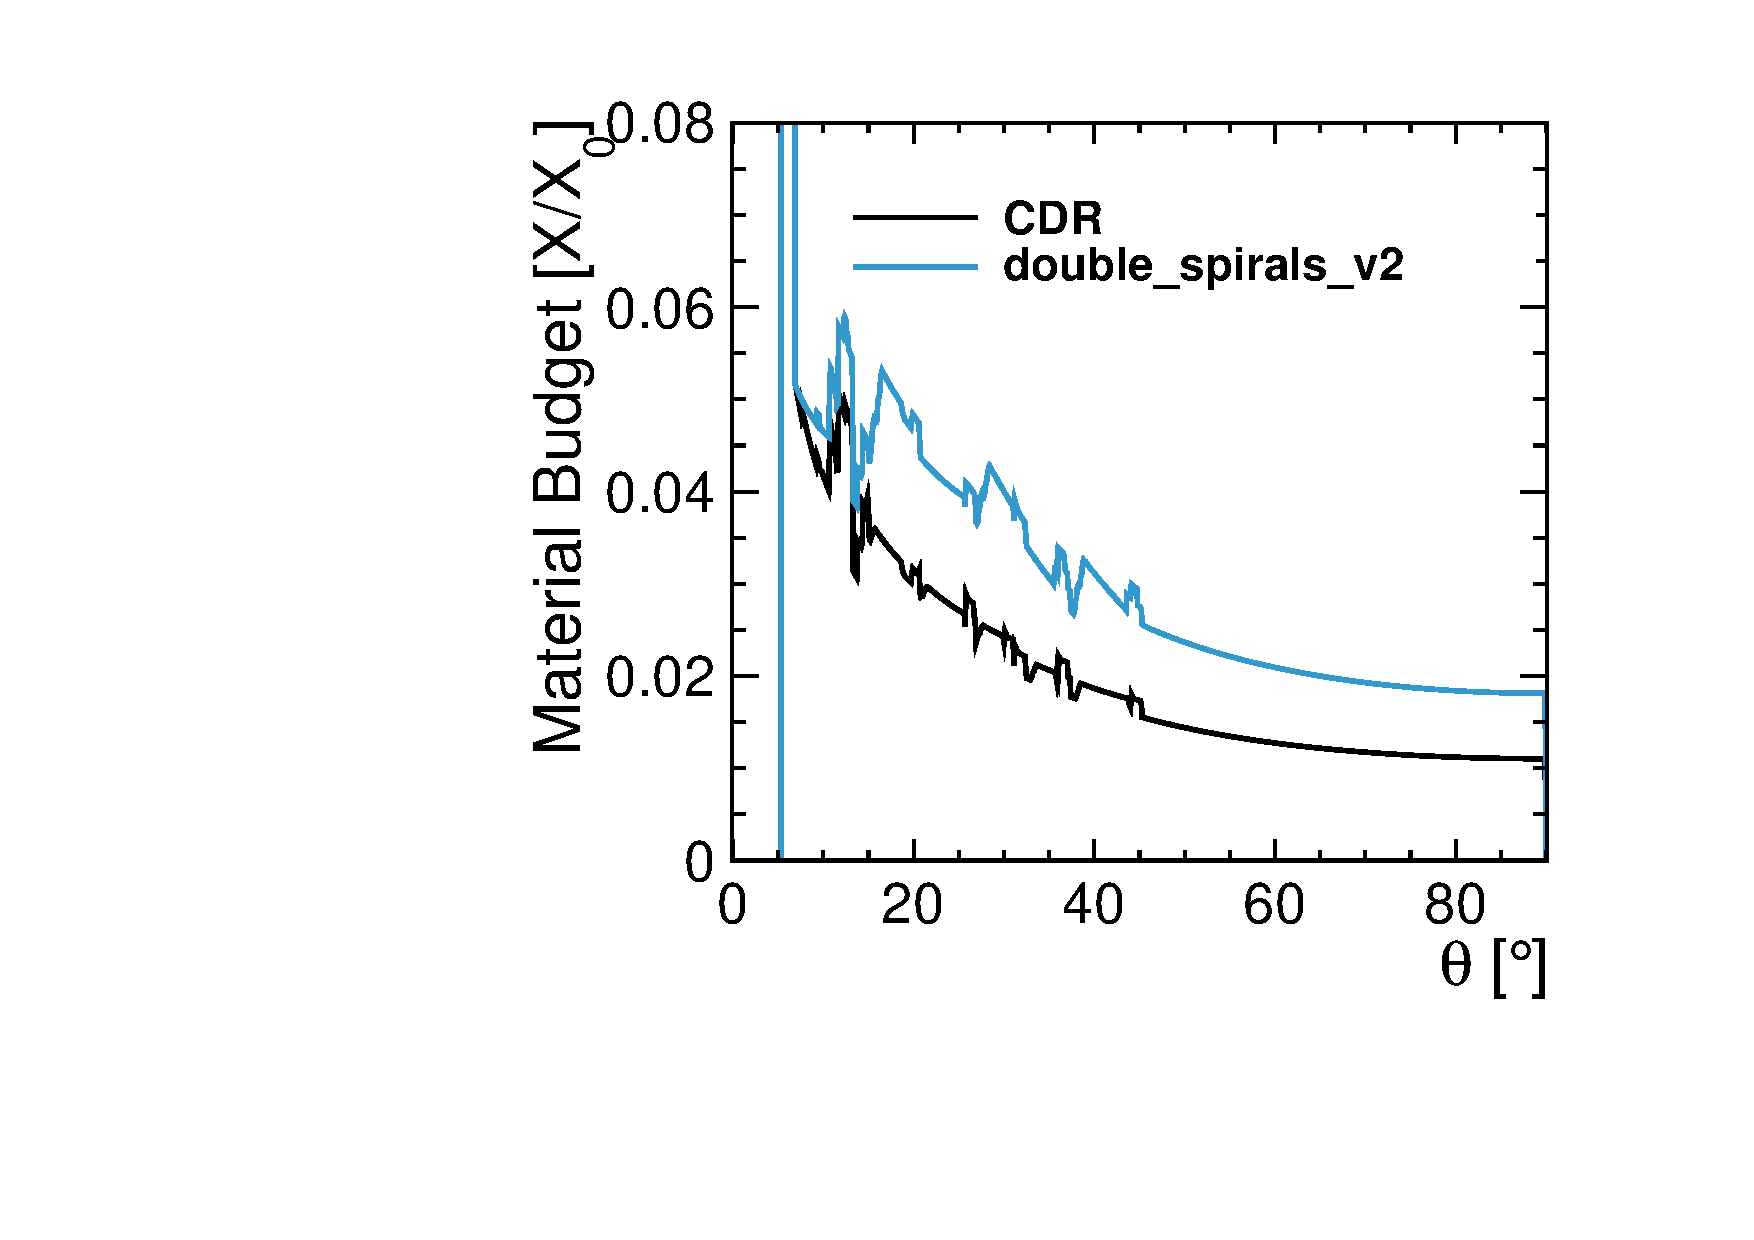
\includegraphics[scale=0.4]{Figures/Geometries/material_budget_heavy_double_spirals.pdf}
    \caption{The simulated material budget for the CDR and {\it double\_spirals\_v2} geometries. For each polar angle $\theta$, the material budget is averaged over the azimuthal angle $\phi$.}
    \label{fig:material_budget_heavy_double_spirals}
\end{figure}

%
\section{Tracking Performance}\label{sec:trackingPerformance}

The momentum resolution $\sigma(\Delta p/{p^{2}}_{True})$ as well as the
transverse $\sigma(\Delta d_{0})$ and longitudinal $\sigma(\Delta z_{0})$ impact parameter resolutions are compared for the different implemented geometries using single muons with momenta of 1, 10 and 100~GeV for different polar and azimuthal angles. The resolutions are obtained from a Gaussian fit using at least 10000 simulated events and reconstructed tracks.
The statistical errors on the impact parameter resolutions are also given in the plots and they are negligible.

\subsection{The \emph{spirals} geometry}

%% The momentum and the transverse and longitudinal impact parameter resolutions are computed for the CDR and the spirals geometries using single muons with a polar angle of $\theta = 20^\circ$ and momenta of 1, 10 and 100~GeV as shown in Figure \ref{fig:spiralRes}. The points are obtained from a Gaussian fit using at least 10000 simulated events and reconstructed tracks. \\
To study the impact of the \begin{it}spirals\end{it} geometry on the tracking performance, single muons are used with a polar angle of $\theta=20^{\circ}$ and azimuthal angles of $\phi=180^{\circ}$ or $\phi=225^{\circ}$ which hit the first and the last modules of the first endcap layer, respectively. Figure~\ref{fig:spiralRes} compares the $p$, $d_{0}$ and $z_{0}$ resolutions for the CDR and the \begin{it}spirals\end{it} geometries. \\
%% In Figure \ref{fig:spiralRes} we also want to see how much the resolution changes from one module of the endcap to the other as the modules for each endcap layer are situated in different z positions. For this purpose, we have chosen two different azimuthal angles $\phi=180^\circ$ and $\phi=135^\circ$ which respectively correspond to the first module and the last module of the first endcap layer as shown in Figure \ref{fig:spiralEndcapsPhis}.
The momentum resolutions are very similar in all cases as the measurement of the momentum is dominated by the main tracker. The spiral arrangement affects the $d_0$ and $z_0$ resolutions in the forward direction. This can be explained by the fact that the measurement of these two parameters depends on the distance of the vertex layers to the interaction point. \\
These results are in a reasonable agreement with the results presented in the CDR.

\begin{figure}[H]
  %\hspace{-2cm}
        %\centering
        \begin{subfigure}[b]{0.4\textwidth}
          \centering
          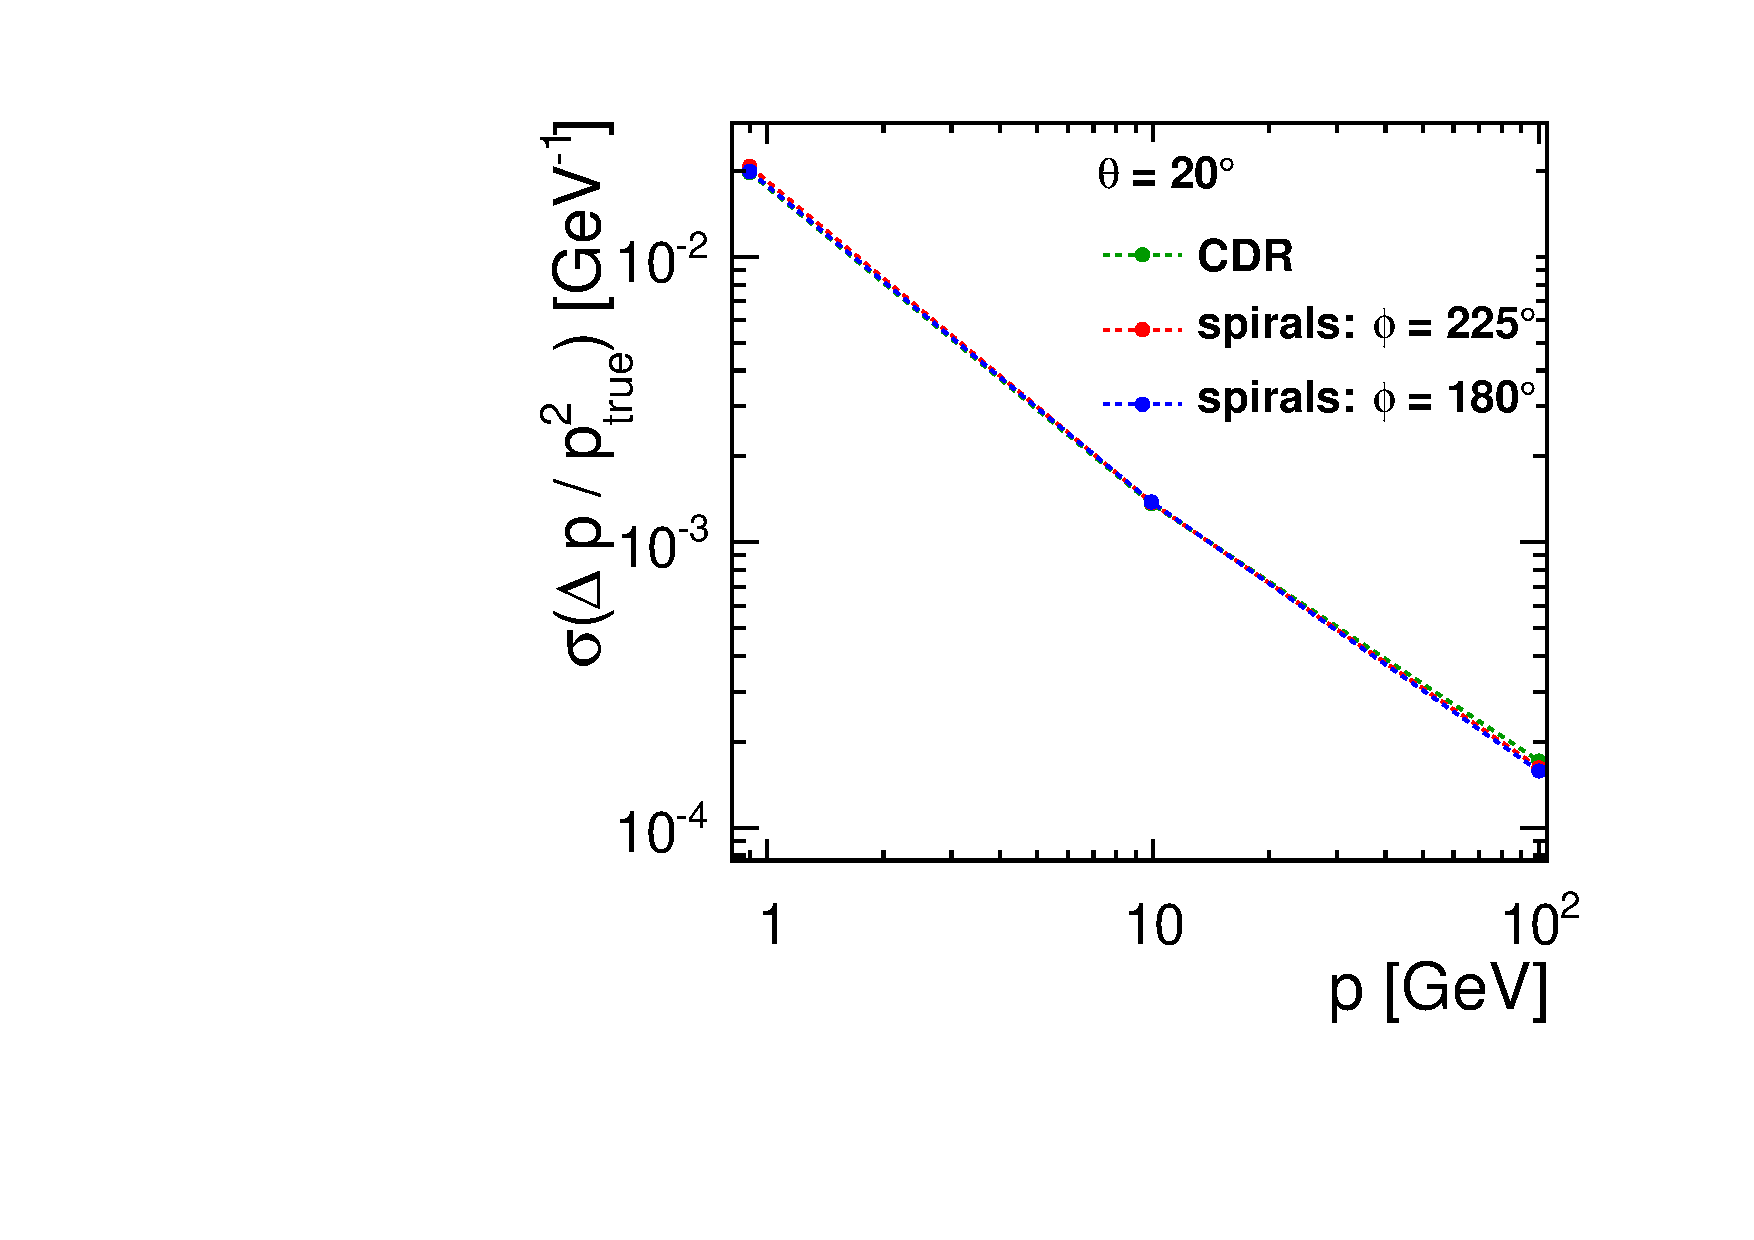
\includegraphics[width=\textwidth]{Figures/Geometries/pT_resolution_spirals.pdf}
          \caption{Momentum resolution}
          \label{}
        \end{subfigure}%
        ~ 
        \begin{subfigure}[b]{0.4\textwidth}
          \centering
          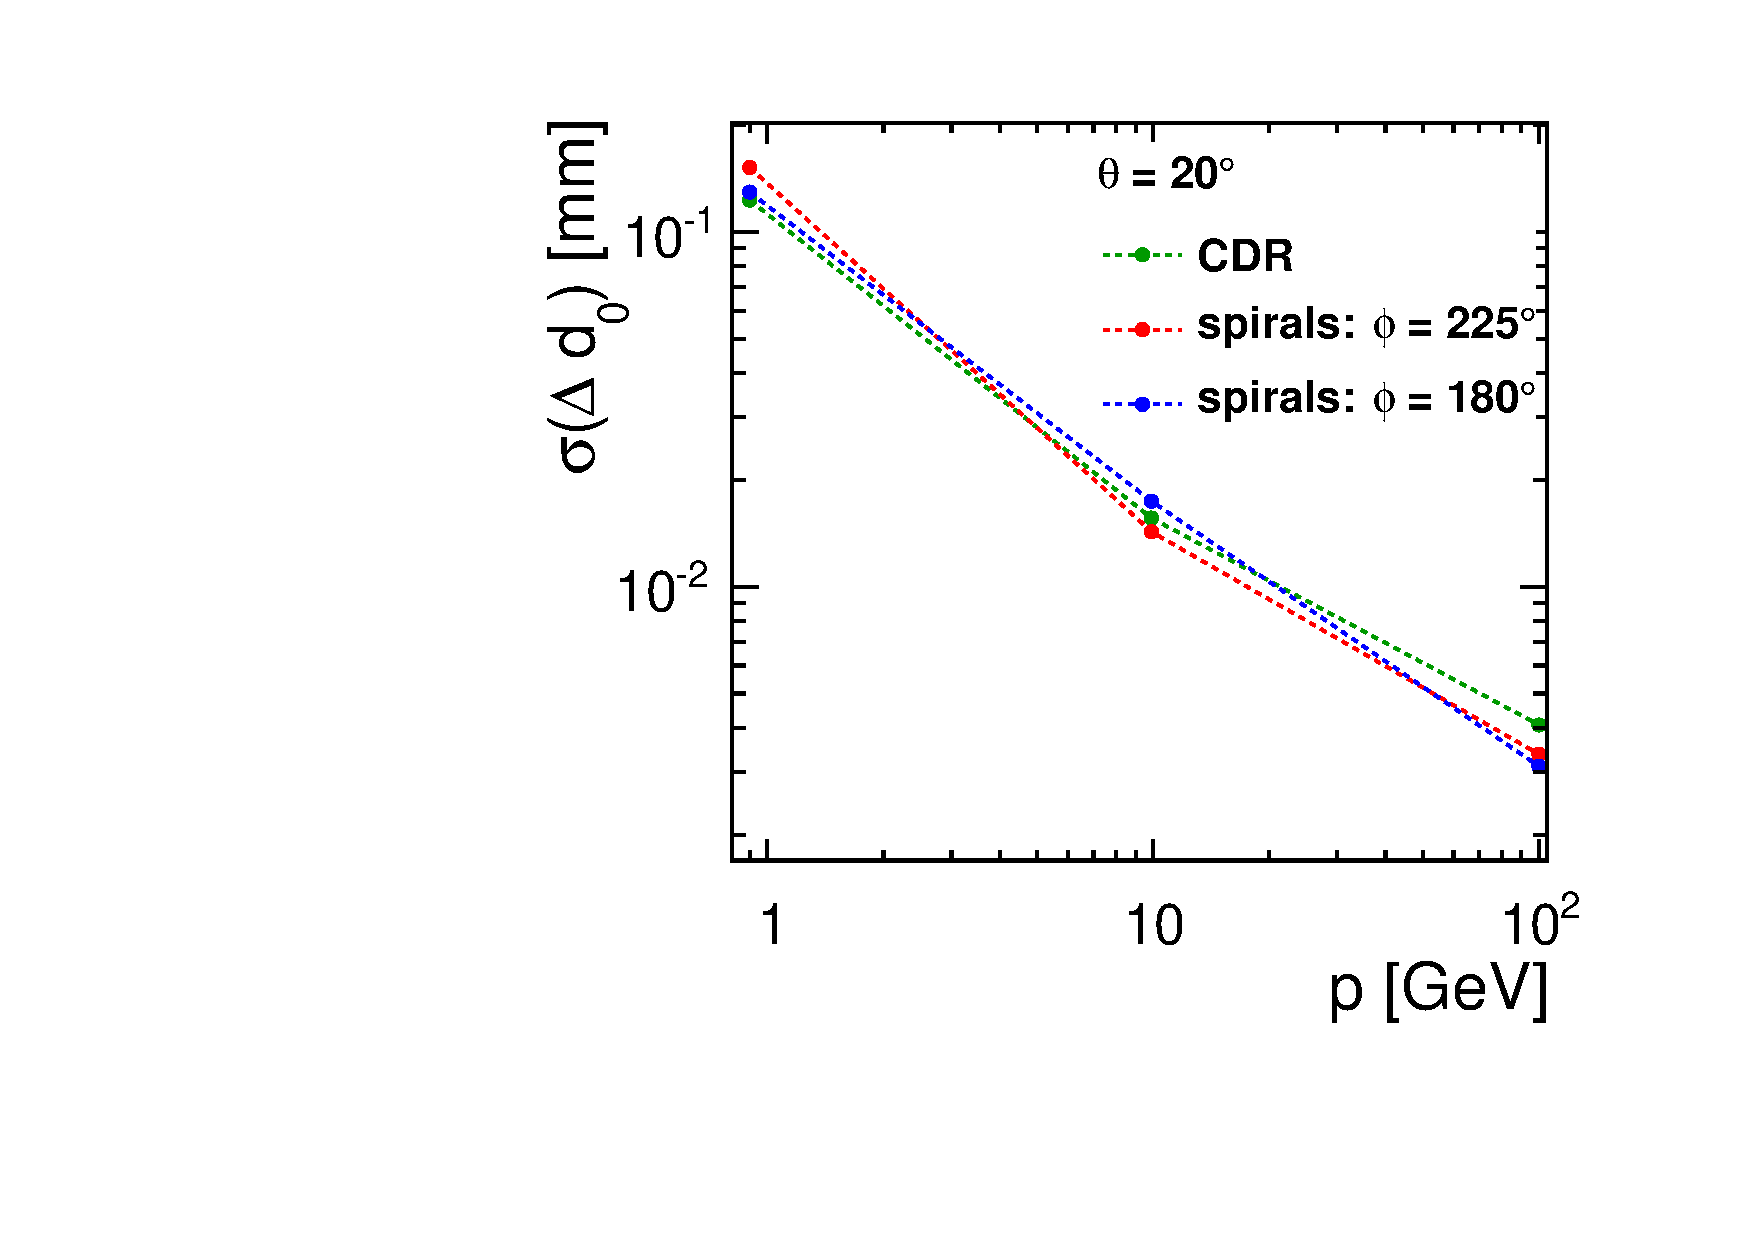
\includegraphics[width=\textwidth]{Figures/Geometries/d0_resolution_spirals.pdf}
          \caption{Transverse impact-parameter resolution}
          \label{}
        \end{subfigure}
        ~
        \begin{subfigure}[b]{\textwidth}
          \centering
          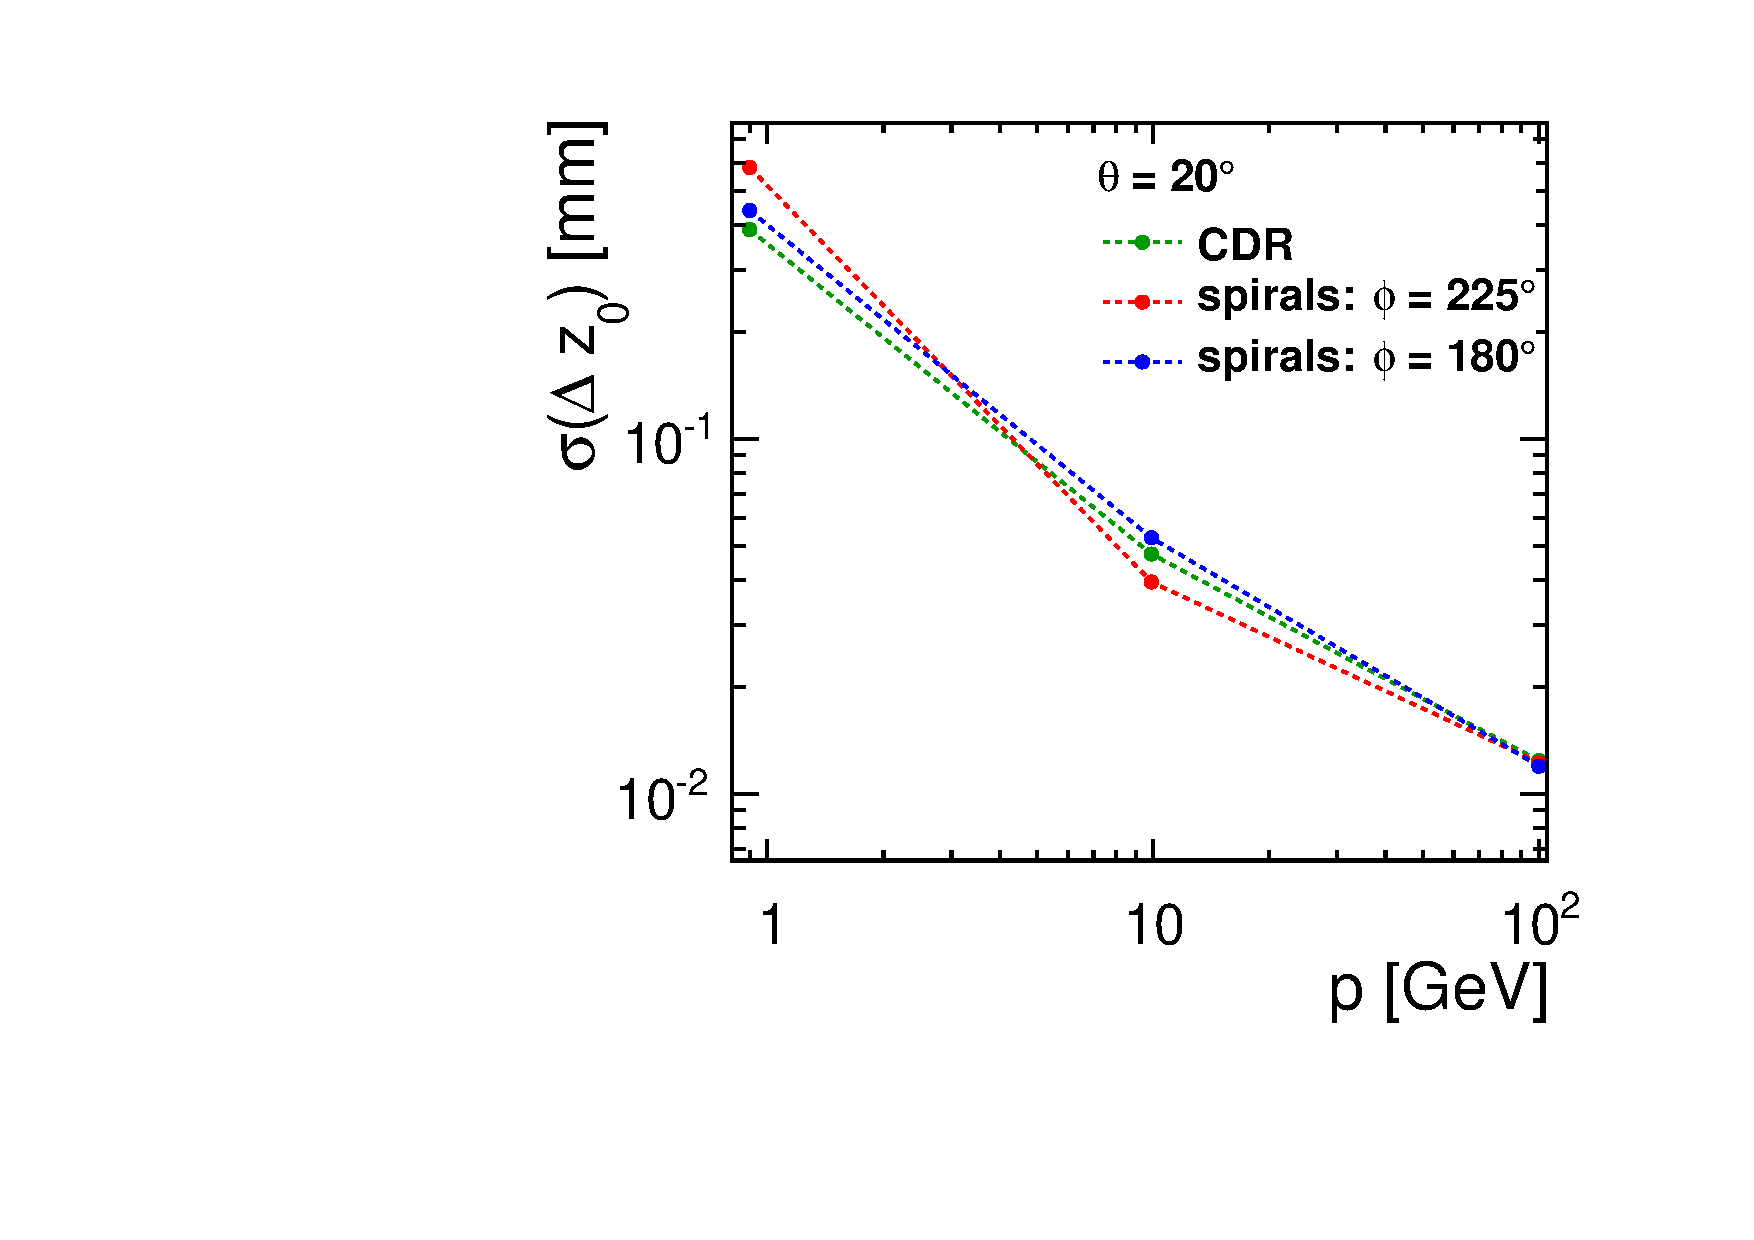
\includegraphics[width=0.4\textwidth]{Figures/Geometries/z0_resolution_spirals.pdf}
          \caption{Longitudinal impact-parameter resolution}
          \label{}
        \end{subfigure}
        \caption{(a) Momentum, (b) transverse impact-parameter and
          (c) longitudinal impact-parameter resolutions for the CDR and
          the {\it spirals} geometries for single muons at $\theta = 20^\circ$.}\label{fig:spiralRes}
\end{figure}


\subsection{The \emph{double\_spirals} geometry}
The effect of the \begin{it}double\_spirals\end{it} geometry on the tracking performance in the barrel region is studied for single muons with a polar angle of $\theta=90^\circ$ in Figure~\ref{fig:doubleLayerRes}.


\begin{figure}[H]
        \centering
        \begin{subfigure}[b]{0.4\textwidth}
          \centering
          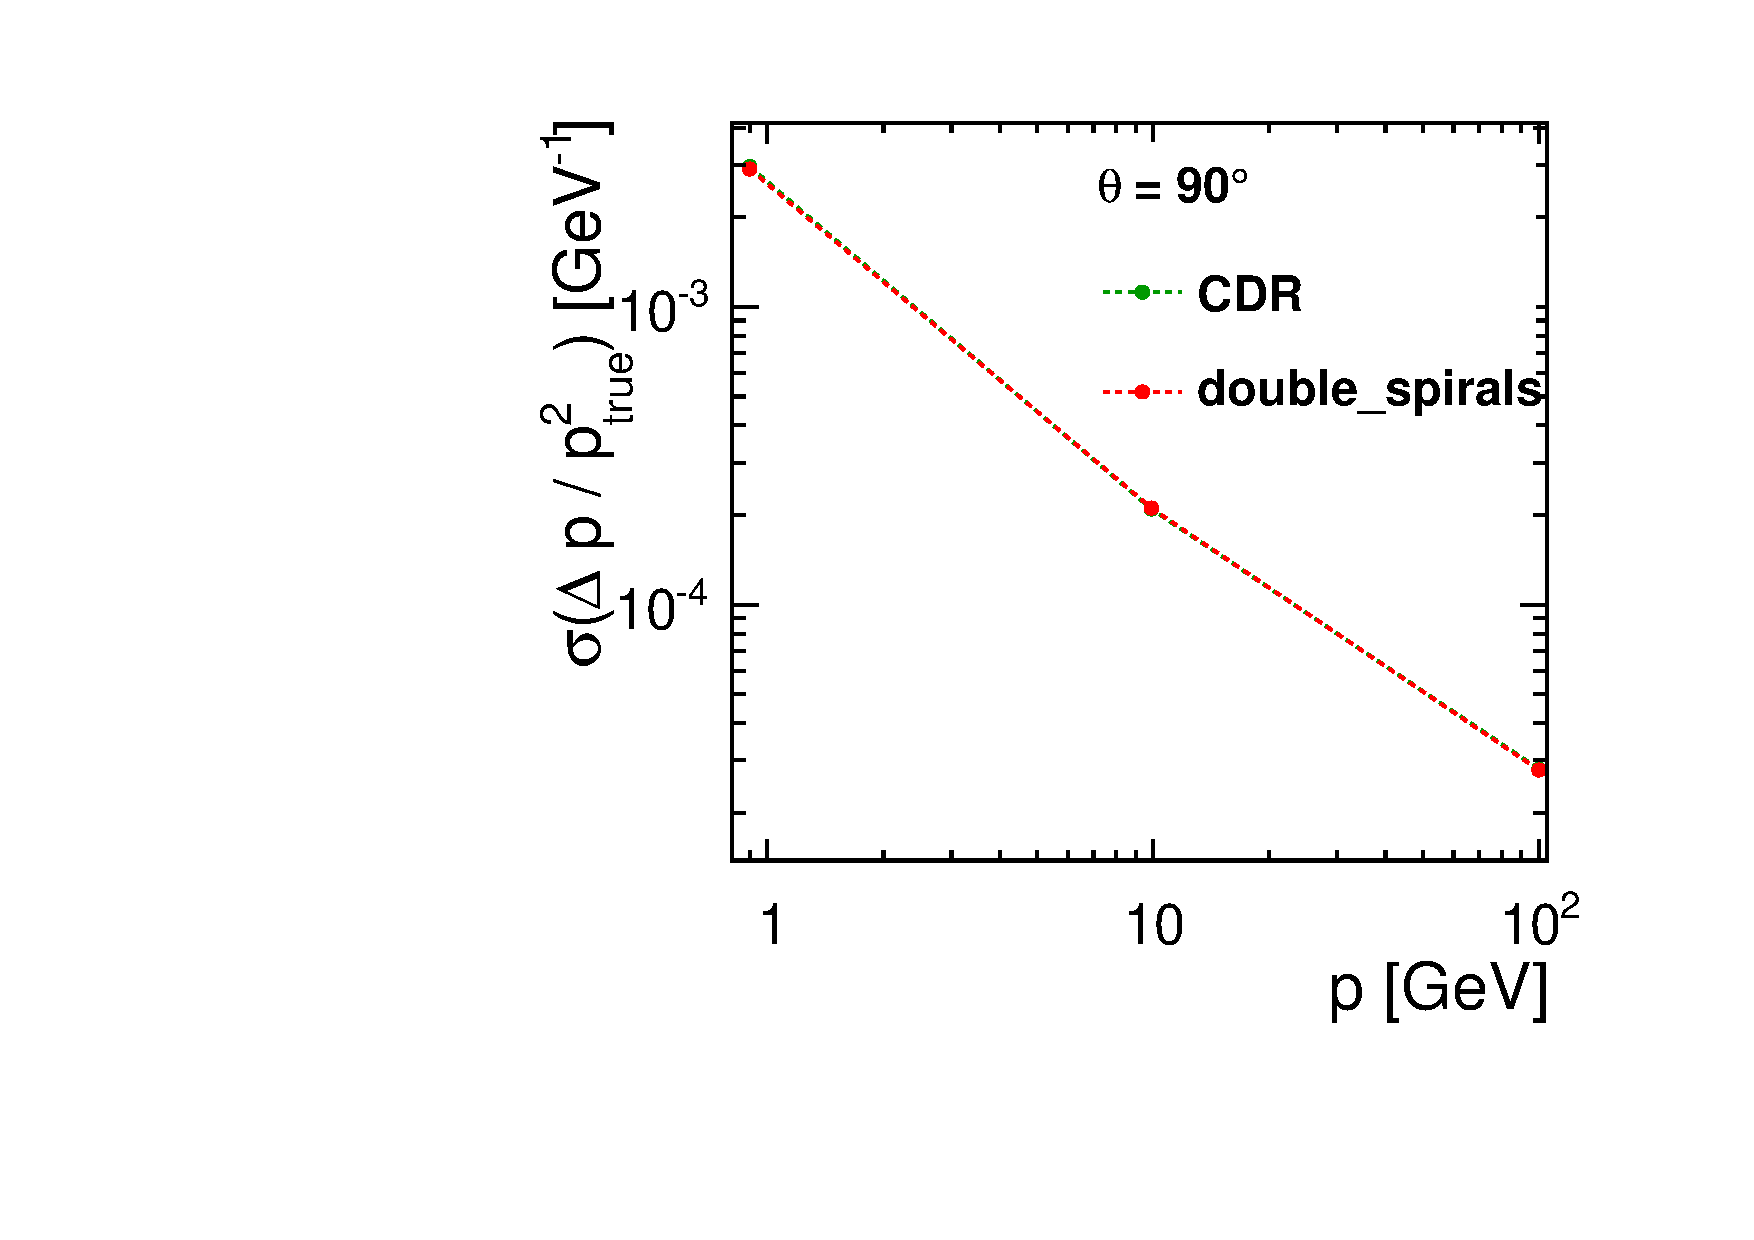
\includegraphics[width=\textwidth]{Figures/Geometries/pT_resolution_double.pdf}
          \caption{Momentum resolution}
          \label{}
        \end{subfigure}%
        ~ 
        \begin{subfigure}[b]{0.4\textwidth}
          \centering
          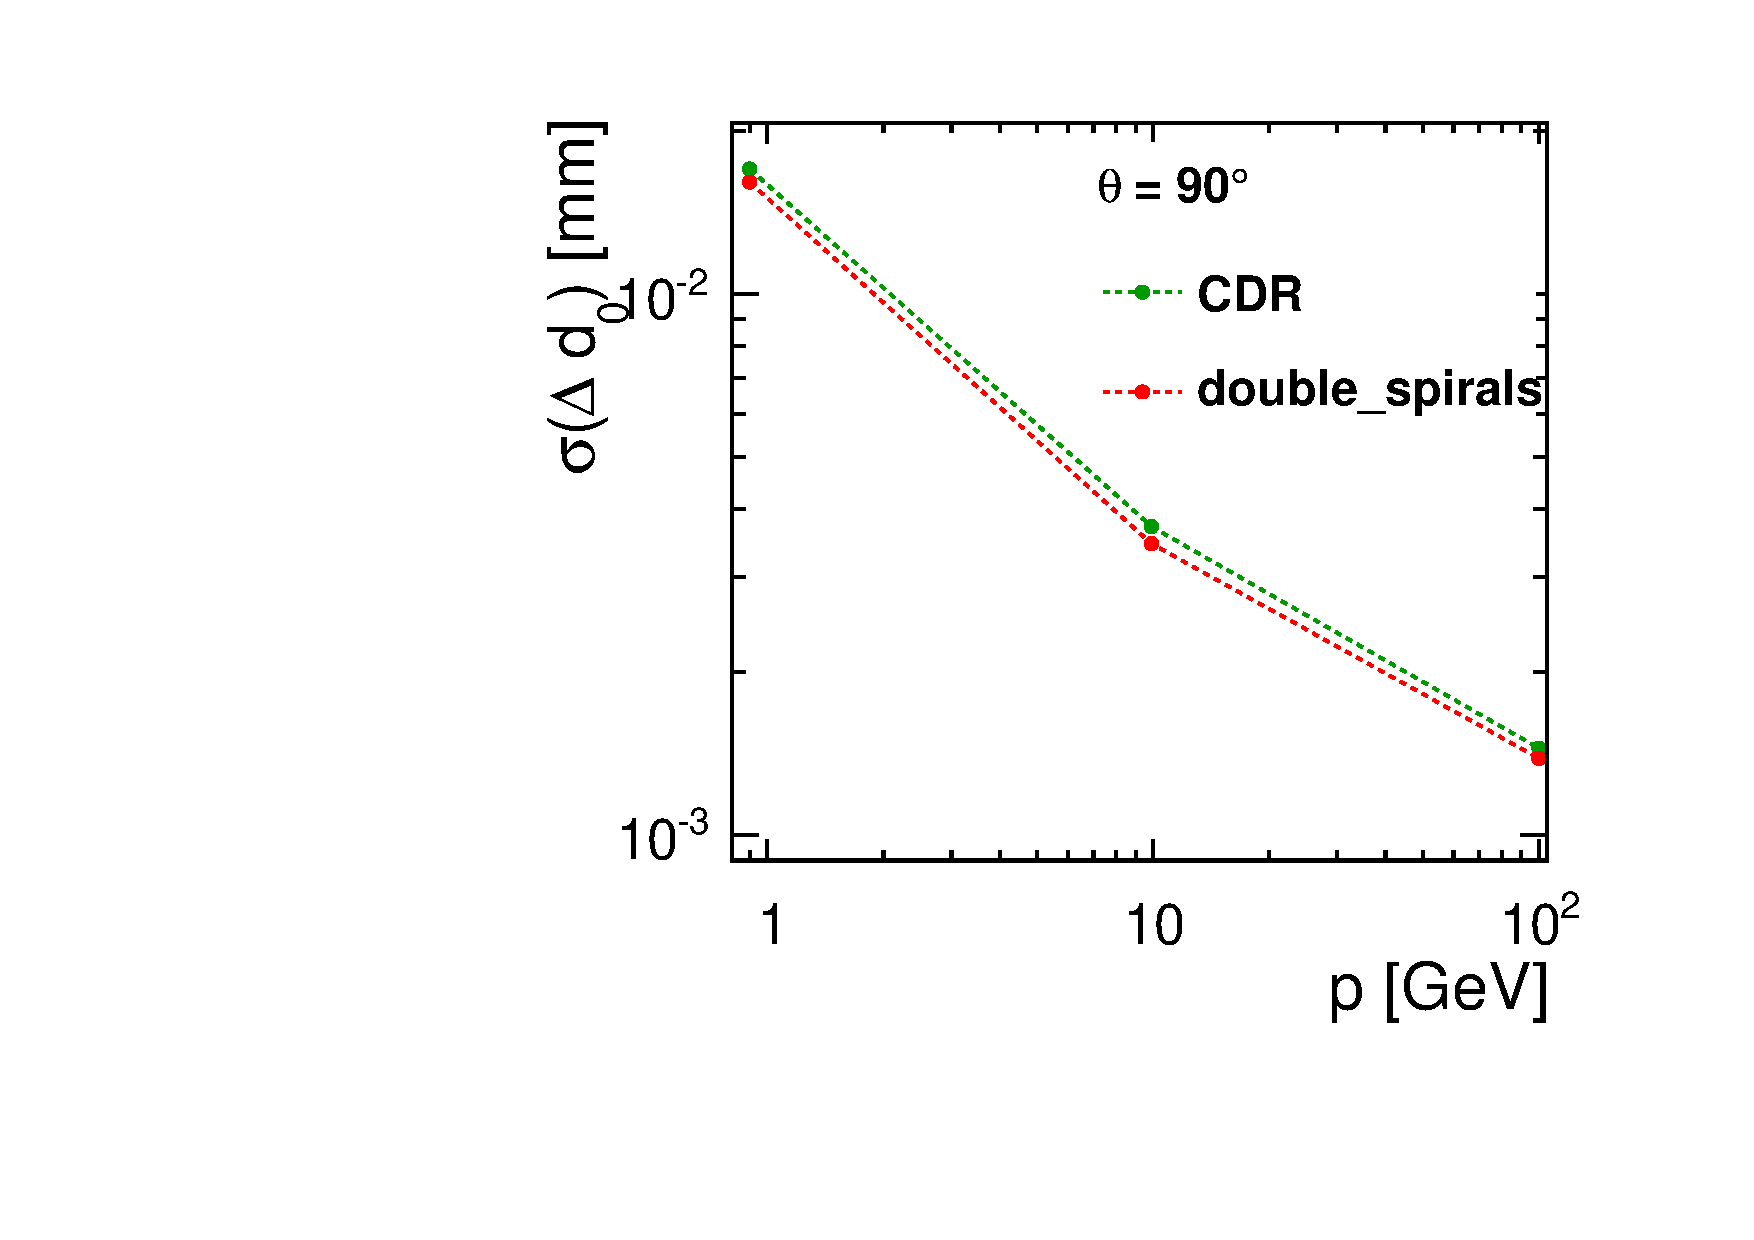
\includegraphics[width=\textwidth]{Figures/Geometries/d0_resolution_double.pdf}
          \caption{Transverse impact-parameter resolution}
          \label{}
        \end{subfigure}
        ~
        \begin{subfigure}[b]{\textwidth}
          \centering
          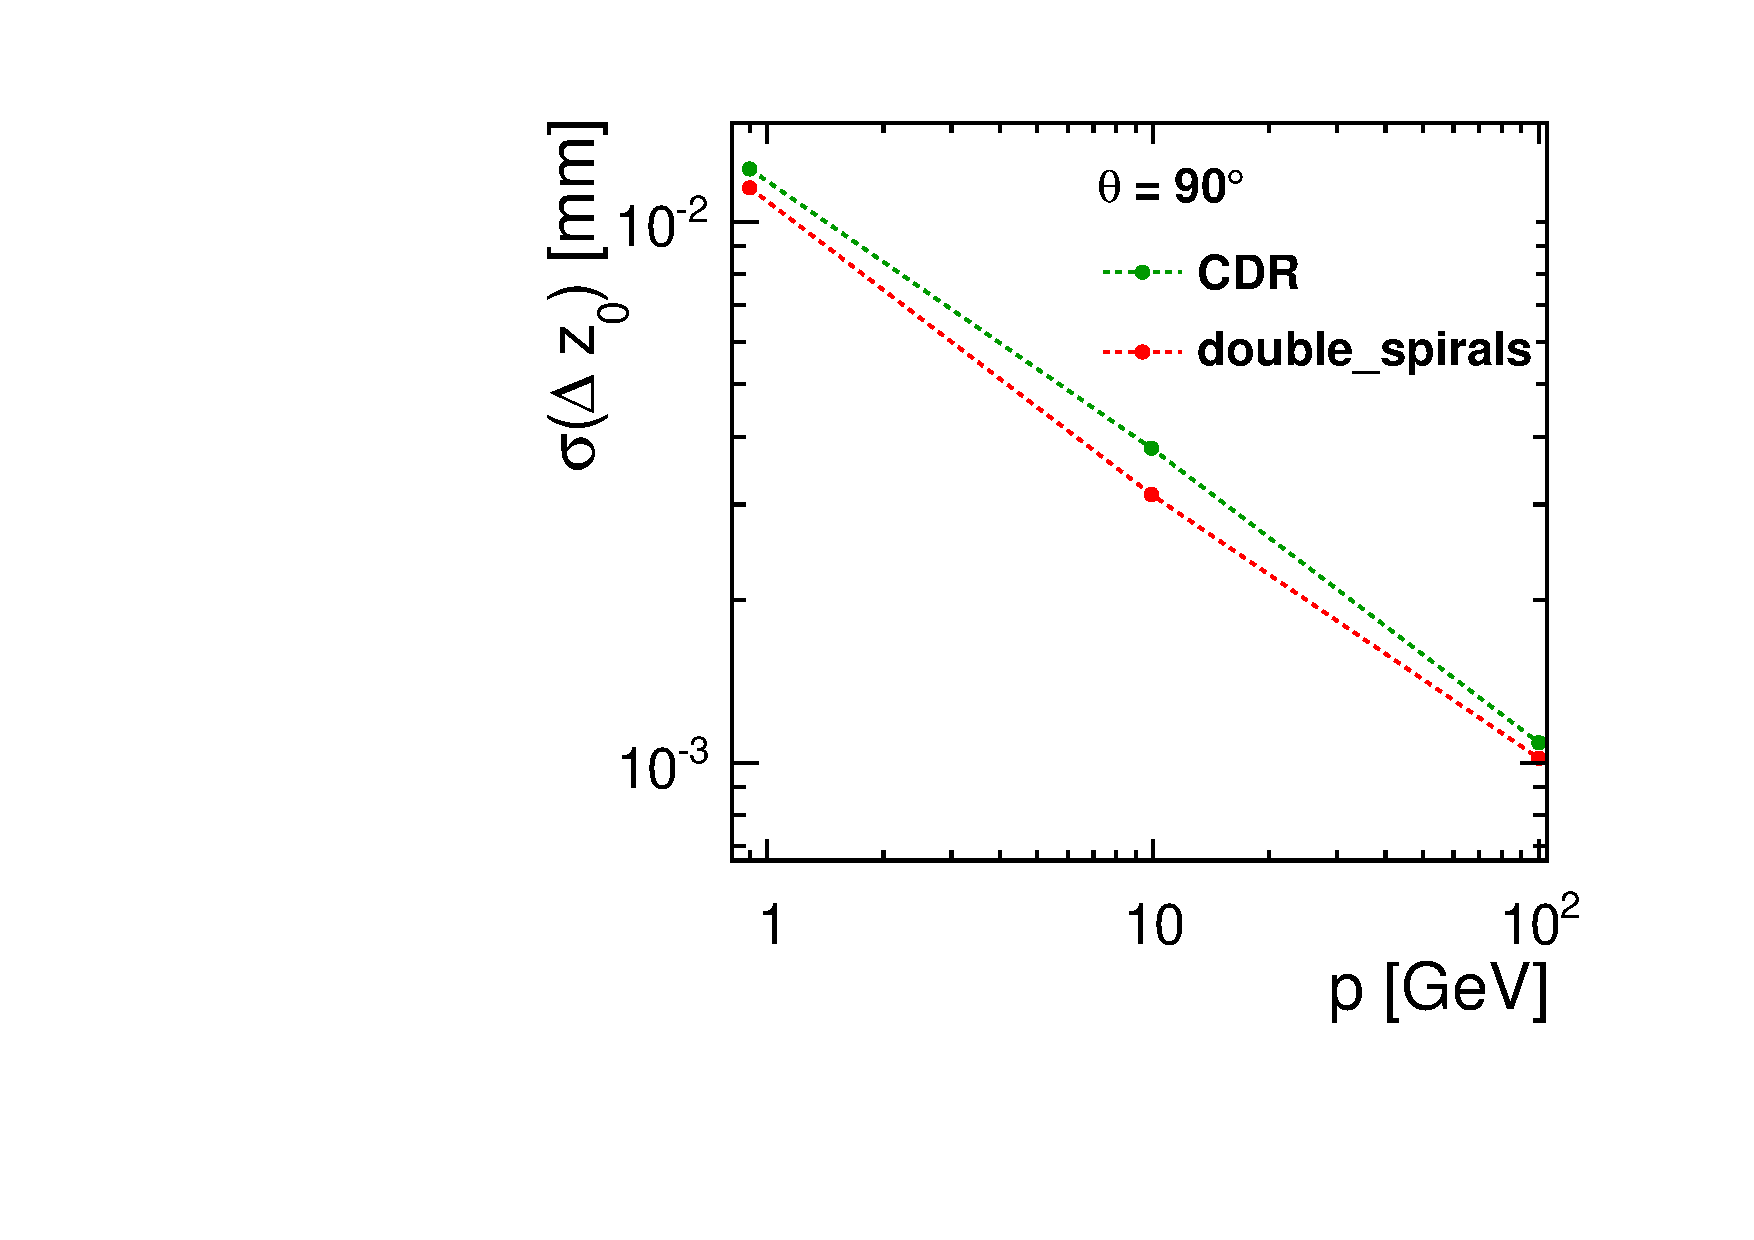
\includegraphics[width=0.4\textwidth]{Figures/Geometries/z0_resolution_double.pdf}
          \caption{Longitudinal impact-parameter resolution}
          \label{}
        \end{subfigure}
        \caption{(a) Momentum, (b) transverse impact-parameter and
          (c) longitudinal impact-parameter resolutions for the CDR and
          the {\it double\_spirals} geometries for singles muons at $\theta = 90^\circ$.}\label{fig:doubleLayerRes}
\end{figure}

We can conclude that the use of double-layered modules with 6 sensors in the barrel slightly improves the $d_0$ and $z_0$ resolutions, compared to the geometry with 5 single layers (CDR and \textit{spirals} geometries).

\newpage

\subsection{The \emph{double\_spirals\_v2} geometry}
The impact of the \begin{it}double\_spirals\_v2\end{it} geometry on the tracking performance is studied in the barrel and the endcap regions using single muons with polar angles of $\theta=90^{\circ}$ and $\theta=20^{\circ}$ in Figures~\ref{fig:doubleSpiralsV2Res90} and \ref{fig:doubleSpiralsV2Res20}, respectively. For muons at $\theta=20^{\circ}$, two different azimuthal angles $\phi=180^{\circ}$ and $\phi=225^{\circ}$ are considered which correspond to the first and the last module of the first endcap layer.
The impact of the material budget on the transverse and longitudinal impact-parameter resolutions is more visible in the barrel region.

\begin{figure}[H]
        \centering
        \begin{subfigure}[b]{0.5\textwidth}
          \centering
          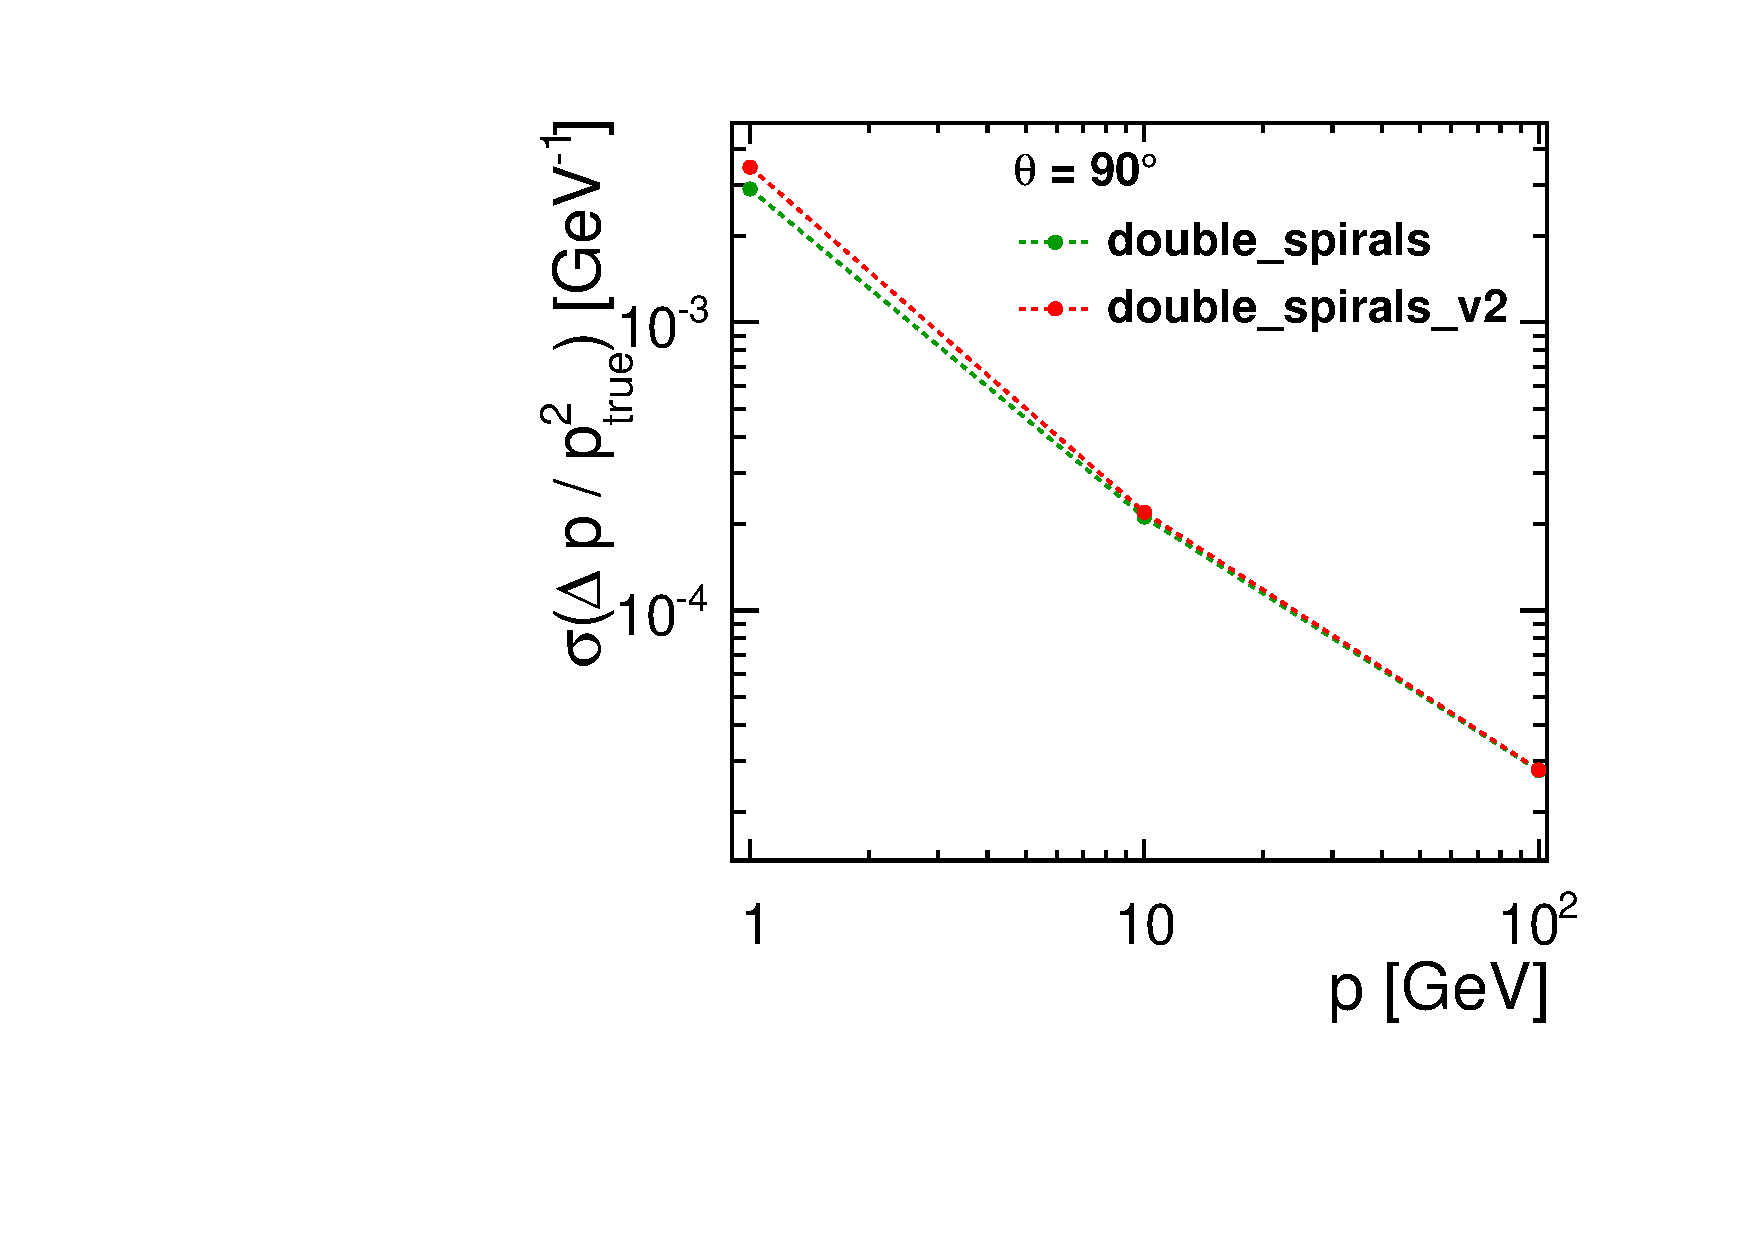
\includegraphics[width=\textwidth]{Figures/Geometries/p_resolution_double_spirals_v2_theta90.pdf}
          \caption{Momentum resolution}
          \label{}
        \end{subfigure}%
        ~ 
        \begin{subfigure}[b]{0.5\textwidth}
          \centering
          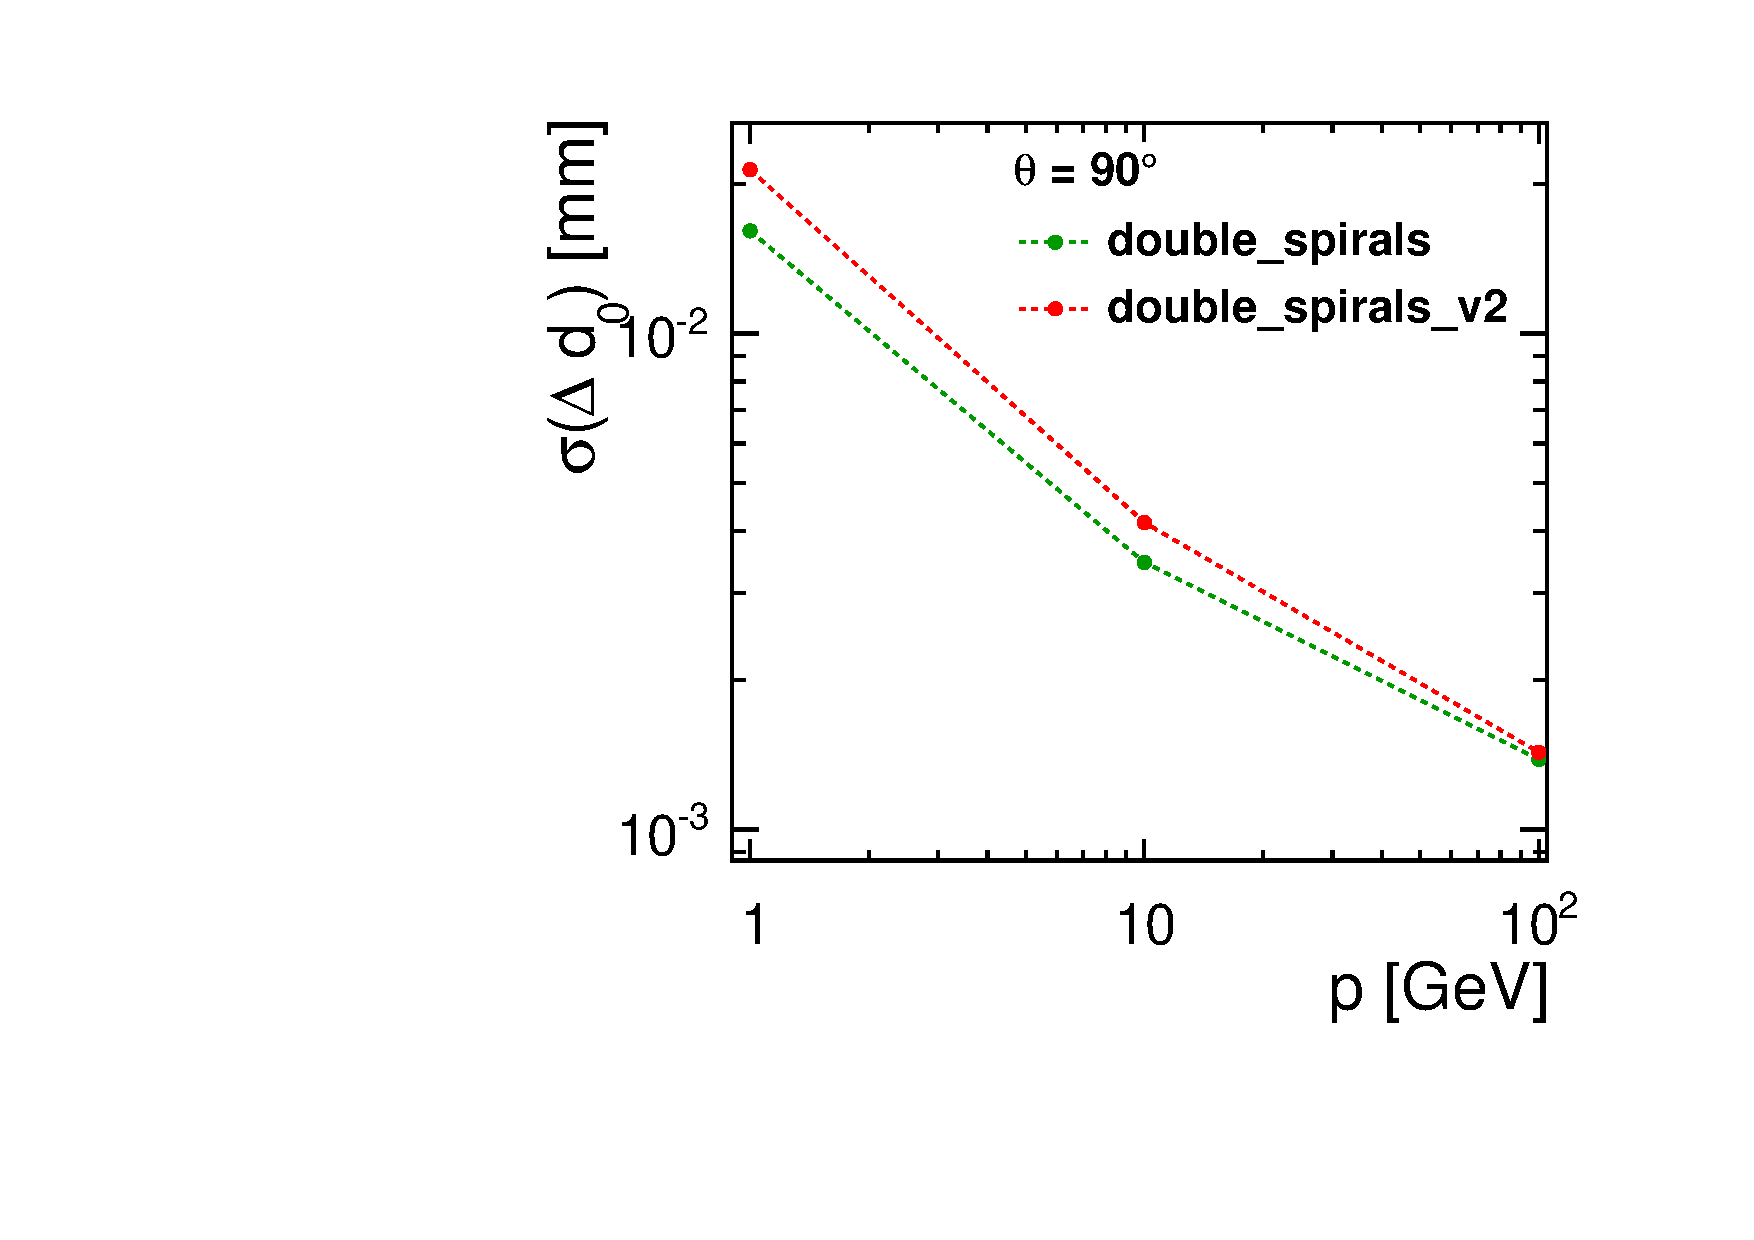
\includegraphics[width=\textwidth]{Figures/Geometries/d0_resolution_double_spirals_v2_theta90.pdf}
          \caption{Transverse impact-parameter resolution}
          \label{}
        \end{subfigure}
        ~
        \begin{subfigure}[b]{\textwidth}
          \centering
          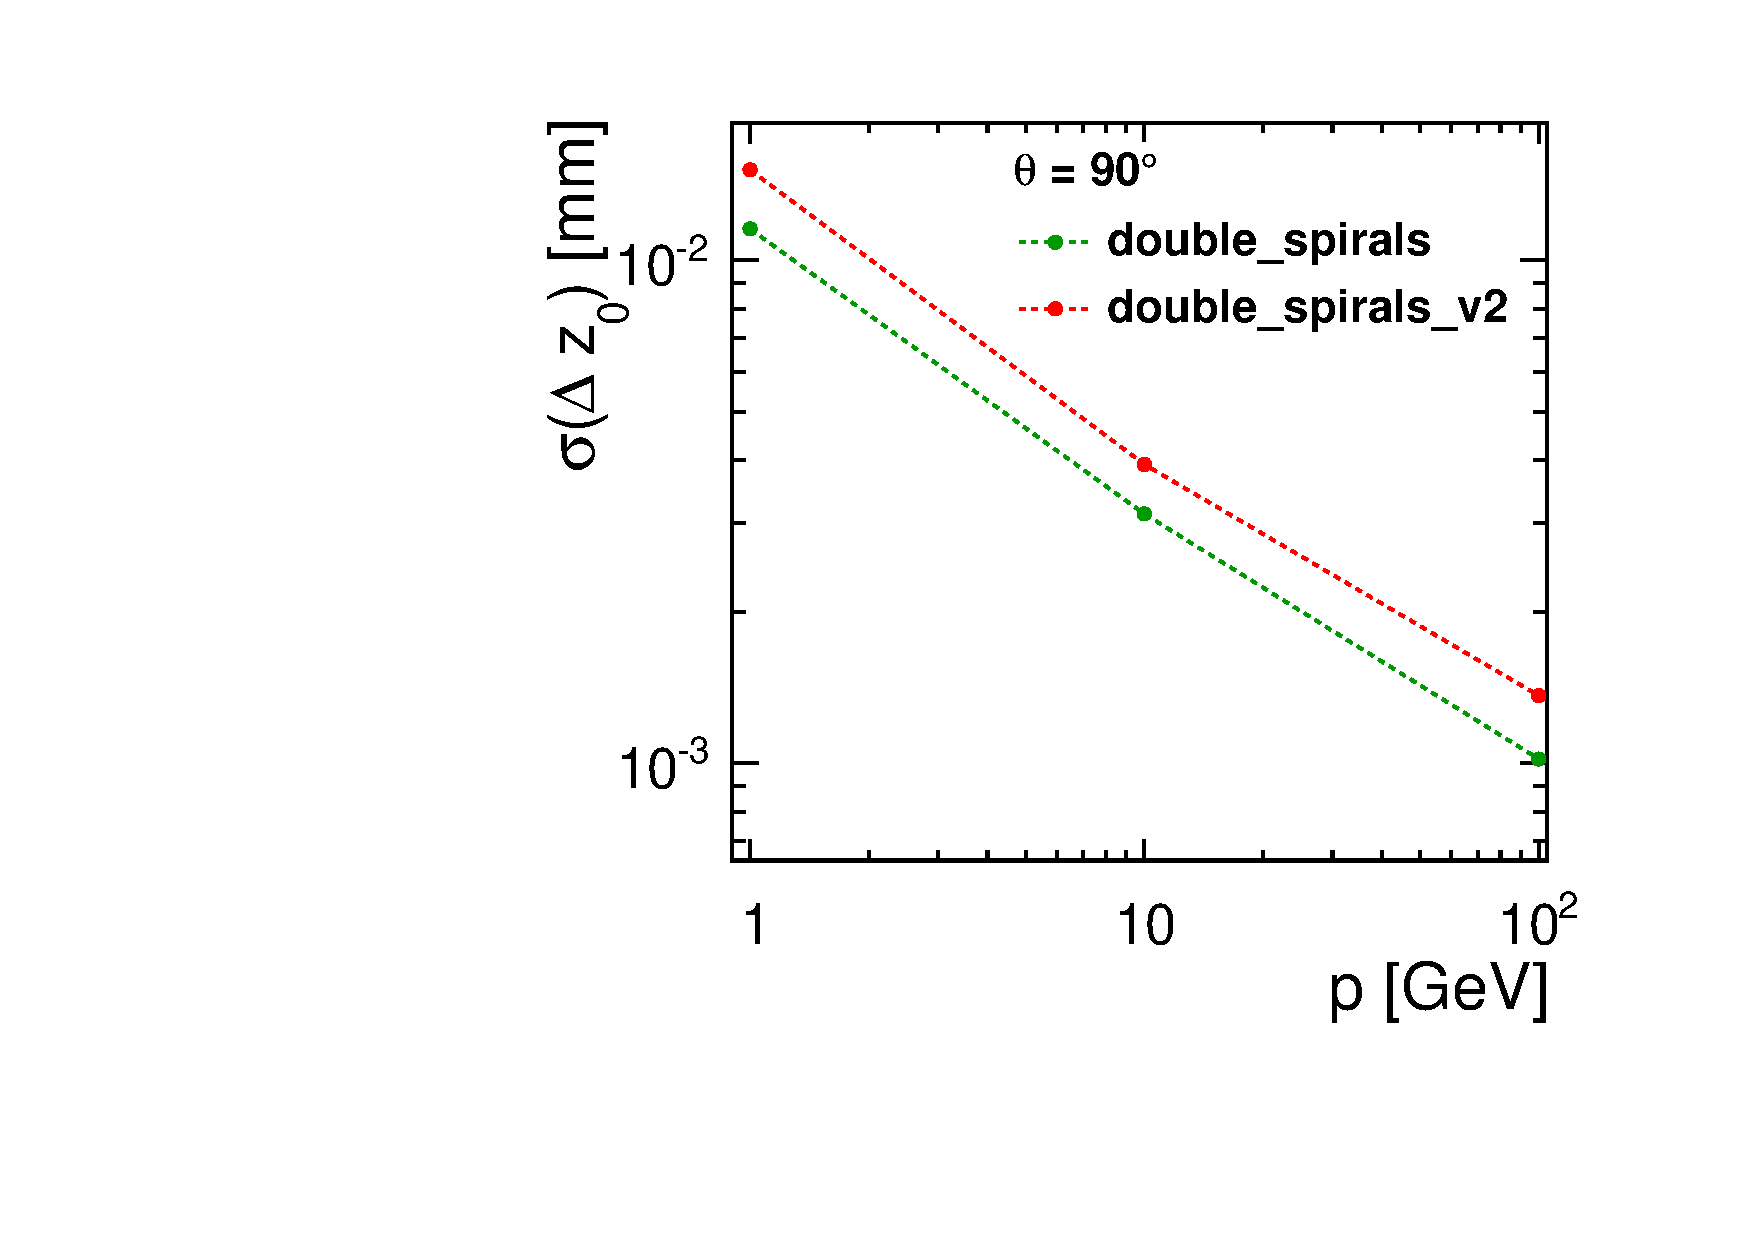
\includegraphics[width=0.5\textwidth]{Figures/Geometries/z0_resolution_double_spirals_v2_theta90.pdf}
          \caption{Longitudinal impact-parameter resolution}
          \label{}
        \end{subfigure}
        \caption{(a) Momentum, (b) transverse impact-parameter and
          (c) longitudinal impact-parameter resolutions for the {\it
            double\_spirals} and the {\it double\_spirals\_v2} geometries for singles muons at $\theta = 90^\circ$.}\label{fig:doubleSpiralsV2Res90}
\end{figure}

\begin{figure}[H]
        \centering
        \begin{subfigure}[b]{0.5\textwidth}
          \centering
          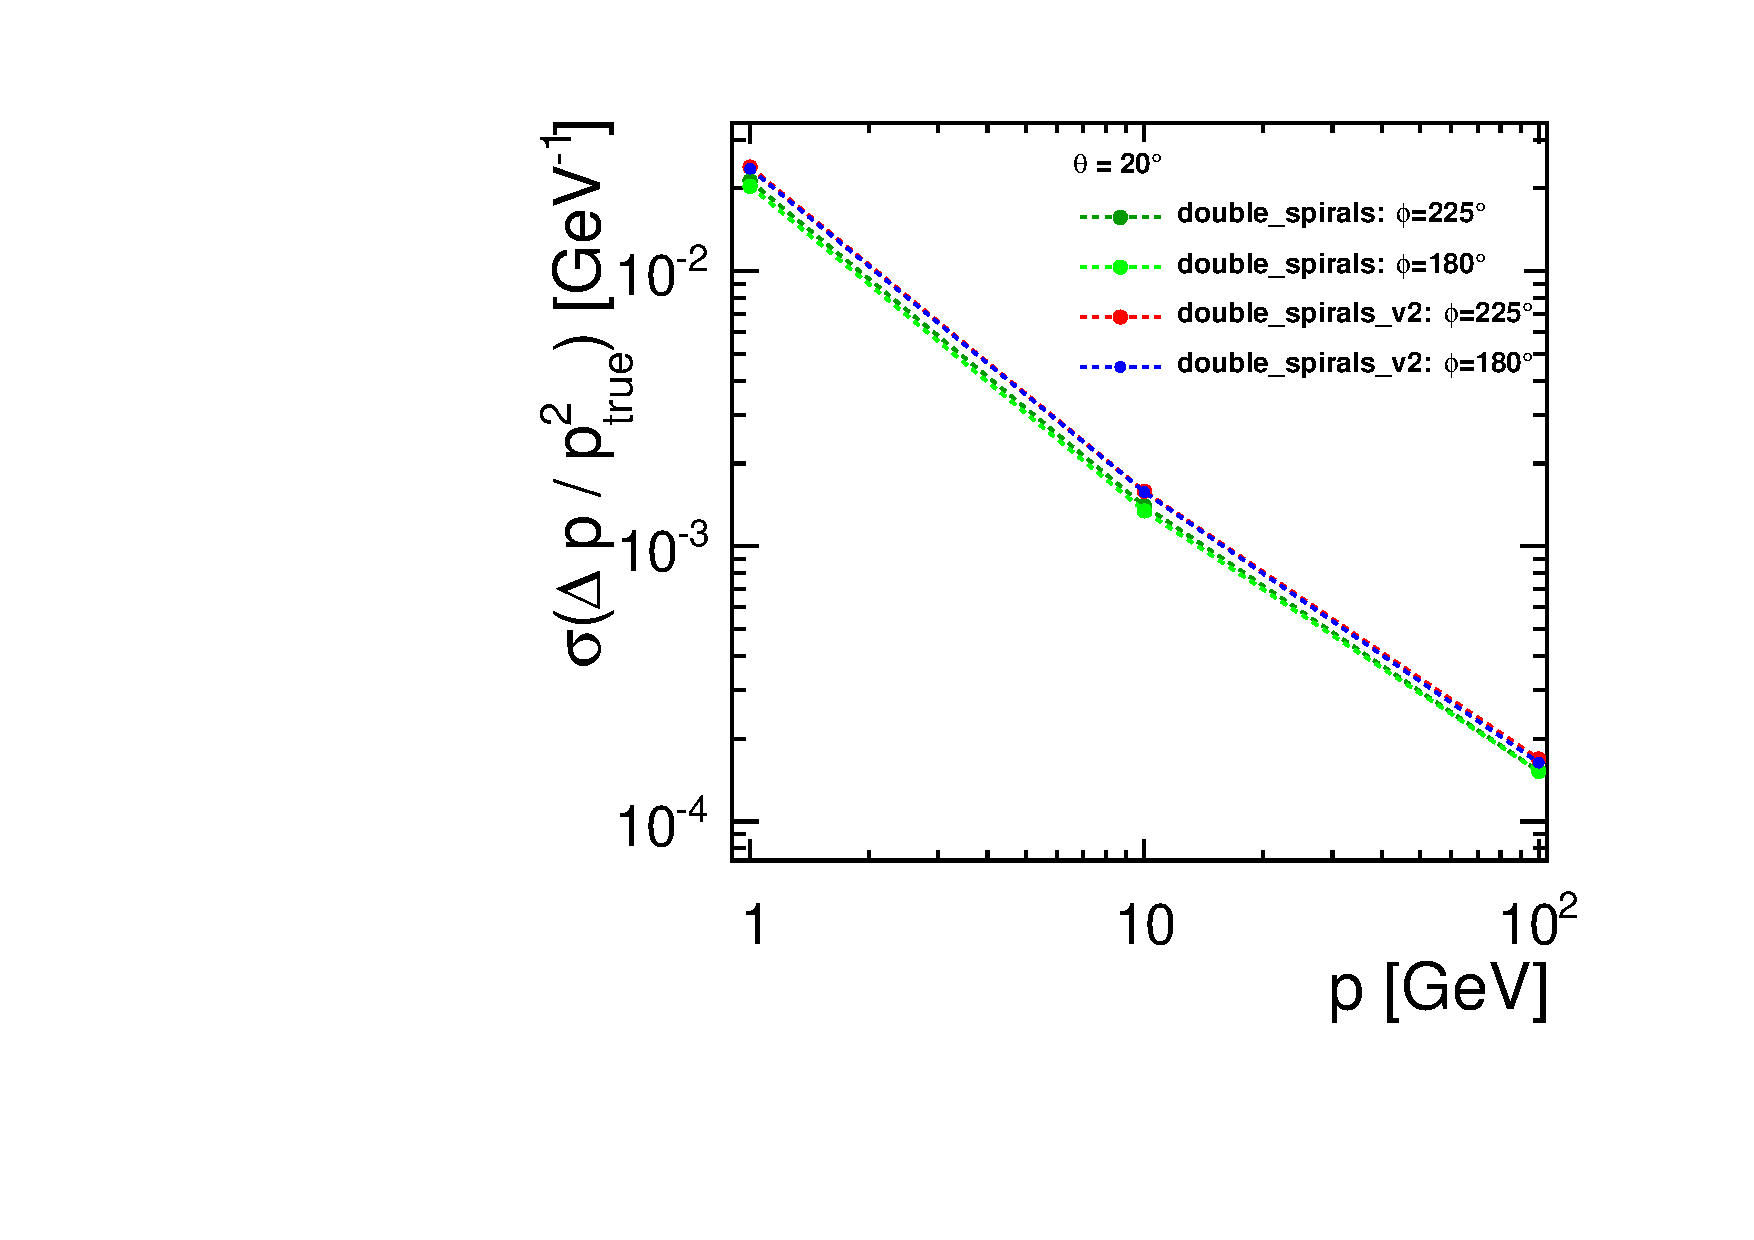
\includegraphics[width=\textwidth]{Figures/Geometries/p_resolution_double_spirals_v2_theta20.pdf}
          \caption{Momentum resolution}
          \label{}
        \end{subfigure}%
        ~ 
        \begin{subfigure}[b]{0.5\textwidth}
          \centering
          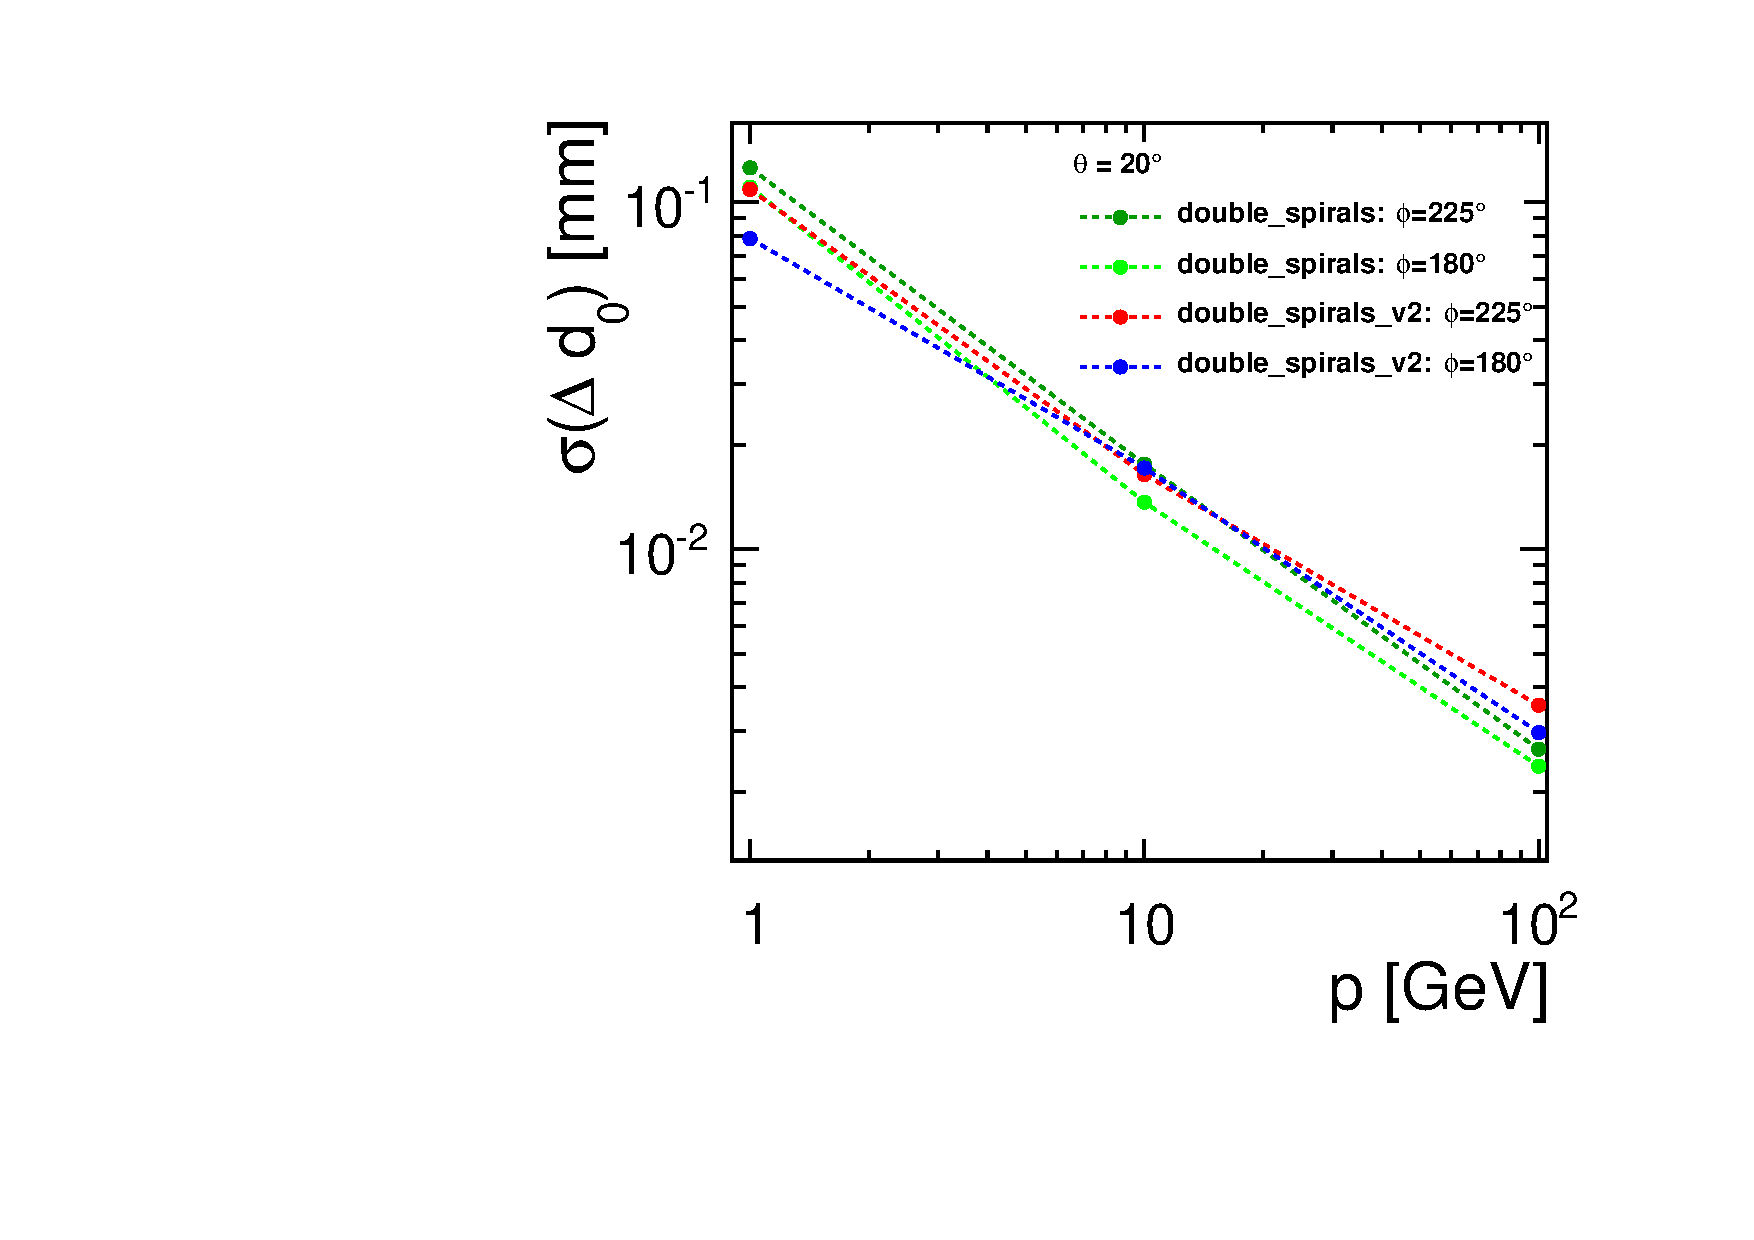
\includegraphics[width=\textwidth]{Figures/Geometries/d0_resolution_double_spirals_v2_theta20.pdf}
          \caption{Transverse impact-parameter resolution}
          \label{}
        \end{subfigure}
        ~
        \begin{subfigure}[b]{\textwidth}
          \centering
          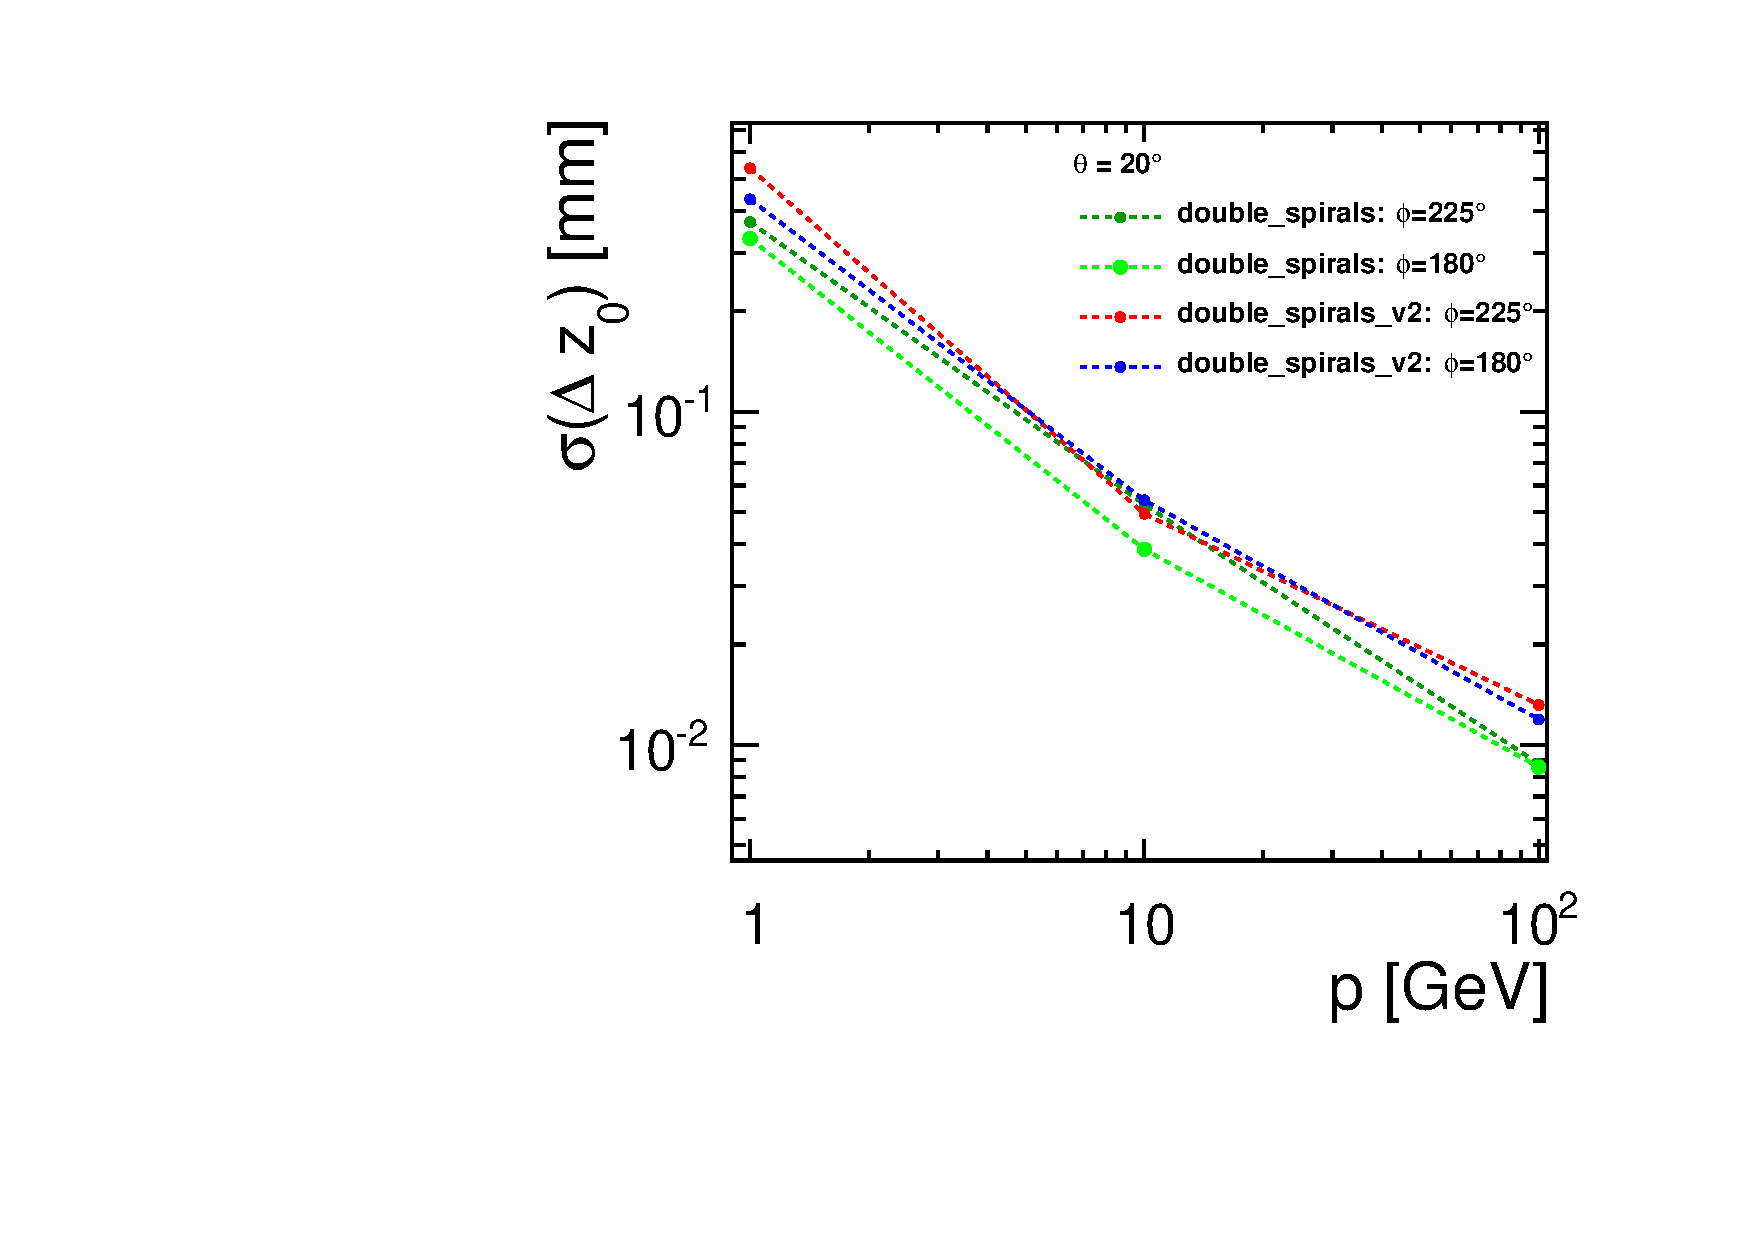
\includegraphics[width=0.5\textwidth]{Figures/Geometries/z0_resolution_double_spirals_v2_theta20.pdf}
          \caption{Longitudinal impact-parameter resolution}
          \label{}
        \end{subfigure}
        \caption{(a) Momentum, (b) transverse impact-parameter and
          (c) longitudinal impact-parameter resolutions for the
          {\it double\_spirals} and the {\it double\_spirals\_v2} geometries for
          singles muons at $\theta = 20^\circ$ with azimuthal angles
          of  $\phi = 225^\circ$ or $\phi = 180^\circ$.}\label{fig:doubleSpiralsV2Res20}
\end{figure}

%
\newpage
\section{Flavour-tagging performance}\label{sec:impactOfGeometries}

The different geometries described in Section~\ref{sec:Geometries} are compared based on their flavour-tagging performance. The flavour tagging is studied using the LCFIPlus package~\cite{website:LCFIPlus}. \\
The performance of the flavour tagging depends on the jet energy and polar angle. For this reason, the study is done considering dijet events with center-of-mass energies, $\sqrt{s}$, of 91~GeV, 200~GeV, 500~GeV and 1000~GeV having polar angles of $\theta=10^\circ, 20^\circ, ..., 90^\circ$ with a uniform distribution in $\phi$ angles. Initial state radiation (ISR) and beamstrahlung (BS) were switched off during the event generation and hence the final-state quarks are in a back-to-back configuration.\\
For each jet flavour, energy and angle, 80000 events are used for the following processes:
\begin{itemize}
\item e$^+$e$^-$ $\rightarrow$ b\={b}
\item e$^+$e$^-$ $\rightarrow$ c\={c}
\item e$^+$e$^-$ $\rightarrow$ u\={u}
\item e$^+$e$^-$ $\rightarrow$ d\={d}
\item e$^+$e$^-$ $\rightarrow$ s\={s}
\end{itemize}

The boosted decision trees (BDTs) are trained using 50\% of the generated events and the other 50\% are used for testing the performance of the flavour tagging.
%% The software versions used are given in Table \ref{tab:softwareVersions}:

%% \begin{table}[H]
%%   \caption{Software versions used for the flavour tagging.}
%%   \begin{center}
%%     \begin{tabular}{ c c}
%%       \hline
%%       Software & Version \\ \hline \hline
%%       SLIC & v3r0p3 \\ \hline
%%       org.lcsim & 2.5 \\ \hline
%%       LCFIPlus & v0.52 \\ \hline
%%     \end{tabular}
%%   \end{center}
%%   \label{tab:softwareVersions}
%% \end{table}

\subsection{Jet-energy dependence}
The dependence of the flavour-tagging performance on the jet energy is shown in Figures \ref{fig:FTEnergyDependenceB} and \ref{fig:FTEnergyDependenceC} using the \begin{it}spirals\end{it} geometry and dijet events at different center-of-mass energies with a mixture of all considered polar angles. \\
In Figure~\ref{fig:FTEnergyDependenceB}, the fake rate of recognising charm and light flavour (LF) jets as beauty jets is plotted versus the b-tag efficiency. In Figure~\ref{fig:FTEnergyDependenceC}, the fake rate of recognising beauty and light flavour jets as charm jets is plotted versus the c-tag efficiency. \\
In general, the b-tag performance is better for jets with lower
energies. This can be explained by the fact that a B hadron with lower
energy has a shorter decay length and therefore decays most likely
before the first barrel layer of the vertex detector, while a B hadron with higher energy
decays sometimes after the first layer. This leads to a degradation of
the track reconstruction and thus the vertex finding and flavour
tagging for high-energy jets.

\begin{figure}[H]
        \begin{subfigure}[b]{0.5\textwidth}
          \centering
          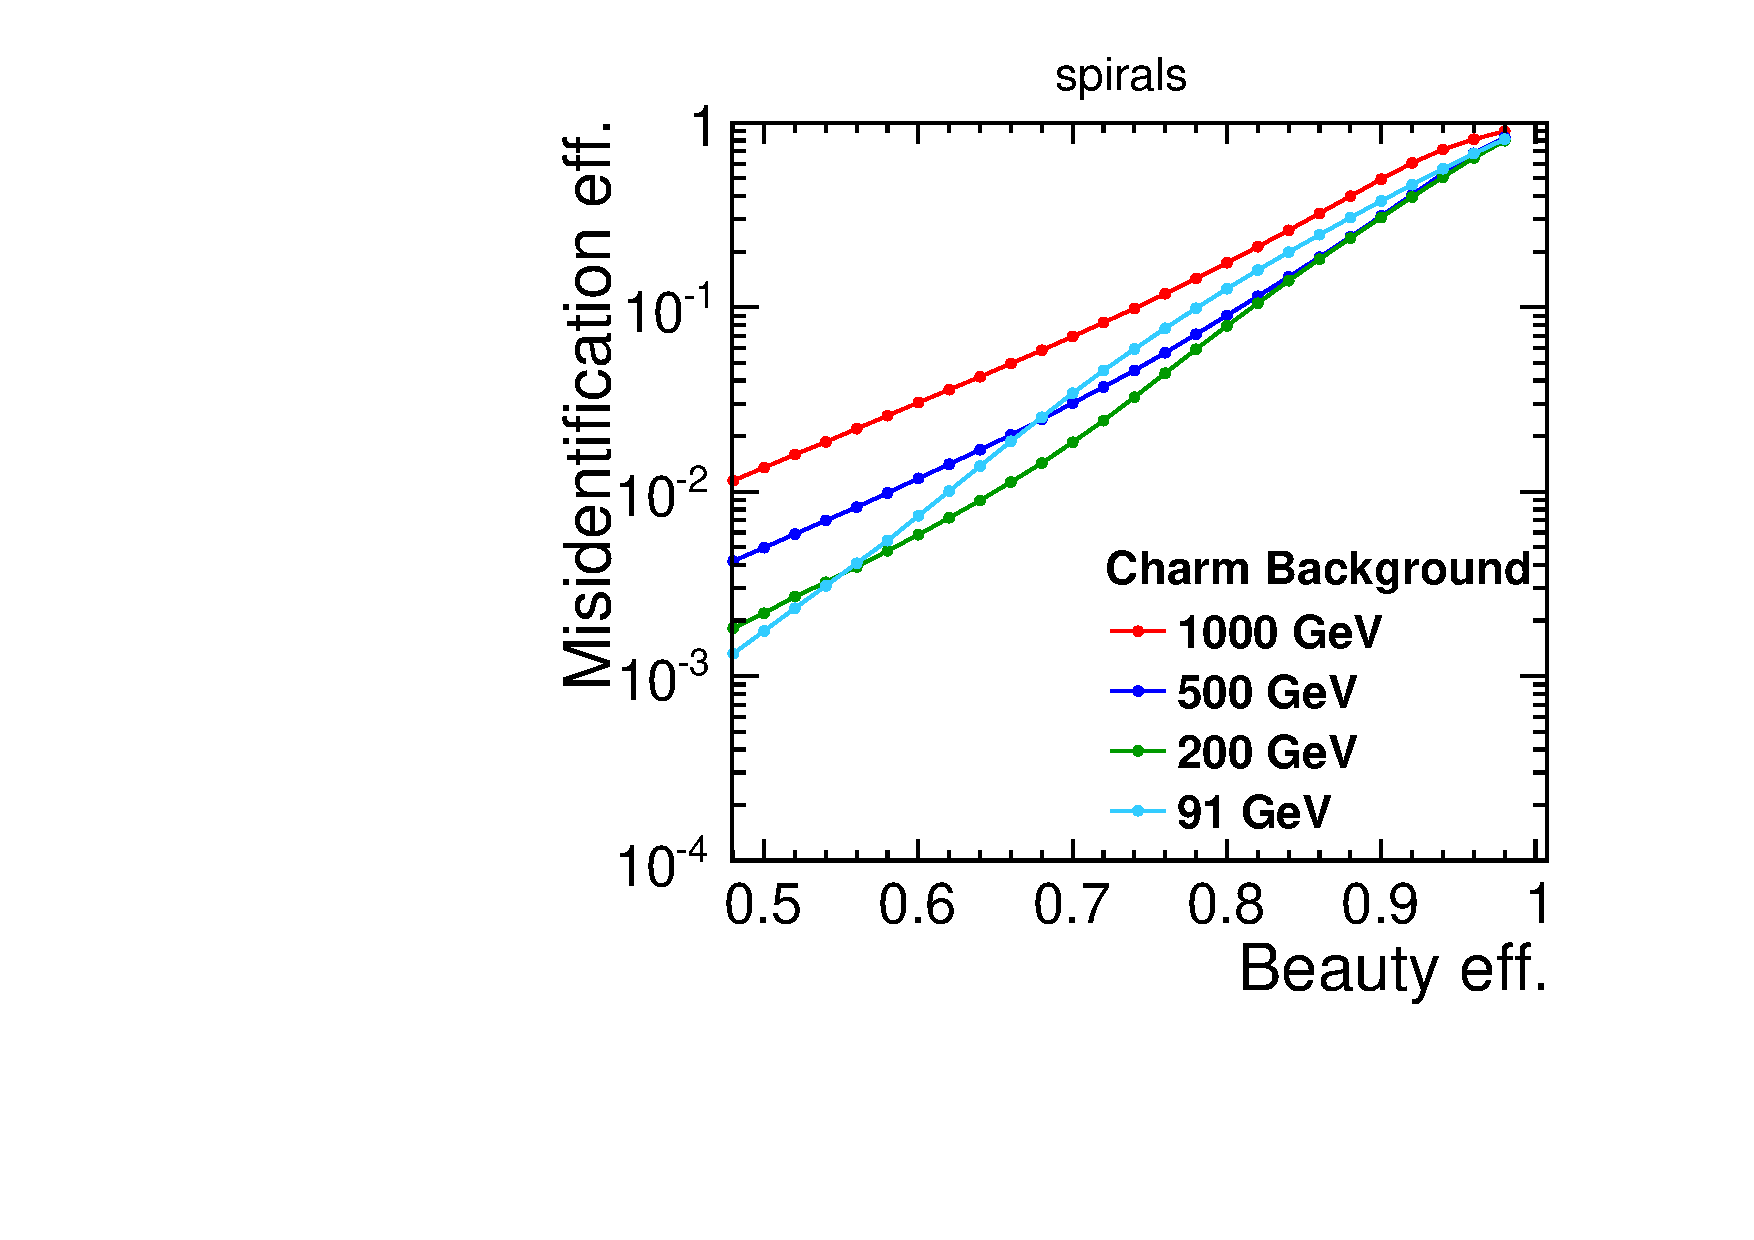
\includegraphics[width=\textwidth]{Figures/ImpactOfGeometries/Global_energies_CLIC_SiD_spirals_Beauty_Charm_.pdf}
          \caption{}
          \label{}
        \end{subfigure}%
        ~ 
        \begin{subfigure}[b]{0.5\textwidth}
          \centering
          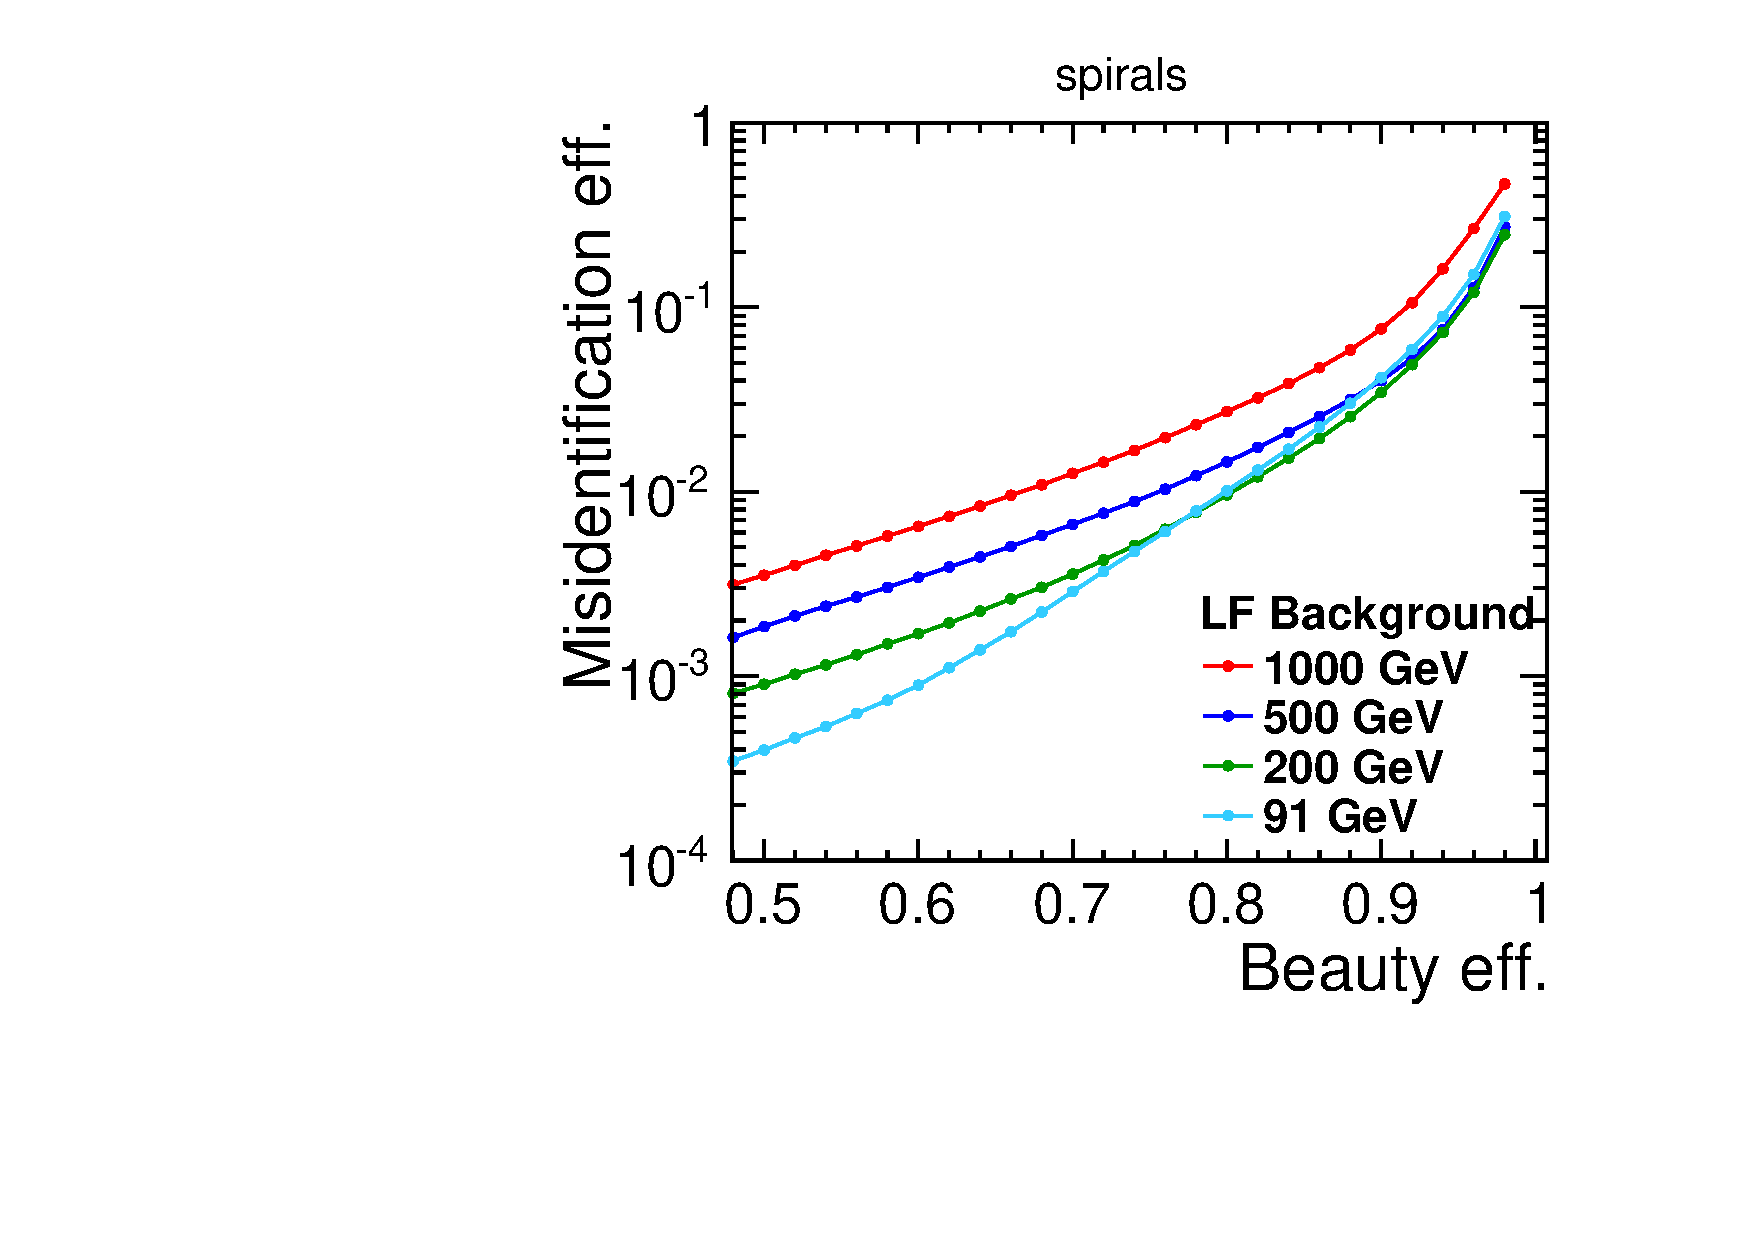
\includegraphics[width=\textwidth]{Figures/ImpactOfGeometries/Global_energies_CLIC_SiD_spirals_Beauty_LF_.pdf}
          \caption{}
          \label{}
        \end{subfigure}
        \caption{b-tag efficiencies and fake rates for dijets at a
          mixture of polar angles between $10^{\circ}$ and
          $90^{\circ}$ for the \textit{spirals} geometry. (a) shows the fake rate for recognising charm jets as beauty jets and (b) shows the fake rate for recognising light flavour jets as beauty jets.}\label{fig:FTEnergyDependenceB}
\end{figure}

\begin{figure}[H]
        \begin{subfigure}[b]{0.5\textwidth}
          \centering
          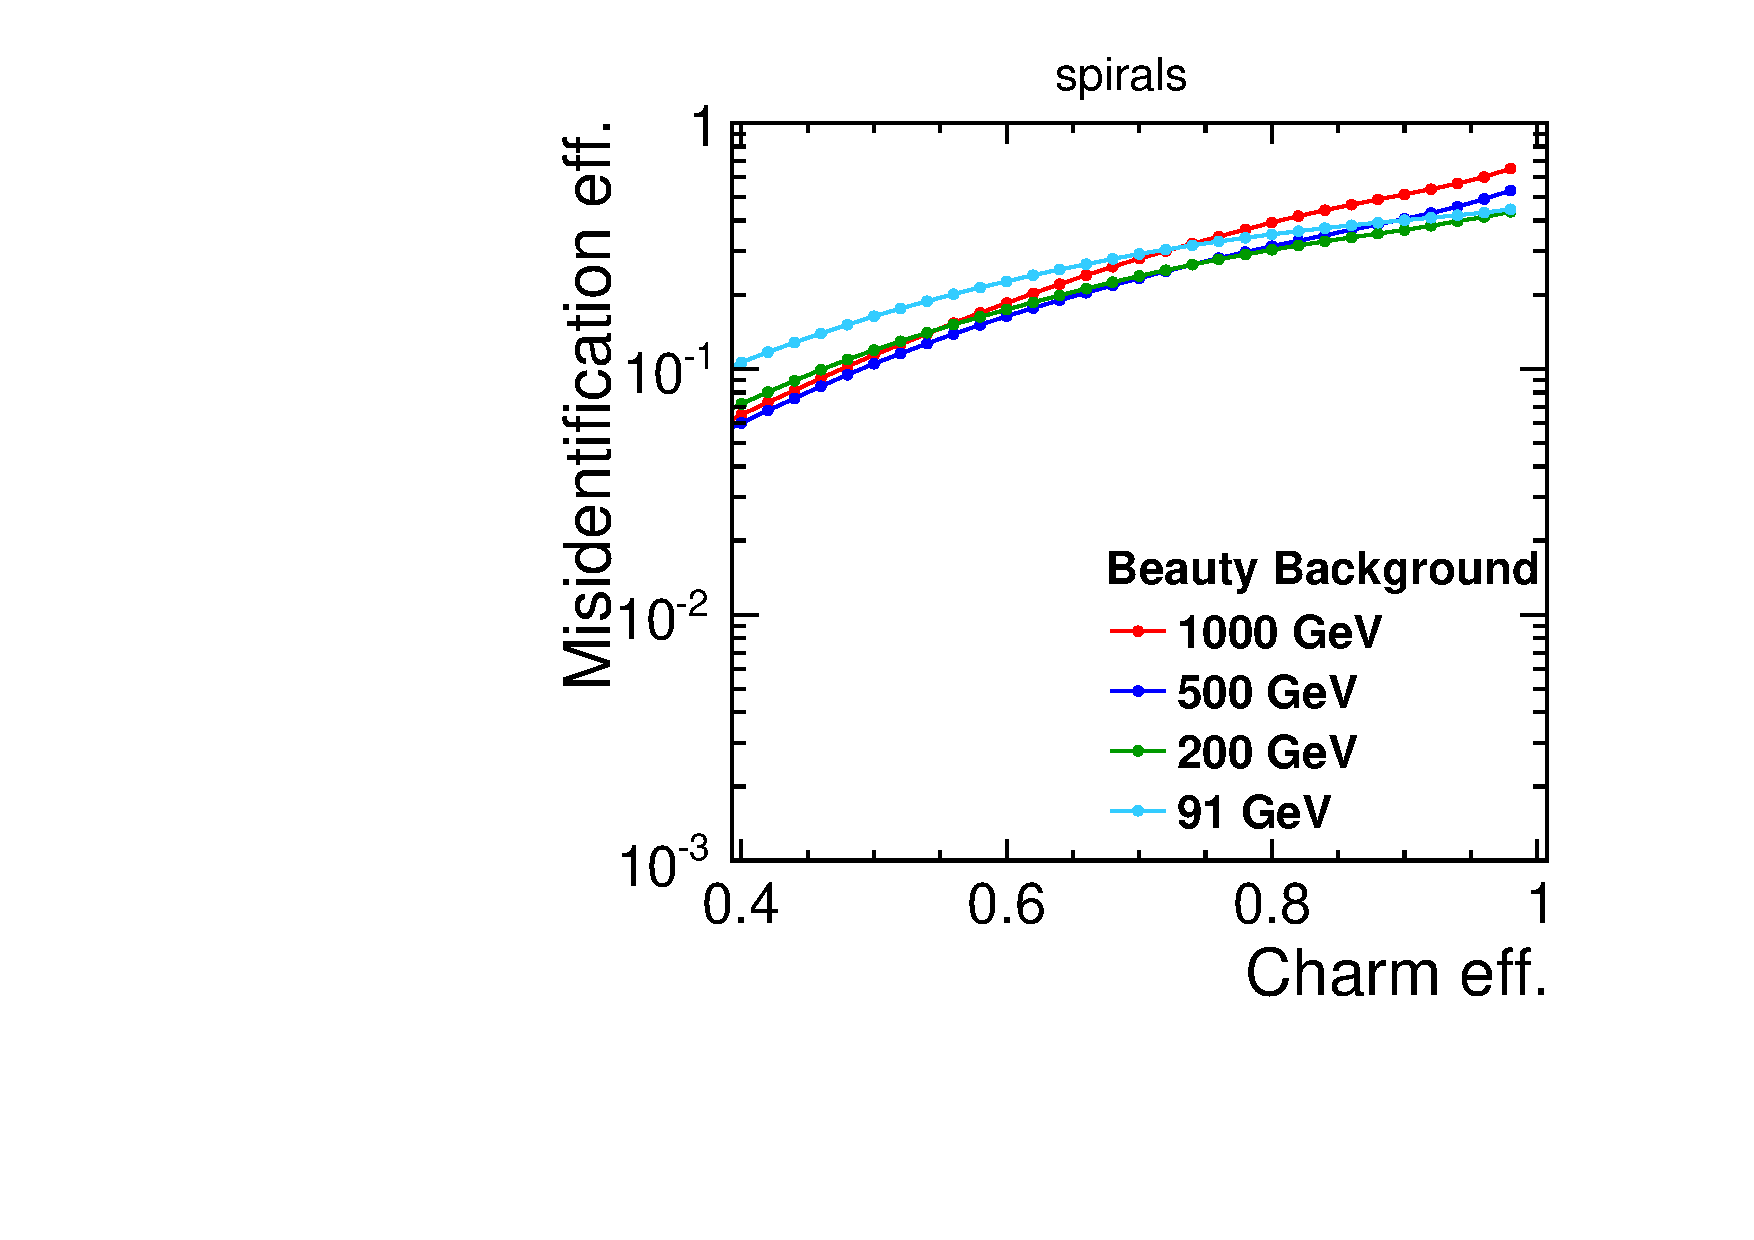
\includegraphics[width=\textwidth]{Figures/ImpactOfGeometries/Global_energies_CLIC_SiD_spirals_Charm_Beauty_.pdf}
          \caption{}
          \label{}
        \end{subfigure}%
        ~ 
        \begin{subfigure}[b]{0.5\textwidth}
          \centering
          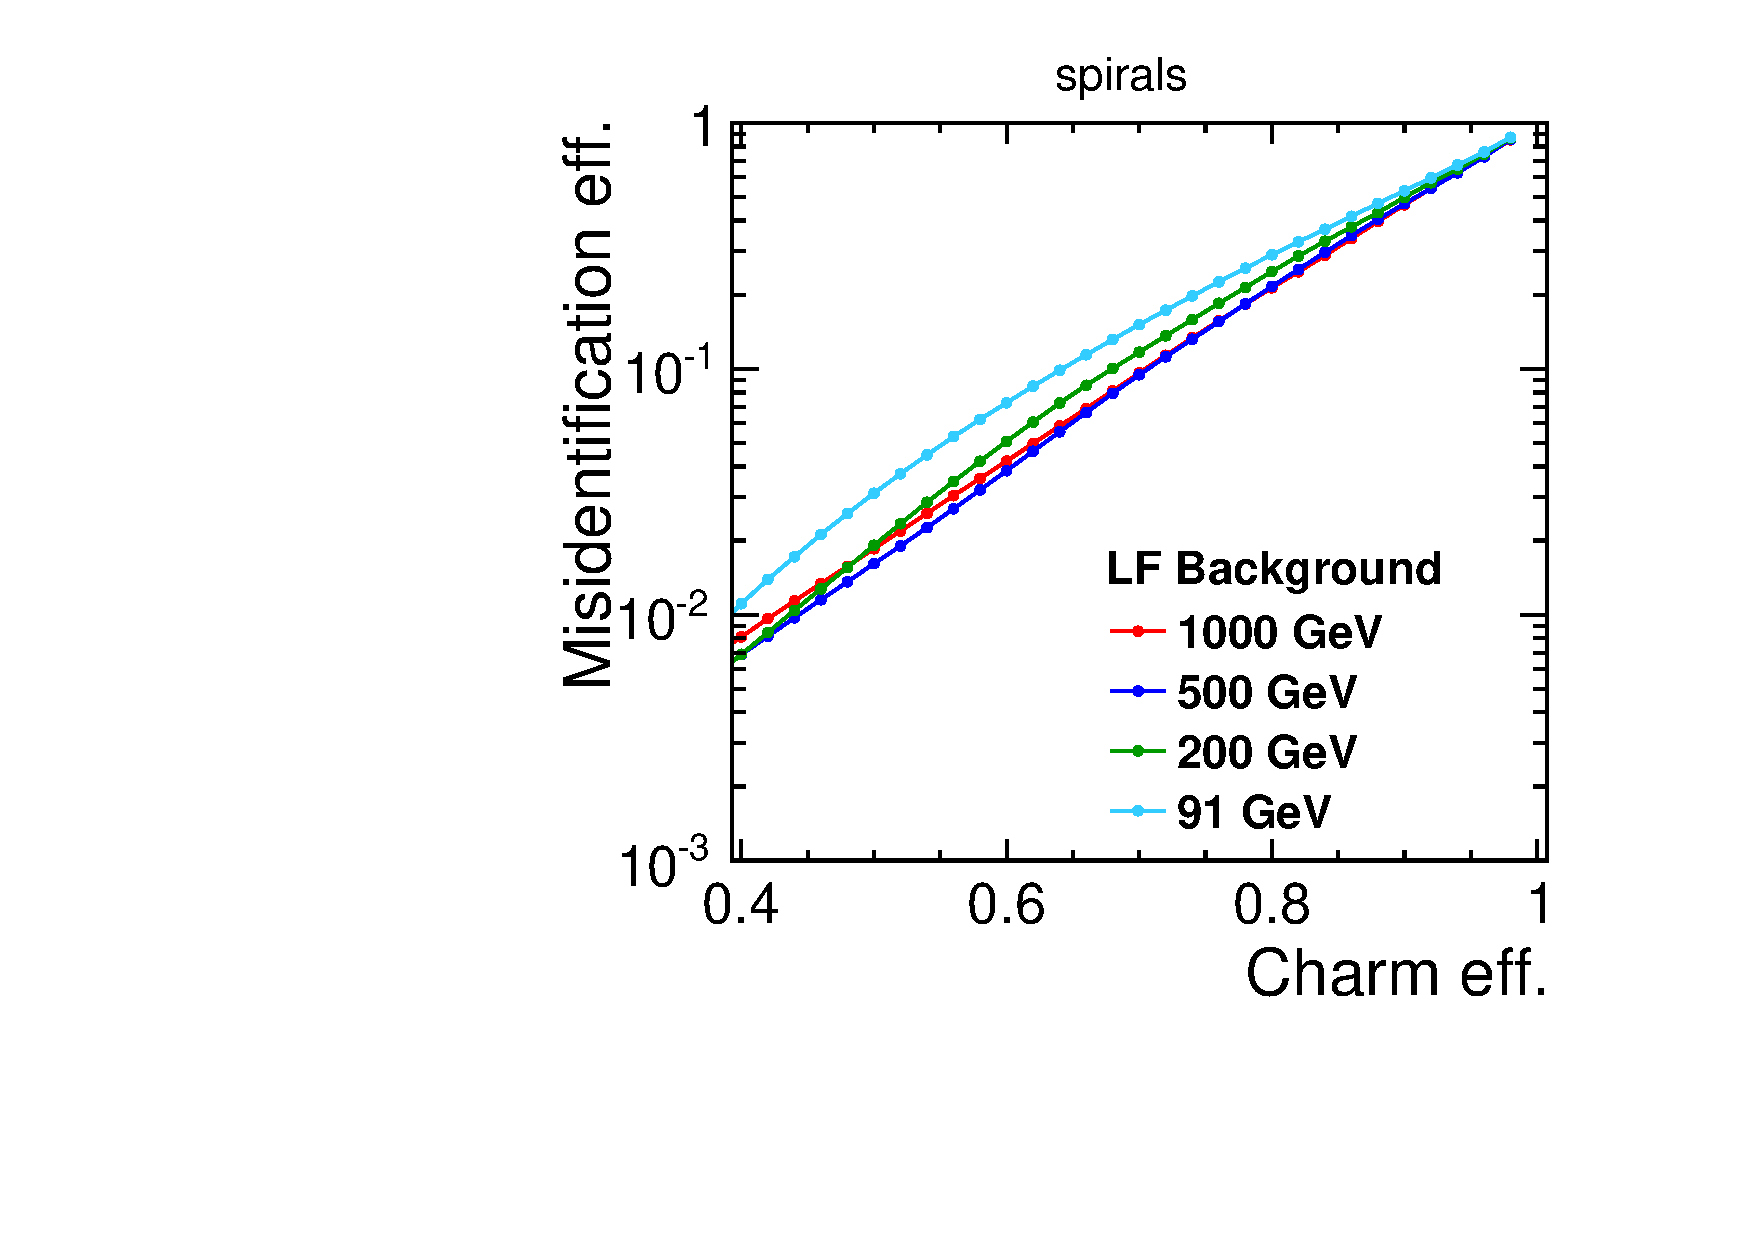
\includegraphics[width=\textwidth]{Figures/ImpactOfGeometries/Global_energies_CLIC_SiD_spirals_Charm_LF_.pdf}
          \caption{}
          \label{}
        \end{subfigure}
        \caption{c-tag efficiencies and fake rates for dijets at a mixture of angles between $10^{\circ}$ and
          $90^{\circ}$ for the \textit{spirals} geometry. (a) shows the fake rate for recognising beauty jets as charm jets and (b) shows the fake rate for recognising light flavour jets as charm jets.}\label{fig:FTEnergyDependenceC}
\end{figure}

\subsection{Jet-angle dependence}
The dependence of the flavour-tagging performance on the jet polar angle is shown in Figures \ref{fig:FTAngleDependenceB} and \ref{fig:FTAngleDependenceC} using the \begin{it}spirals\end{it} geometry for jets in dijet events at $\sqrt{s}=$200~GeV. \\
In the forward region, several factors are causing the sizeable decrease in performance. For low polar angles, some fraction of particles in the jets is not reconstructed along the beam axis. In addition, the vertex detector resolution in
the forward region is worse than in the other parts due to the large
distance between the reconstructed vertex and the sensors (cf. Figures
\ref{fig:spiralRes} and \ref{fig:doubleLayerRes}). In addition, the number of
sensitive layers decreases with decreasing polar angles (cf. Figure~\ref{fig:vertex_nb_layer}). \\
%% In these Figures the errors on the efficiencies are shown to give an
%% idea of the magnitude of the uncertainties. When we compute an efficiency, we select some events among all available events and the uncertainty on the selection is given by Binomial errors. The error is given by: $\sqrt{{e \cdot (1 -e)} \over m}$, where $e$ is the efficiency and $m$ the total number of jets. The errors on the computed efficiencies are very small (around $10^{-4}$). \\
To illustrate the size of the fluctuations due to the finite size of the event samples used, the statistical uncertainties of the obtained misidentification efficiencies are shown by error bars which are negligible.
More results for different jet energies and detector geometries can be found in Appendices~\ref{sec:CDR_jet_angle}, \ref{sec:spirals_jet_angle} and \ref{sec:doubleSpirals_jet_angle}.
\begin{figure}[H]
  \begin{subfigure}[b]{0.5\textwidth}
    \centering
    \begin{tikzpicture}
      \node[anchor=south west,inner sep=0] (image) at (0,0){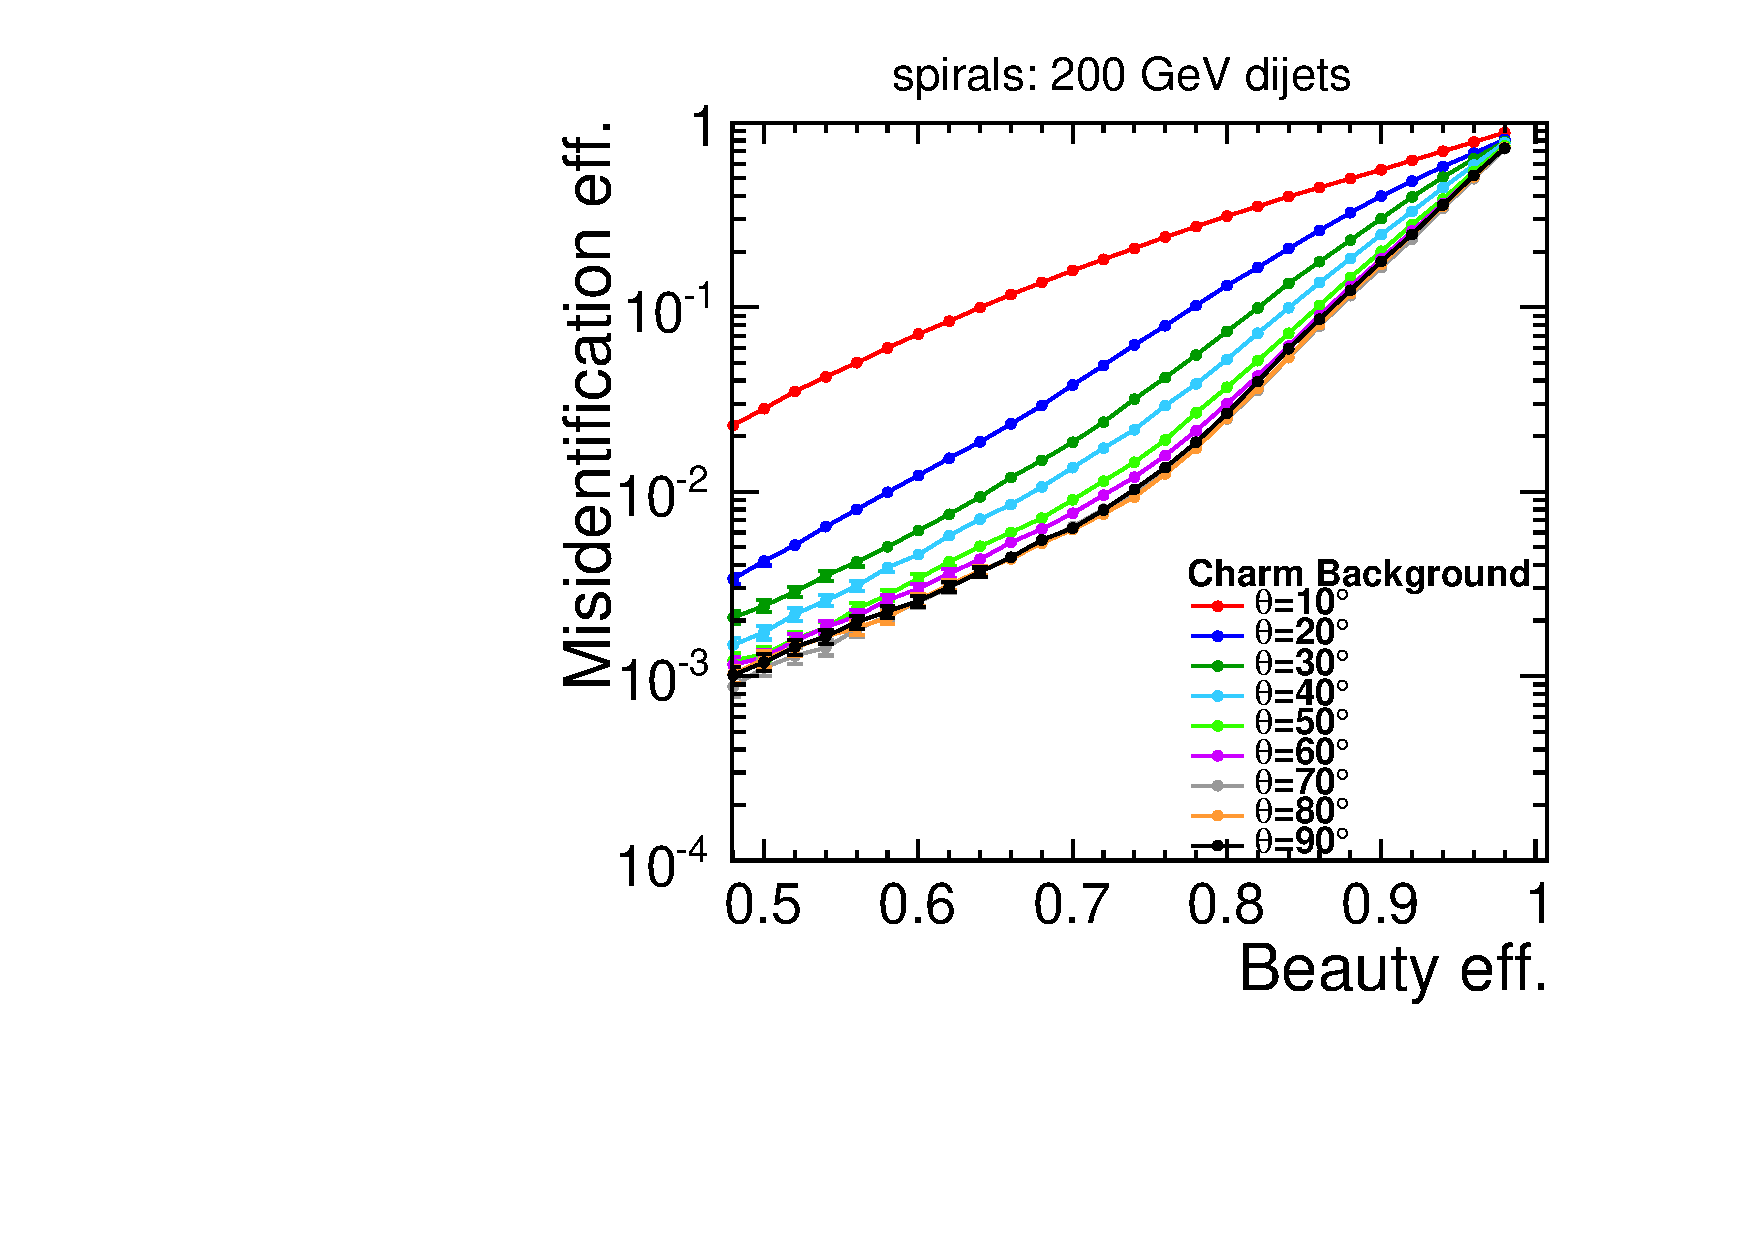
\includegraphics[width=\textwidth]{Figures/ImpactOfGeometries/allAngles_CLIC_SiD_spirals_Beauty_Charm_200.pdf}};
      \draw[white, fill=white] (1.8, 6.3) rectangle (5.7, 7);
    \end{tikzpicture}
    \caption{}
    \label{}
  \end{subfigure}%
  ~ 
  \begin{subfigure}[b]{0.5\textwidth}
    \centering
    \begin{tikzpicture}
      \node[anchor=south west,inner sep=0] (image) at (0,0){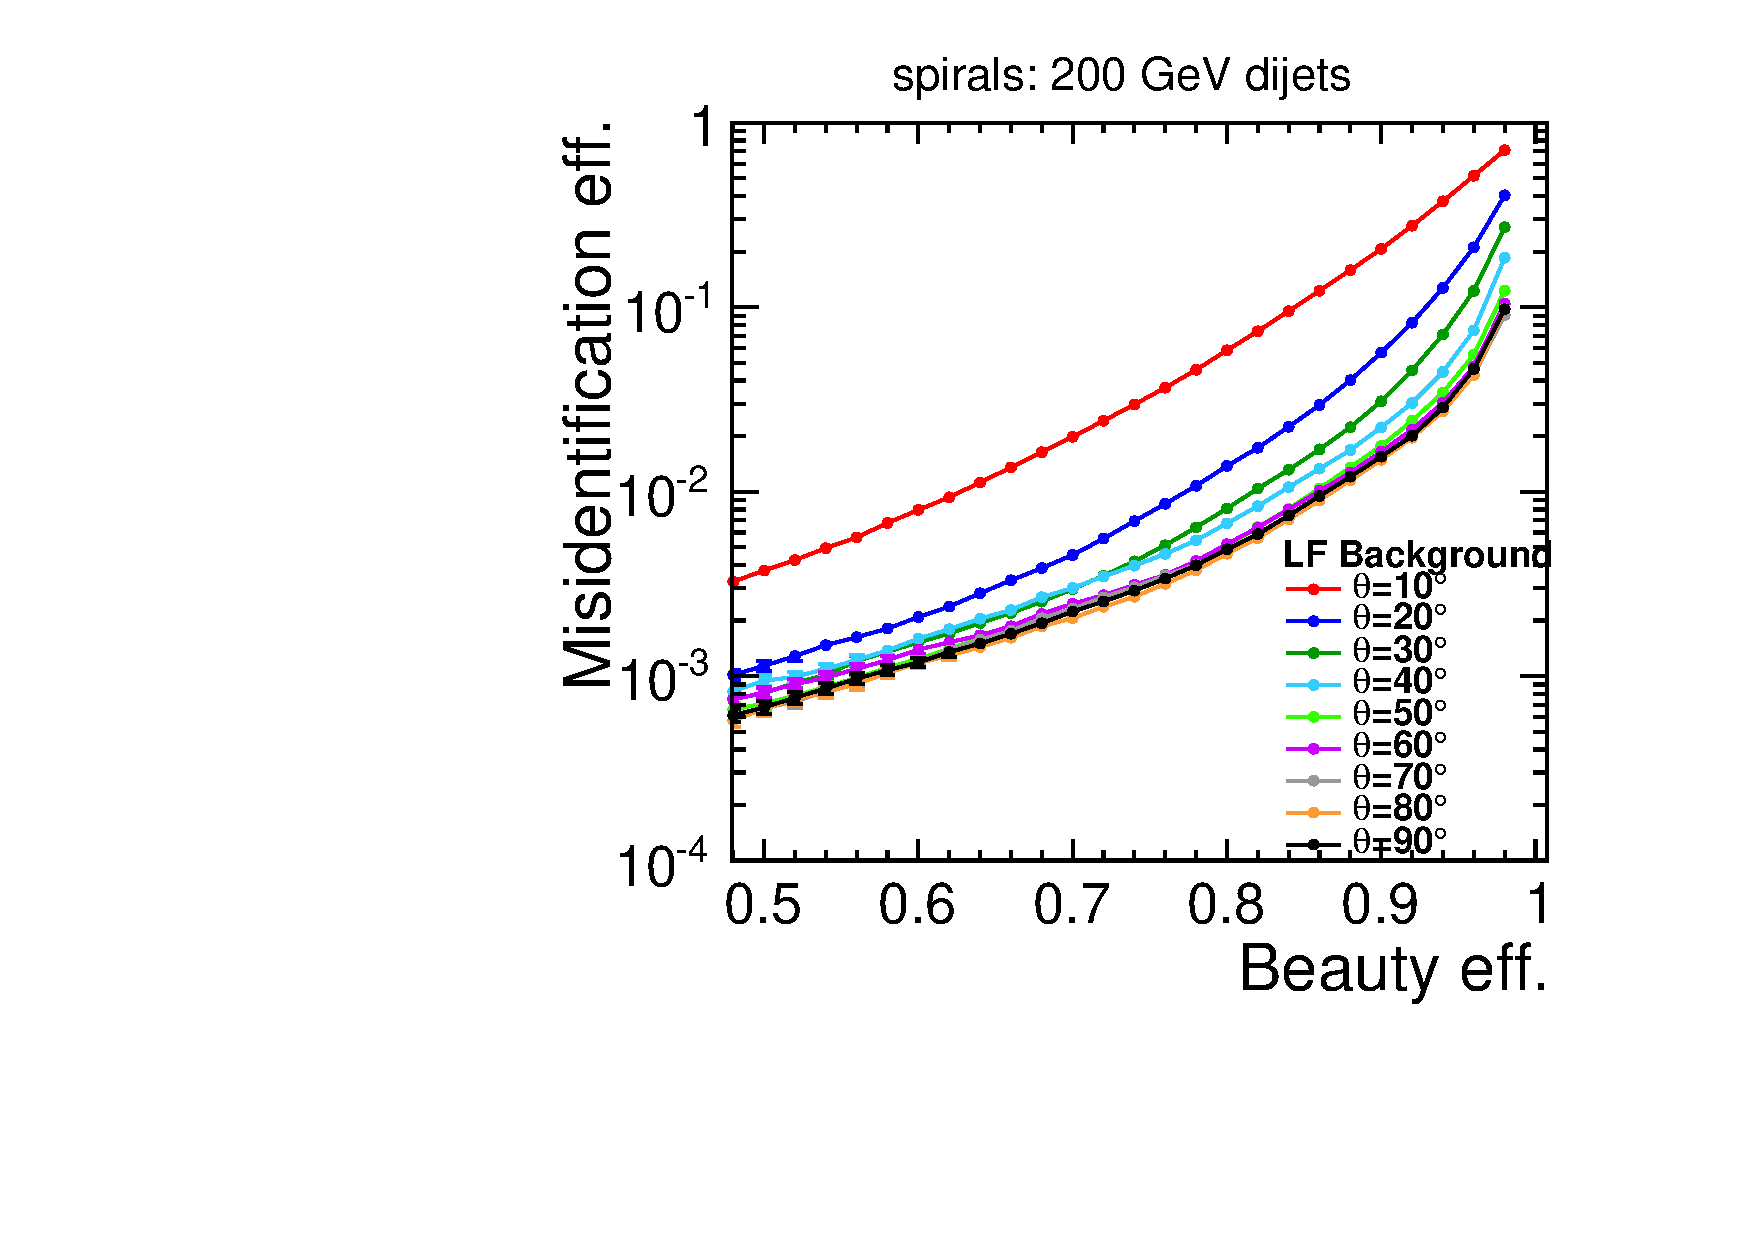
\includegraphics[width=\textwidth]{Figures/ImpactOfGeometries/allAngles_CLIC_SiD_spirals_Beauty_LF_200.pdf}};
      \draw[white, fill=white] (1.8, 6.3) rectangle (5.7, 7);
    \end{tikzpicture}
    \caption{}
    \label{}
  \end{subfigure}
  \caption{b-tag efficiencies for jets in dijet events at $\sqrt{s}=200$~GeV with different polar angles using the \textit{spirals} geometry. (a) shows the fake rate for recognising charm jets as beauty jets and (b) shows the fake rate for recognising light flavour jets as beauty jets.}\label{fig:FTAngleDependenceB}
\end{figure}

\begin{figure}[H]
  \begin{subfigure}[b]{0.5\textwidth}
    \centering
    \begin{tikzpicture}
      \node[anchor=south west,inner sep=0] (image) at (0,0){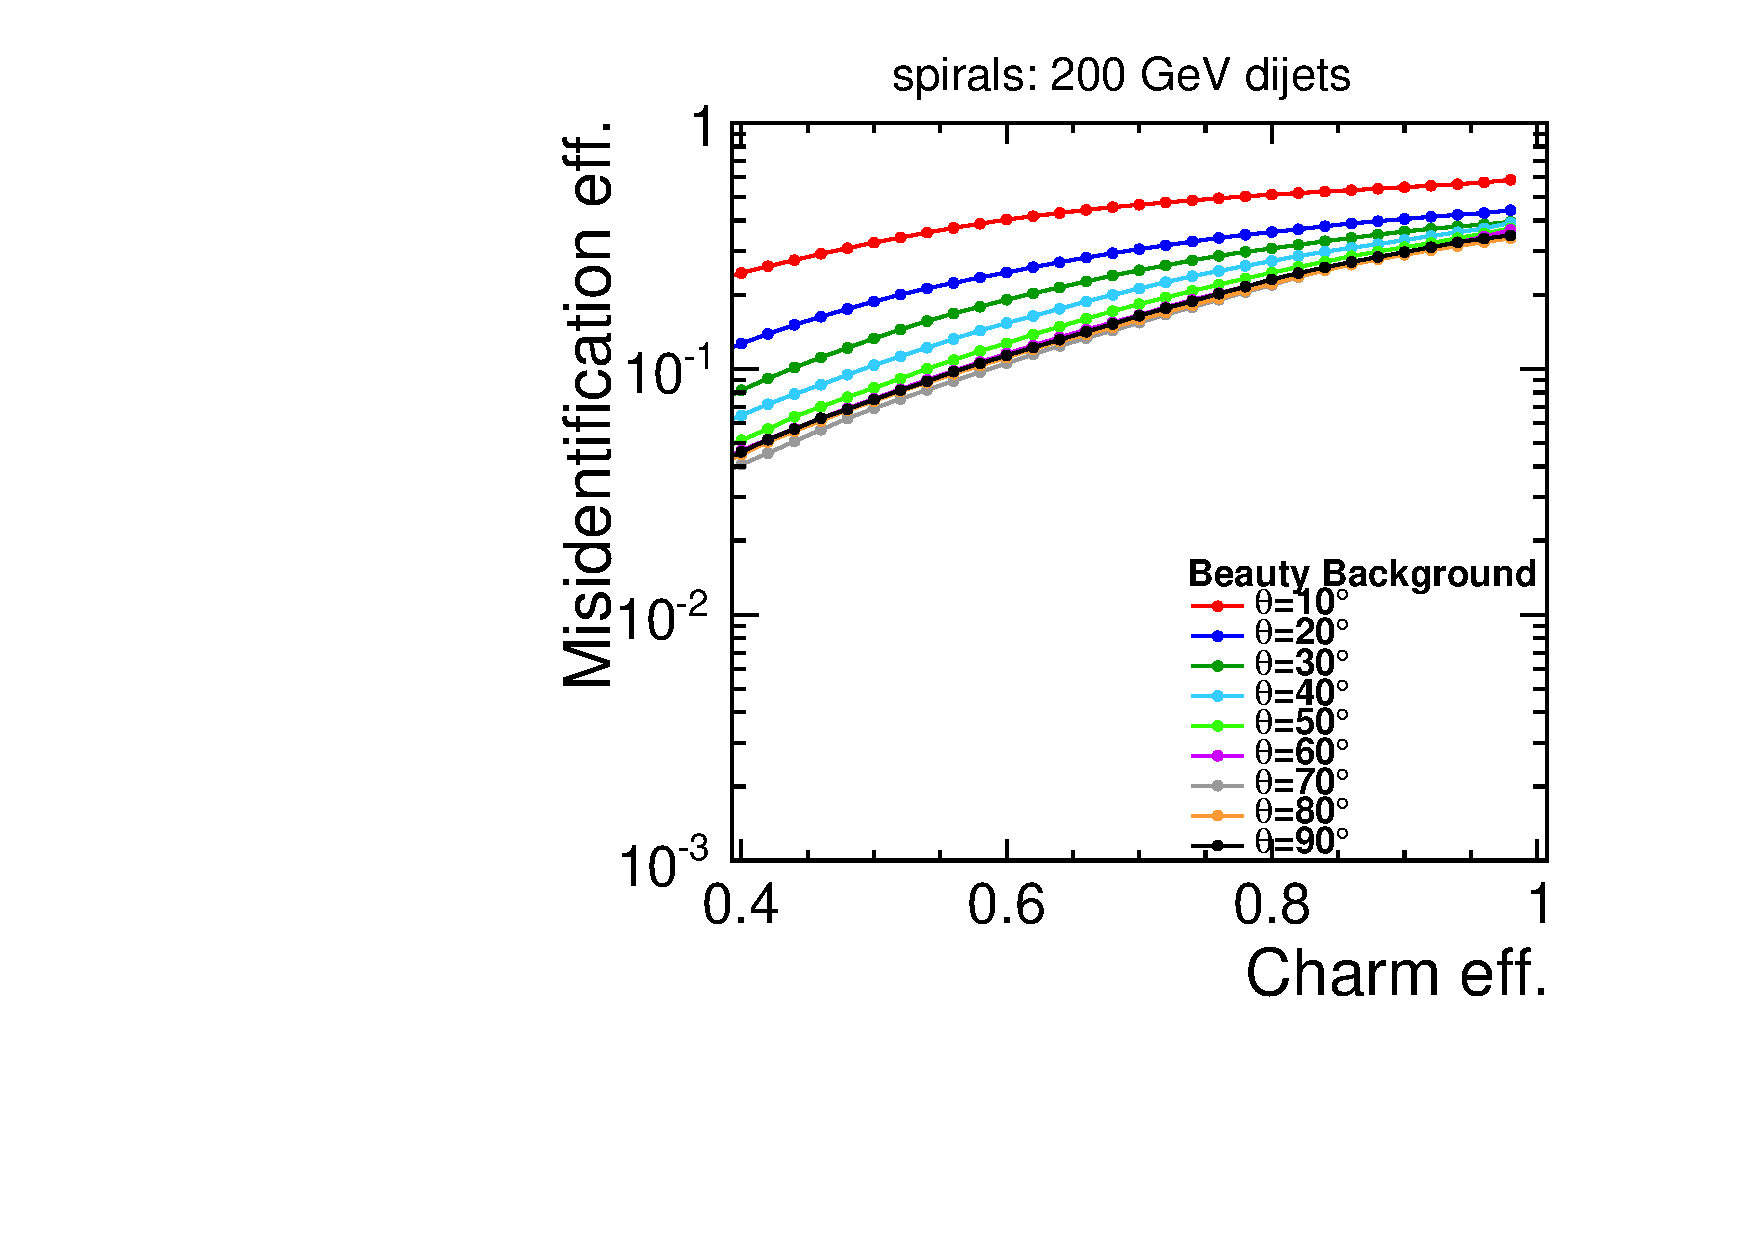
\includegraphics[width=\textwidth]{Figures/ImpactOfGeometries/allAngles_CLIC_SiD_spirals_Charm_Beauty_200.pdf}};
      \draw[white, fill=white] (1.8, 6.3) rectangle (5.7, 7);
    \end{tikzpicture}
    \caption{}
    \label{}
  \end{subfigure}%
  ~ 
  \begin{subfigure}[b]{0.5\textwidth}
    \centering
    \begin{tikzpicture}
      \node[anchor=south west,inner sep=0] (image) at (0,0){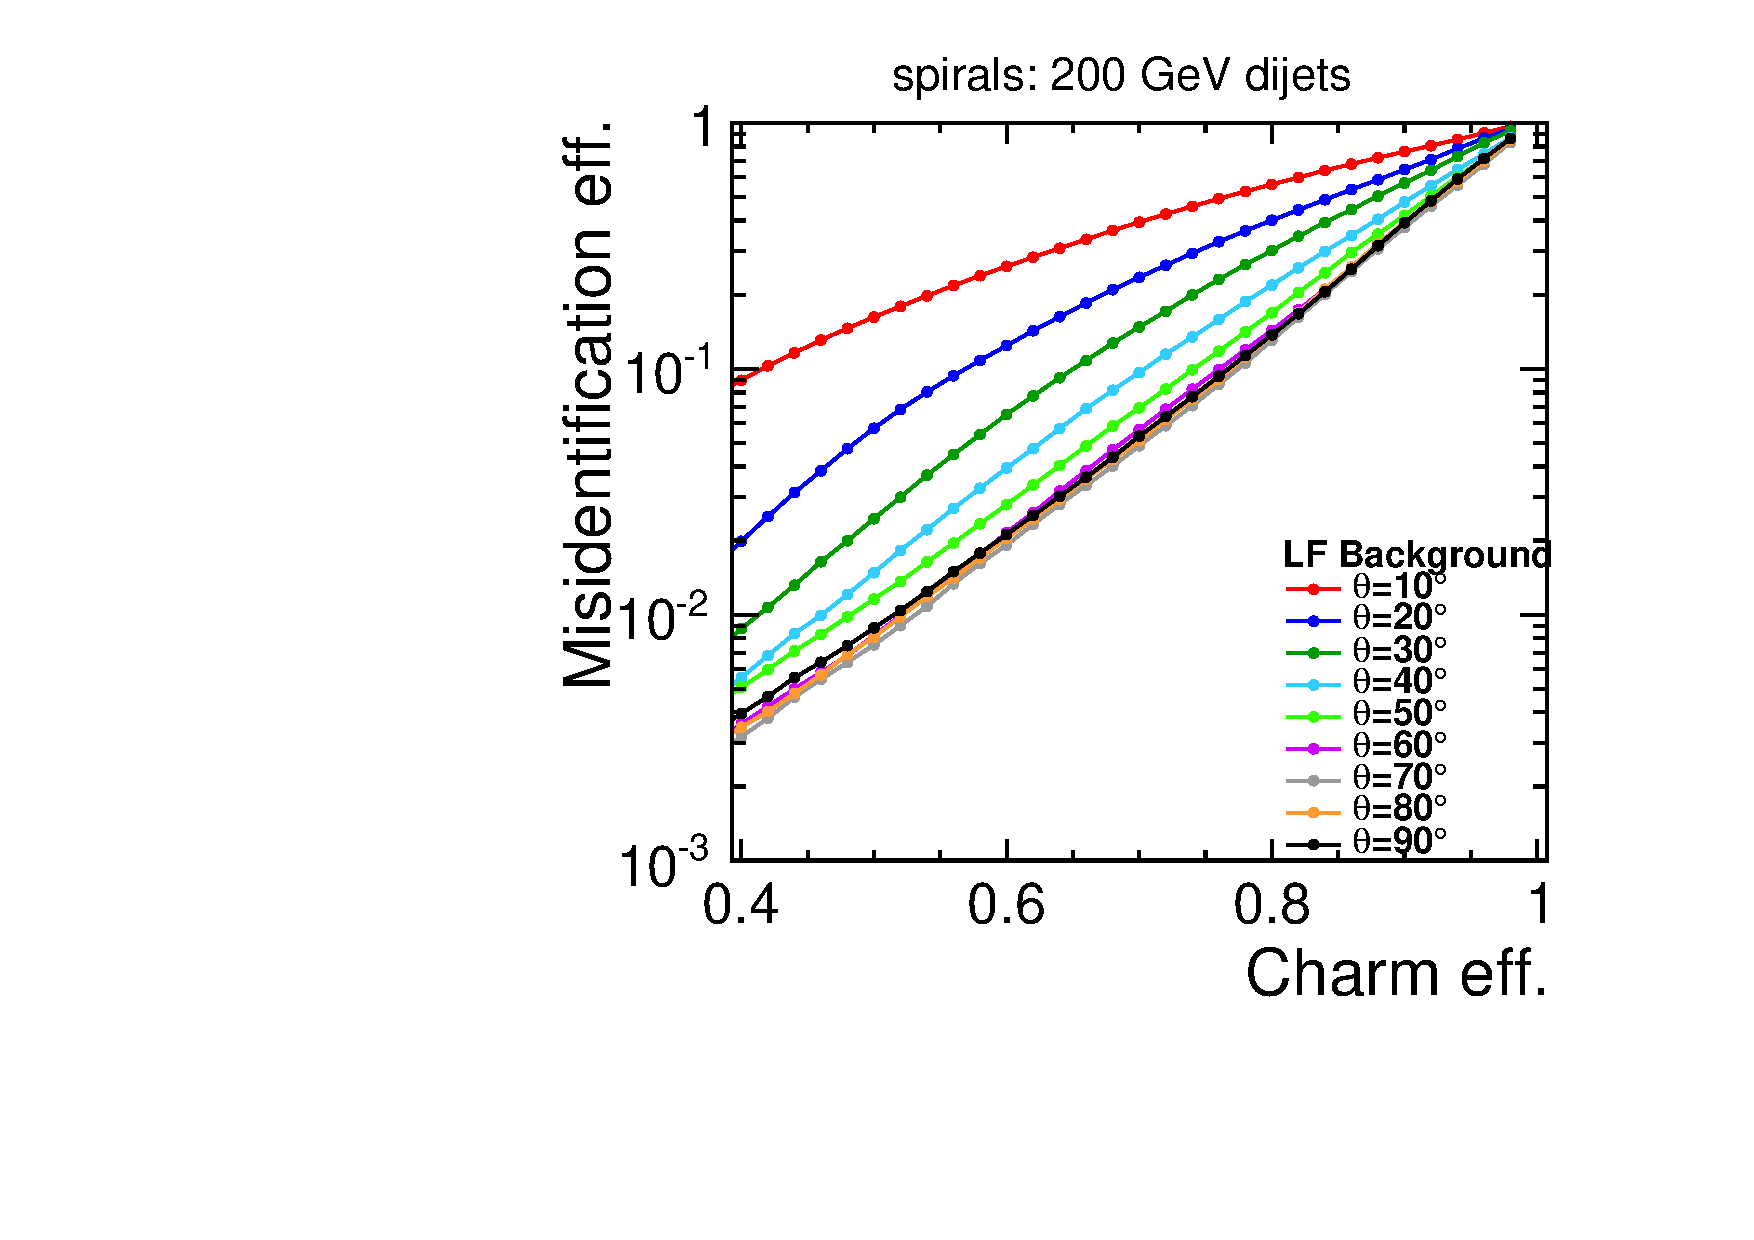
\includegraphics[width=\textwidth]{Figures/ImpactOfGeometries/allAngles_CLIC_SiD_spirals_Charm_LF_200.pdf}};
      \draw[white, fill=white] (1.8, 6.3) rectangle (5.7, 7);
    \end{tikzpicture}
    \caption{}
    \label{}
  \end{subfigure}
  \caption{c-tag efficiencies for jets in dijet events at $\sqrt{s}=200$~GeV with different polar angles using the \textit{spirals} geometry. (a) shows the fake rate for recognising beauty jets as charm jets and (b) shows the fake rate for recognising light flavour jets as charm jets.}\label{fig:FTAngleDependenceC}
\end{figure}

\subsection{Comparison of different layouts}

In the following sections, the different geometries are compared based on their flavour-tagging performance. First, the spiral configuration is compared to the disks in the endcap regions. Then, the double-layered sensors are compared to the single-layered sensors. Finally, the \textit{double\_spirals} geometry is compared to the CDR geometry.


%% \begin{figure}[H]
%%   \centering
%%   \includegraphics[scale=0.4]{Figures/}
%%   \caption{}
%%   \label{}
%% \end{figure}

%----------------------------------------------------------------------
\subsubsection{\emph{spirals} and CDR}\label{sec:spirals_CDR}

In order to compare two geometries in terms of flavour-tagging performance, the ratio between the misidentification probabilities is computed. \\
Figures \ref{fig:spirals_disks_beauty} and \ref{fig:spirals_disks_charm} compare the CDR and the \textit{spirals} geometry using jets in dijet events at $\sqrt{s}=200$~GeV with polar angles of $\theta=10^\circ, 20^\circ, 30^\circ$ and $40^\circ$. If the ratio between the misidentification probabilities is smaller than one, then the \textit{spirals} geometry has a better flavour-tagging performance than the CDR geometry. Otherwise, the CDR geometry has a better performance.
In general, the two geometries have a similar performance. However, the b-tagging performance is up to $20\%$ worse using the \textit{spirals} geometry for jets at $\theta=40^{\circ}$. At this angle, there is the transition between the vertex endcaps and the barrel region. With the spiral configuration, the number of sensitive layers becomes dependent on the azimuthal angle $\phi$. Less layers can be hit for the spiral configurations in certain ranges in the azimuthal angle $\phi$ compared to the CDR geometry where the number of layers in the endcap regions does not depend on $\phi$ (cf. Figure~\ref{fig:nbLayers_theta_phi}). The track-finding algorithm requires a minimum number of layers hit in the vertex detector. This requirement is not dependent on the $\phi$ direction of the track. Hence with the current software implementation, it is more likely that tracks in a certain $\phi$ region are missed compared to the CDR geometry. This can be improved in future tracking code with using a $\phi$-dependent optimisation of the track finding strategy. \\
More results for different jet energies can be found in Appendix~\ref{sec:appendix_spirals_vs_CDR}.

\begin{figure}[H]
  \begin{subfigure}[b]{0.5\textwidth}
    \centering
    \begin{tikzpicture}
      \node[anchor=south west,inner sep=0] (image) at (0,0){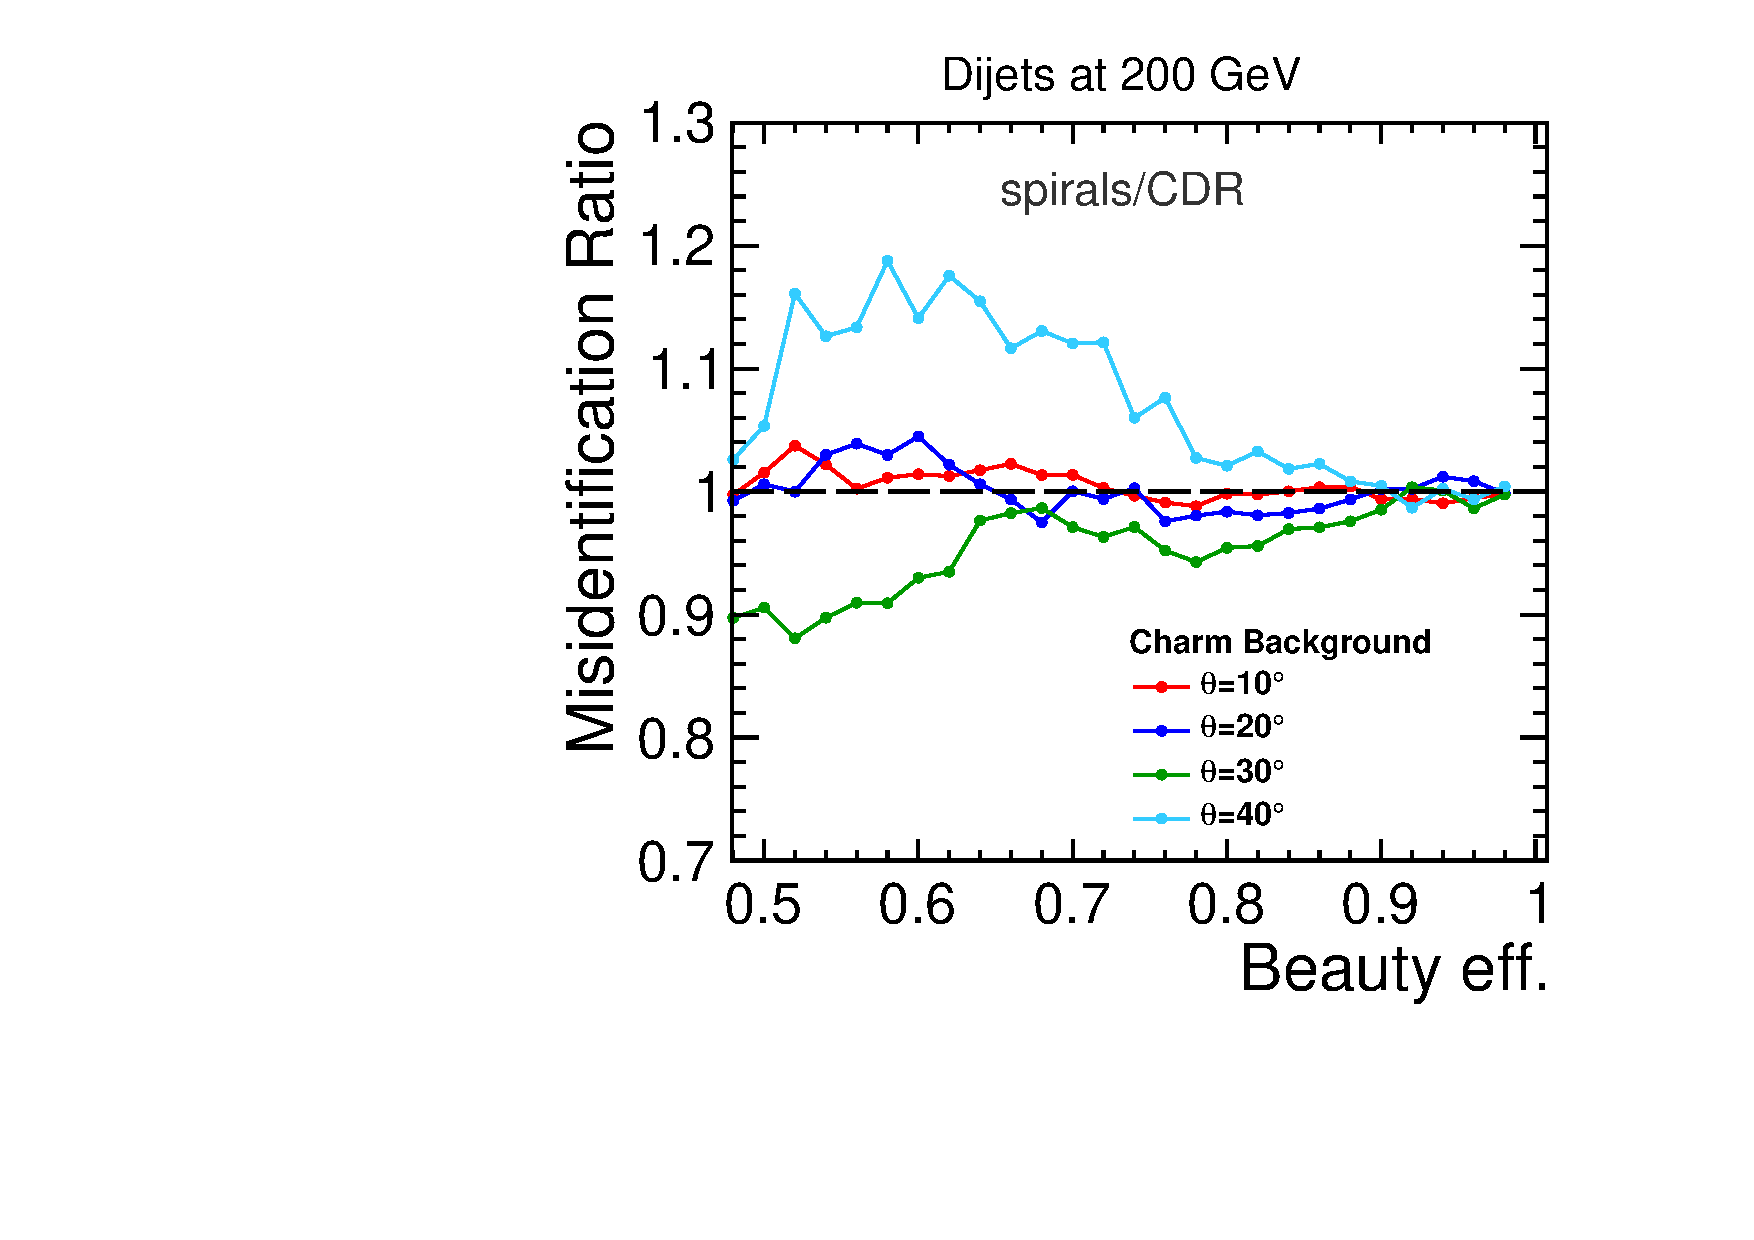
\includegraphics[width=\textwidth]{Figures/ImpactOfGeometries/200GeV_Ratio_allAngles_spirals_CDR_B_C.pdf}};
      \draw[white, fill=white] (1.8, 6.3) rectangle (5.7, 7);
    \end{tikzpicture}
    \caption{}
    \label{fig:200GeV_Ratio_allAngles_spirals_CDR_B_C.pdf}
  \end{subfigure}%
  ~ 
  \begin{subfigure}[b]{0.5\textwidth}
    \centering
    \begin{tikzpicture}
      \node[anchor=south west,inner sep=0] (image) at (0,0){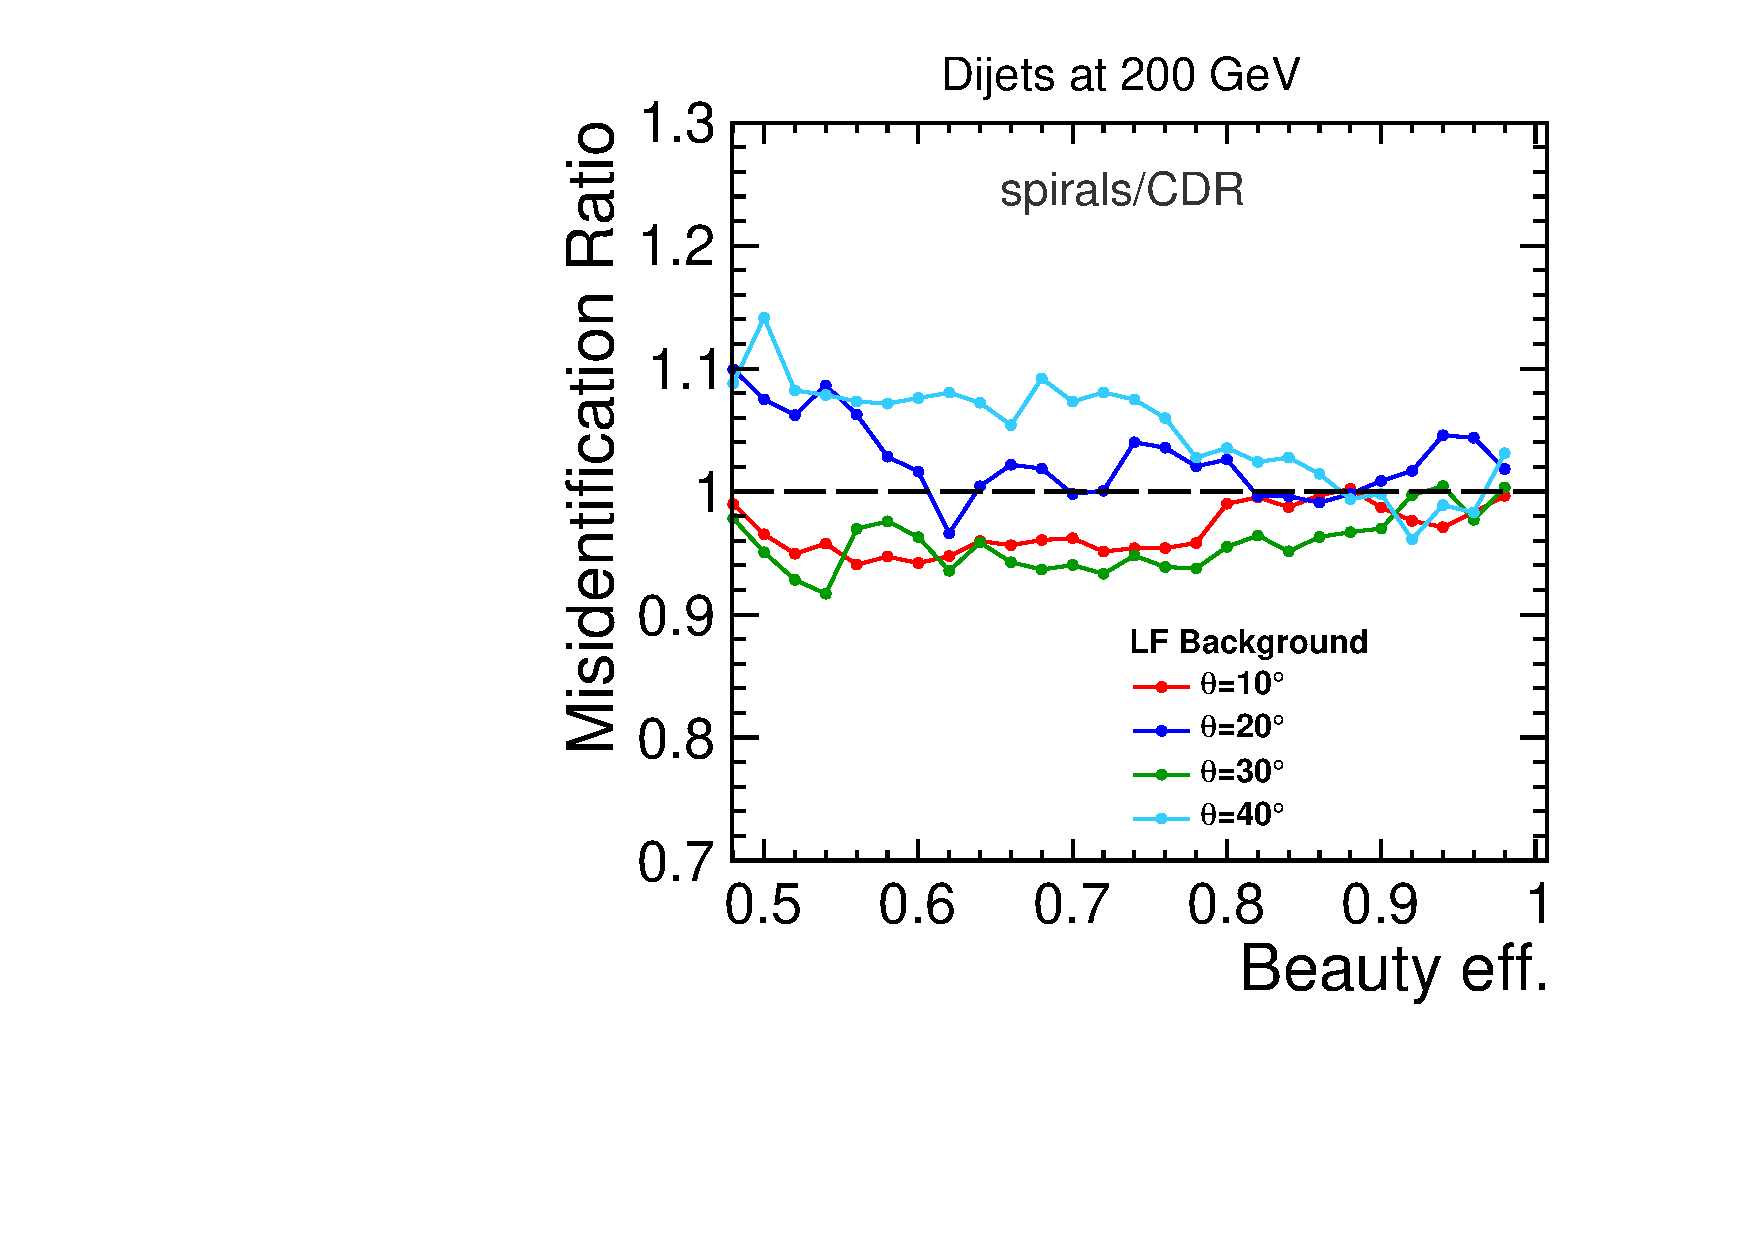
\includegraphics[width=\textwidth]{Figures/ImpactOfGeometries/200GeV_Ratio_allAngles_spirals_CDR_B_LF.pdf}};
      \draw[white, fill=white] (1.8, 6.3) rectangle (5.7, 7);
    \end{tikzpicture}
    \caption{}
    \label{fig:200GeV_Ratio_allAngles_spirals_CDR_B_LF.pdf}
  \end{subfigure}
  \caption{The ratios between the misidentification probabilities for the \textit{spirals} and the CDR geometries as a function of the b-tag efficiency considering the charm (a) and the light flavour (b) backgrounds based on jets in dijet events at $\sqrt{s}=200$~GeV.}\label{fig:spirals_disks_beauty}
\end{figure}

\begin{figure}[H]
  \begin{subfigure}[b]{0.5\textwidth}
    \centering
    \begin{tikzpicture}
      \node[anchor=south west,inner sep=0] (image) at (0,0){\includegraphics[width=\textwidth]{Figures/ImpactOfGeometries/200GeV_Ratio_allAngles_spirals_CDR_C_B.pdf}};
      \draw[white, fill=white] (1.8, 6.3) rectangle (5.7, 7);
    \end{tikzpicture}
    \caption{}
    \label{ref:200GeV_Ratio_allAngles_spirals_CDR_C_B.pdf}
  \end{subfigure}%
  ~ 
  \begin{subfigure}[b]{0.5\textwidth}
    \centering
    \begin{tikzpicture}
      \node[anchor=south west,inner sep=0] (image) at (0,0){\includegraphics[width=\textwidth]{Figures/ImpactOfGeometries/200GeV_Ratio_allAngles_spirals_CDR_C_LF.pdf}};
      \draw[white, fill=white] (1.8, 6.3) rectangle (5.7, 7);
    \end{tikzpicture}
    \caption{}
    \label{ref:200GeV_Ratio_allAngles_spirals_CDR_C_LF.pdf}
  \end{subfigure}
  \caption{The ratios between the misidentification probabilities for the \textit{spirals} and the CDR geometries as a function of the c-tag efficiency considering the beauty (a) and the light flavour (b) backgrounds based on jets in dijet events at $\sqrt{s}=200$~GeV.}\label{fig:spirals_disks_charm}
\end{figure}


%----------------------------------------------------------------------
\subsubsection{\emph{double\_spirals} and \emph{spirals}}

The \begin{it}double\_spirals\end{it} and the \textit{spirals} geometries are compared using dijet events with a mixture of polar angles between $10^{\circ}$ and $90^{\circ}$. For each jet flavour, 720000 events are included (for each $\theta$ value, the same number of events is used). Having large number of events allows to reduce the statistical fluctuations.\\
The comparison between the two geometries is shown in Figures \ref{fig:globalComparison_double_spirals_1000}, \ref{fig:globalComparison_double_spirals_500}, \ref{fig:globalComparison_double_spirals_200} and \ref{fig:globalComparison_double_spirals_91}. The performances of these two geometries are similar.\\ 
For jets in dijet events at $\sqrt{s}=$1000~GeV, the \textit{double\_spirals} geometry shows a better performance for beauty and charm tagging. For jets in dijet events at $\sqrt{s}=$500~GeV and $\sqrt{s}=$200~GeV, the ratio between the misidentification probabilities varies between $\pm 10\%$. For jets in dijet events at $\sqrt{s}=$91~GeV, the c-tag performance shows better results for light-flavour rejection with the \textit{double\_spirals} geometry. This effect might be explained by the fact that double-sided modules provide two measurements which are close to the interaction point and improve the track reconstruction. In some cases, it is possible that the B hadron decays after the first layer in the vertex barrel. In the CDR and the \textit{spirals} geometry, one measurement layer is lost. With the \textit{double\_spirals} configuration, two measurement layers are lost. But in total, the number of hits is identical if the decay of the B hadrons occurs after the first layer for the three geometries.\\
More results for different jet energies and angles can be found in Appendix~\ref{sec:appendix_doubleSpirals_vs_spirals}.

\begin{figure}[H]
  \begin{subfigure}[b]{0.5\textwidth}
    \centering
    \begin{tikzpicture}
      \node[anchor=south west,inner sep=0] (image) at (0,0){\includegraphics[width=\textwidth]{Figures/ImpactOfGeometries/general_1000_Beauty.pdf}};
      \draw[white, fill=white] (1.8, 9.95) rectangle (5.5, 10.6);
    \end{tikzpicture}
    \caption{}
    \label{}
  \end{subfigure}%
  ~ 
  \begin{subfigure}[b]{0.5\textwidth}
    \centering
    \begin{tikzpicture}
      \node[anchor=south west,inner sep=0] (image) at (0,0){\includegraphics[width=\textwidth]{Figures/ImpactOfGeometries/general_1000_Charm.pdf}};
      \draw[white, fill=white] (1.8, 9.95) rectangle (5.5, 10.6);
    \end{tikzpicture}
    \caption{}
    \label{}
  \end{subfigure}
  \caption{Global comparison between the \textit{double\_spirals} and the
    \textit{spirals} geometries based on beauty tagging (a) and charm
    tagging (b) for jets in dijet events at $\sqrt{s}=$1000~GeV with a
    mixture of polar angles between $10^{\circ}$ and $90^{\circ}$. On the y-axis, the misidentification probability and the ratio between the misidentification probabilities for the two geometries are given.}\label{fig:globalComparison_double_spirals_1000}
\end{figure}

\begin{figure}[H]
  \begin{subfigure}[b]{0.5\textwidth}
    \centering
    \begin{tikzpicture}
      \node[anchor=south west,inner sep=0] (image) at (0,0){\includegraphics[width=\textwidth]{Figures/ImpactOfGeometries/general_500_Beauty.pdf}};
      \draw[white, fill=white] (1.8, 9.95) rectangle (5.5, 10.6);
    \end{tikzpicture}
    \caption{}
    \label{}
  \end{subfigure}%
  ~ 
  \begin{subfigure}[b]{0.5\textwidth}
    \centering
        \begin{tikzpicture}
      \node[anchor=south west,inner sep=0] (image) at (0,0){\includegraphics[width=\textwidth]{Figures/ImpactOfGeometries/general_500_Charm.pdf}};
      \draw[white, fill=white] (1.8, 9.95) rectangle (5.5, 10.6);
        \end{tikzpicture}
        \caption{}
        \label{}
  \end{subfigure}
  \caption{Global comparison between the \textit{double\_spirals} and the
    \textit{spirals} geometries based on beauty tagging (a) and charm
    tagging (b) for jets in dijet events at $\sqrt{s}=$500~GeV with a mixture of polar
    angles between $10^{\circ}$ and $90^{\circ}$. On the y-axis, the misidentification probability and the ratio between the misidentification probabilities for the two geometries are given.}\label{fig:globalComparison_double_spirals_500}
\end{figure}

\begin{figure}[H]
  \begin{subfigure}[b]{0.5\textwidth}
    \centering
    \begin{tikzpicture}
      \node[anchor=south west,inner sep=0] (image) at (0,0){\includegraphics[width=\textwidth]{Figures/ImpactOfGeometries/general_200_Beauty.pdf}};
      \draw[white, fill=white] (1.8, 9.95) rectangle (5.5, 10.6);
    \end{tikzpicture}
    \caption{}
    \label{}
  \end{subfigure}%
  ~ 
  \begin{subfigure}[b]{0.5\textwidth}
    \centering
    \begin{tikzpicture}
      \node[anchor=south west,inner sep=0] (image) at (0,0){\includegraphics[width=\textwidth]{Figures/ImpactOfGeometries/general_200_Charm.pdf}};
      \draw[white, fill=white] (1.8, 9.95) rectangle (5.5, 10.6);
    \end{tikzpicture}
    \caption{}
    \label{}
  \end{subfigure}
  \caption{Global comparison between the \textit{double\_spirals} and the \textit{spirals} geometries based on beauty tagging (a) and charm
    tagging (b) for jets in dijet events at $\sqrt{s}=$200~GeV with a mixture of polar
    angles between $10^{\circ}$ and $90^{\circ}$. On the y-axis, the misidentification probability and the ratio between the misidentification probabilities for the two geometries are given.}\label{fig:globalComparison_double_spirals_200}
\end{figure}

\begin{figure}[H]
  \begin{subfigure}[b]{0.5\textwidth}
    \centering
    \begin{tikzpicture}
      \node[anchor=south west,inner sep=0] (image) at (0,0){\includegraphics[width=\textwidth]{Figures/ImpactOfGeometries/general_91_Beauty.pdf}};
      \draw[white, fill=white] (1.8, 9.95) rectangle (5.5, 10.6);
    \end{tikzpicture}
    \caption{}
    \label{}
  \end{subfigure}%
  ~ 
  \begin{subfigure}[b]{0.5\textwidth}
    \centering
    \begin{tikzpicture}
      \node[anchor=south west,inner sep=0] (image) at (0,0){\includegraphics[width=\textwidth]{Figures/ImpactOfGeometries/general_91_Charm.pdf}};
      \draw[white, fill=white] (1.8, 9.95) rectangle (5.5, 10.6);
    \end{tikzpicture}
    \caption{}
    \label{}
  \end{subfigure}
  \caption{Global comparison between the \textit{double\_spirals} and the
    \textit{spirals} geometries based on beauty tagging (a) and charm
    tagging (b) for jets in dijet events at $\sqrt{s}=$91~GeV with a
    mixture of polar angles between $10^{\circ}$ and $90^{\circ}$. On the y-axis, the misidentification probability and the ratio between the misidentification probabilities for the two geometries are given.}\label{fig:globalComparison_double_spirals_91}
\end{figure}


%----------------------------------------------------------------------
\subsubsection{\emph{double\_spirals} and CDR}
The comparison between the \textit{double\_spirals} and the CDR geometries is given in Figures \ref{fig:double_disks_beauty} and \ref{fig:double_disks_charm}. \\
In general, the performance of the two geometries is very similar except for dijet events at $\theta=40^\circ$ where the b-tagging performance for the \textit{double\_spirals} geometry decreases by up to 30\% (the same effect is also observed when comparing the \textit{spirals} and the CDR geometries in Section \ref{sec:spirals_CDR}). This polar angle falls in the transition region between the vertex endcaps and barrel. The same effect is discussed in Section~\ref{sec:spirals_CDR}. \\
More results for different jet energies can be found in Appendix~\ref{sec:appendix_doubleSpirals_vs_CDR}.

\begin{figure}[H]
  \begin{subfigure}[b]{0.5\textwidth}
    \centering
    \begin{tikzpicture}
      \node[anchor=south west,inner sep=0] (image) at (0,0){\includegraphics[width=\textwidth]{Figures/ImpactOfGeometries/200GeV_Ratio_allAngles_doubleSpirals_CDR_B_C.pdf}};
      \draw[white, fill=white] (1.8, 6.3) rectangle (5.7, 7);
    \end{tikzpicture}
    \caption{}
    \label{}
  \end{subfigure}%
  ~ 
  \begin{subfigure}[b]{0.5\textwidth}
    \centering
    \begin{tikzpicture}
      \node[anchor=south west,inner sep=0] (image) at (0,0){\includegraphics[width=\textwidth]{Figures/ImpactOfGeometries/200GeV_Ratio_allAngles_doubleSpirals_CDR_B_LF.pdf}};
      \draw[white, fill=white] (1.8, 6.3) rectangle (5.7, 7);
    \end{tikzpicture}
    \caption{}
    \label{}
  \end{subfigure}
  \caption{The ratios between the misidentification
    probabilities for the \textit{double\_spirals} and the CDR geometries
    as function of the b-tag efficiency considering the charm
    (a) and the light flavour (b) backgrounds based on jets in dijet events at $\sqrt{s}=200$~GeV.}\label{fig:double_disks_beauty}
\end{figure}

\begin{figure}[H]
  \begin{subfigure}[b]{0.5\textwidth}
    \centering
    \begin{tikzpicture}
      \node[anchor=south west,inner sep=0] (image) at (0,0){\includegraphics[width=\textwidth]{Figures/ImpactOfGeometries/200GeV_Ratio_allAngles_doubleSpirals_CDR_C_B.pdf}};
      \draw[white, fill=white] (1.8, 6.3) rectangle (5.7, 7);
    \end{tikzpicture}
    \caption{}
    \label{}
  \end{subfigure}%
  ~ 
  \begin{subfigure}[b]{0.5\textwidth}
    \centering
    \begin{tikzpicture}
      \node[anchor=south west,inner sep=0] (image) at (0,0){\includegraphics[width=\textwidth]{Figures/ImpactOfGeometries/200GeV_Ratio_allAngles_doubleSpirals_CDR_C_LF.pdf}};
      \draw[white, fill=white] (1.8, 6.3) rectangle (5.7, 7);
    \end{tikzpicture}
    \caption{}
    \label{}
  \end{subfigure}
  \caption{The ratios between the misidentification
    probabilities for the \textit{double\_spirals} and the CDR geometries
    as function of the c-tag efficiency considering the beauty
    (a) and the light flavour (b) backgrounds based on jets in dijet events at $\sqrt{s}=200$~GeV.}\label{fig:double_disks_charm}
\end{figure}



\subsection{Impact of the material budget}\label{sec:impactOfMaterialBudget}

The {\it double\_spirals\_v2} geometry is a more realistic version of
the {\it double\_spirals} geometry, taking into account the material
used for the mechanical support of the sensors and also the material
used for the cables. The material budget per double layer is 0.4\%~X$_{0}$.
The flavour-tagging performance of this geometry is given in Figure~\ref{fig:heavy_200} and compared to the \textit{double\_spirals} layout. Dijet events
with a mixture of polar angles between $10^{\circ}$ and $90^{\circ}$ are used for the flavour tagging.\\
By increasing the material in the vertex detector, the fake rate increases by approximately 5-35\% depending on the
required signal efficiency and background type.


\begin{figure}[H]
  \begin{subfigure}[b]{0.5\textwidth}
    \centering
    \begin{tikzpicture}
      \node[anchor=south west,inner sep=0] (image) at (0,0){\includegraphics[width=\textwidth]{Figures/ImpactOfGeometries/heavy_general_200_Beauty.pdf}};
      \draw[white, fill=white] (1.8, 9.95) rectangle (5.5, 10.6);
    \end{tikzpicture}
    \caption{}
    \label{}
  \end{subfigure}%
  ~ 
  \begin{subfigure}[b]{0.5\textwidth}
    \centering
    \begin{tikzpicture}
      \node[anchor=south west,inner sep=0] (image) at (0,0){\includegraphics[width=\textwidth]{Figures/ImpactOfGeometries/heavy_general_200_Charm.pdf}};
      \draw[white, fill=white] (1.8, 9.95) rectangle (5.5, 10.6);
    \end{tikzpicture}
    \caption{}
    \label{}
  \end{subfigure}
  \caption{Global comparison between the \textit{double\_spirals\_v2} and
    the \textit{double\_spirals} geometries based on beauty tagging (a)
    and charm tagging (b) for jets in dijet events at $\sqrt{s}=$200~GeV with a
    mixture of polar angles between $10^{\circ}$ and
    $90^{\circ}$. On the y-axis, the misidentification probability
    and the ratio between the misidentification probabilities for
    the two geometries are given.}\label{fig:heavy_200}
\end{figure}

%----------------------------------------------------------------------


%
%%%%%%%%%\section{The impact of the material budget}\label{sec:impactOfMaterialBudget}

The double\_spirals\_v2 geometry is a more realistic version of the double\_spirals geometry which takes into account the material used for the mechanical support of the sensors and also the material used for the powering of the chip. The material budget per double layer is 0.4\%~X$_{0}$.
The flavor-tagging performance of this geometry is given in Figure \ref{fig:heavy_200} and compared to the double\_spirals. Dijet events with a mixture of angles are used for the flavour tagging.\\
Indeed, by increasing the material in the vertex detector, the performance of the flavour tagging decreases by up to 40\%.


\begin{figure}[H]
        \begin{subfigure}[b]{0.5\textwidth}
          \centering
          \includegraphics[width=\textwidth]{Figures/ImpactOfGeometries/heavy_general_200_Beauty.pdf}
          \caption{}
          \label{}
        \end{subfigure}%
        ~ 
        \begin{subfigure}[b]{0.5\textwidth}
          \centering
          \includegraphics[width=\textwidth]{Figures/ImpactOfGeometries/heavy_general_200_Charm.pdf}
          \caption{}
          \label{}
        \end{subfigure}
        \caption{Global comparison}\label{fig:heavy_200}
\end{figure}

%
\section{Effect of the flavour-tagging performance on the H$\nu \bar{\nu}$ analysis}\label{sec:impactOfMaterialBudget}

Flavour tagging is a key ingredient for the measurement of the Higgs boson decay to b\={b} and c\={c} quark pairs. The Standard Model predicts that the production of the 125~GeV Higgs boson is dominated by the process: e$^+$e$^- \rightarrow$ H$\nu \bar{\nu}$ at 3~TeV. A study of this process is described in \cite{Lastovicka:1499128} for the CLIC\_SiD detector. \\
As shown in the previous sections, changes to the layout and material budget of the vertex detector can lead to changes in the fake rates of typically $\pm 20 \%$. We illustrate the effect of this variation of the fake rates on the precision of the H$\rightarrow$b\={b} and H$\rightarrow$c\={c} measurements described in \cite{Lastovicka:1499128}. \\
First, we assume that:
\begin{itemize}
\item for H$\rightarrow$b\={b}, the backgrounds do not contain b-jets (they are mostly light jets);
\item for H$\rightarrow$c\={c}, the backgrounds do not contain c-jets (they are mostly beauty and light quark jets);
\item the flavour tags are fully uncorrelated with the other selection variables. 
\end{itemize}

Table \ref{tab:HBBCC} gives the numbers of events for the decays of the Higgs to b\={b} and c\={c} quark pairs after the selection performed in the analysis described in \cite{Lastovicka:1499128}.
\begin{table}[H]
  \begin{center}
    \begin{tabular}{c c c}
      \hline
      & H$\rightarrow$b\={b} & H$\rightarrow$c\={c} \\ \hline\hline
      Signal events & $282 \times 10^3$ & $660 \times 10^1$ \\
      Background events & $130 \times 10^3$ & $350 \times 10^2$ \\
      %% Statistical uncertainty & 0.23\% & 3.1\% \\
      \hline
    \end{tabular}
  \end{center}
  \caption{Number of signal and background events after selection for H$\rightarrow$b\={b} and H$\rightarrow$c\={c} decays. From~\cite{Lastovicka:1499128}.}\label{tab:HBBCC}
\end{table}

If the fake rates increase or decrease by 20\%, the number of background events scales by $1.2^{2}$ and $0.8^{2}$, respectively. \\
We are interested in the precisions on $\sigma($e$^+$e$^-\rightarrow$ H$\nu \bar{\nu}) \times $BR(H$\rightarrow$b\={b},~H$\rightarrow$c\={c}), where $\sigma$ is the cross section and BR the branching ratio. This precision is given by the inverse of the significance which is defined as: $S/\sqrt{S+B}$. S and B are the number of signal and background events, respectively. \\
Table \ref{tab:statsUncertainties} gives the uncertainties for the default case from~\cite{Lastovicka:1499128} and the resulting numbers when the fake rates are increased or decreased by 20\%. By comparing the results, the impact of fake rates on H$\rightarrow$c\={c} is higher than H$\rightarrow$b\={b}. This can be explained by the fact that the purity for the H$\rightarrow$c\={c} selection is much smaller. \\
In conclusion, a 20\% change in the fake rate for light jets leads to a 6-7\% effect on the precision for H$\rightarrow$b\={b}. A change of 20\% in the light quark and beauty fake rates leads to a 15\% change on the precision of H$\rightarrow$c\={c}.

\begin{table}[H]
  \begin{center}
    \begin{tabular}{c c c}
      \hline
      Precisions on: & $\sigma($e$^+$e$^- \rightarrow$ H$\nu \bar{\nu}) \times $BR(H$\rightarrow$b\={b}) & $\sigma($e$^+$e$^- \rightarrow$ H$\nu \bar{\nu}) \times $BR(H$\rightarrow$c\={c}) \\ \hline\hline
      Default & 0.23\% & 3.1\% \\
      20\% increased fake rates & 0.24\% & 3.6\% \\
      20\% decreased fake rates & 0.21\% & 2.6\%\\
      \hline
    \end{tabular}
  \end{center}
  \caption{Uncertainties for the default case (from~\cite{Lastovicka:1499128}) and for the cases considering 20\% increased and decreased fake rates. }\label{tab:statsUncertainties}
\end{table}

%
\section{Conclusions}\label{sec:Conclusions}
A new detector model for CLIC is under development which takes into account the progressing engineering studies while respecting the physics requirements. \\
Two new layouts for the CLIC vertex detector have been implemented in simulation models: the \textit{spirals} and the \textit{double\_spirals} geometries. The spiral arrangement of the modules in the vertex endcaps allows to use airflow cooling which has the potential to reduce the material budget significantly. The \textit{double\_spirals} geometry, with the same amount of material budget as the CDR detector, provides more sensitive layers. These two layouts show similar impact parameter resolutions as the CDR geometry.\\
Flavour tagging is investigated for simulated dijet events using the newly implemented and the CDR geometries. The b-tagging or c-tagging efficiencies versus the fake rates are compared. The overall results show that the implemented geometries are similar in terms of the flavour-tagging performance. We observe that for dijet events with a polar angle $\theta$ of around $40^\circ$, the flavour tagging degrades for the spiral geometries compared to the CDR geometry. For this polar angle, the number of sensors for the spiral geometries depends on the azimuthal angle $\phi$. This effect is worse for double-layered sensors and might be largely compensated using optimisations for the pattern recognition depending on the $\phi$-angle. \\
From these results we conclude that the \textit{spirals} and \textit{double\_spirals} geometries, a priori, are equally suitable for the vertex detector at CLIC. \\
The effect of the material budget on the flavour-tagging performance has also been studied. The fake rates increase by approximately 5-35\% when increasing the amount of material per double layer from $0.2\%X_{0}$ to $0.4\%X_{0}$. \\
The effect of the flavour-tagging performance on a physics analysis is illustrated for the process e$^+$e$^-\rightarrow$ H$\nu\bar{\nu}$ at 3~TeV with subsequent decays H$\rightarrow$b\={b} and H$\rightarrow$c\={c}. Changes of the fake rates by $\pm$20\% lead to changes in the precisions of the $\sigma \times$BR measurements by $\pm$6-7\% for H$\rightarrow$b\={b} and by $\pm$15\% for H$\rightarrow$c\={c}. \\
In future extensions of this study, beam-induced backgrounds could be included. This would increase the required computing resources considerably. 


%
\section{Acknowledgements}
The authors would like to thank Dominik Dannheim, Konrad Elsener and Aharon Levy for their instructive comments on the note. In addition, the authors would like to thank Christian Grefe for very helpful discussions on the SiD detector simulation and track reconstruction software.
\newpage
\appendix\label{ch:Appendix}

%In this appendix, the flavour-tagging performance for different geometries, jet polar angles and energies are shown.

\newcounter{energy}     
\section{Flavour tagging and jet-angle dependence for the CDR geometry}\label{sec:CDR_jet_angle}       
\foreach \energy in {1000, 500, 200, 91}
{%
        \setcounter{energy}{\energy}
               \subsection{Jets in dijet events at $\sqrt{s}=$\arabic{energy}~GeV}\label{sec:\arabic{energy}}
                \begin{figure}[H]              
                  \begin{subfigure}[b]{0.5\textwidth}
                 \centering
                   \begin{tikzpicture}
                   \node[anchor=south west,inner sep=0] (image) at (0,0){\includegraphics[width=\textwidth]{Figures/ImpactOfGeometries/allAngles_CLIC_SiD_CDR_Beauty_Charm_\arabic{energy}.pdf}};
                   \draw[white, fill=white] (1.8, 6.3) rectangle (5.7, 7);
                   \end{tikzpicture}
                 \caption{}
                  \label{}
                  \end{subfigure}%
                  ~ 
                  \begin{subfigure}[b]{0.5\textwidth}
                  \centering
                  \begin{tikzpicture}
                   \node[anchor=south west,inner sep=0] (image) at (0,0){\includegraphics[width=\textwidth]{Figures/ImpactOfGeometries/allAngles_CLIC_SiD_CDR_Beauty_LF_\arabic{energy}.pdf}};
                  \draw[white, fill=white] (1.8, 6.3) rectangle (5.7, 7);
                   \end{tikzpicture}
                  \caption{}
                  \label{}
                  \end{subfigure}
                  \caption{b-tag efficiency for jets dijet events at $\sqrt{s}=$\arabic{energy}~GeV with different polar angles using the CDR geometry.}\label{}
                 \end{figure}

                 \begin{figure}[H]
                 \begin{subfigure}[b]{0.5\textwidth}
                 \centering
                 \begin{tikzpicture}
                   \node[anchor=south west,inner sep=0] (image) at (0,0){\includegraphics[width=\textwidth]{Figures/ImpactOfGeometries/allAngles_CLIC_SiD_CDR_Charm_Beauty_\arabic{energy}.pdf}};
                  \draw[white, fill=white] (1.8, 6.3) rectangle (5.7, 7);
                   \end{tikzpicture}
                    \caption{}
                    \label{}
                   \end{subfigure}%
                       ~ 
               \begin{subfigure}[b]{0.5\textwidth}
                  \centering
                 \begin{tikzpicture}
                   \node[anchor=south west,inner sep=0] (image) at (0,0){\includegraphics[width=\textwidth]{Figures/ImpactOfGeometries/allAngles_CLIC_SiD_CDR_Charm_LF_\arabic{energy}.pdf}};
                  \draw[white, fill=white] (1.8, 6.3) rectangle (5.7, 7);
                   \end{tikzpicture}
                 \caption{}
               \label{}
            \end{subfigure}
              \caption{c-tag efficiency for jets in dijet events at $\sqrt{s}=$\arabic{energy}~GeV with different polar angles using the CDR geometry.}\label{}
            \end{figure}

}%

\section{Flavour tagging and jet-angle dependence for the \emph{spirals} geometry}\label{sec:spirals_jet_angle}       
\foreach \energy in {1000, 500, 200, 91}%, 500, 200, 91}
{%
        \setcounter{energy}{\energy}
               \subsection{Jets in dijet events at $\sqrt{s}=$\arabic{energy}~GeV}\label{sec:\arabic{energy}}
                \begin{figure}[H]              
                  \begin{subfigure}[b]{0.5\textwidth}
                 \centering
                 \begin{tikzpicture}
                   \node[anchor=south west,inner sep=0] (image) at (0,0){\includegraphics[width=\textwidth]{Figures/ImpactOfGeometries/allAngles_CLIC_SiD_spirals_Beauty_Charm_\arabic{energy}.pdf}};
                  \draw[white, fill=white] (1.8, 6.3) rectangle (5.7, 7);
                   \end{tikzpicture}
                 \caption{}
                  \label{}
                  \end{subfigure}%
                  ~ 
                  \begin{subfigure}[b]{0.5\textwidth}
                  \centering
                  \begin{tikzpicture}
                   \node[anchor=south west,inner sep=0] (image) at (0,0){\includegraphics[width=\textwidth]{Figures/ImpactOfGeometries/allAngles_CLIC_SiD_spirals_Beauty_LF_\arabic{energy}.pdf}};
                  \draw[white, fill=white] (1.8, 6.3) rectangle (5.7, 7);
                   \end{tikzpicture}
                  \caption{}
                  \label{}
                  \end{subfigure}
                  \caption{b-tag efficiency for jets in dijet events at $\sqrt{s}=$\arabic{energy}~GeV with different polar angles using the \textit{spirals} geometry.}\label{}
                 \end{figure}

                 \begin{figure}[H]
                 \begin{subfigure}[b]{0.5\textwidth}
                 \centering
                 \begin{tikzpicture}
                   \node[anchor=south west,inner sep=0] (image) at (0,0){\includegraphics[width=\textwidth]{Figures/ImpactOfGeometries/allAngles_CLIC_SiD_spirals_Charm_Beauty_\arabic{energy}.pdf}};
                  \draw[white, fill=white] (1.8, 6.3) rectangle (5.7, 7);
                   \end{tikzpicture}
                    \caption{}
                    \label{}
                   \end{subfigure}%
                       ~ 
               \begin{subfigure}[b]{0.5\textwidth}
                  \centering
                 \begin{tikzpicture}
                   \node[anchor=south west,inner sep=0] (image) at (0,0){\includegraphics[width=\textwidth]{Figures/ImpactOfGeometries/allAngles_CLIC_SiD_spirals_Charm_LF_\arabic{energy}.pdf}};
                  \draw[white, fill=white] (1.8, 6.3) rectangle (5.7, 7);
                   \end{tikzpicture}
                 \caption{}
               \label{}
            \end{subfigure}
              \caption{c-tag efficiency for jets in dijet events at $\sqrt{s}=$\arabic{energy}~GeV with different polar angles using the \textit{spirals} geometry.}\label{}
            \end{figure}

}%

\section{Flavour tagging and jet-angle dependence for the \emph{double\_spirals} geometry}\label{sec:doubleSpirals_jet_angle}      
\foreach \energy in {1000, 500, 200, 91}%, 500, 200, 91}
{%
        \setcounter{energy}{\energy}
               \subsection{Jets in dijet events at $\sqrt{s}=$\arabic{energy}~GeV}\label{sec:\arabic{energy}}
                \begin{figure}[H]              
                  \begin{subfigure}[b]{0.5\textwidth}
                 \centering
                  \begin{tikzpicture}
                   \node[anchor=south west,inner sep=0] (image) at (0,0){\includegraphics[width=\textwidth]{Figures/ImpactOfGeometries/allAngles_CLIC_SiD_double_spirals_Beauty_Charm_\arabic{energy}.pdf}};
                  \draw[white, fill=white] (1.5, 6.3) rectangle (6.3, 7);
                   \end{tikzpicture}
                 \caption{}
                  \label{}
                  \end{subfigure}%
                  ~ 
                  \begin{subfigure}[b]{0.5\textwidth}
                  \centering
                  \begin{tikzpicture}
                   \node[anchor=south west,inner sep=0] (image) at (0,0){\includegraphics[width=\textwidth]{Figures/ImpactOfGeometries/allAngles_CLIC_SiD_double_spirals_Beauty_LF_\arabic{energy}.pdf}};
                  \draw[white, fill=white] (1.5, 6.3) rectangle (6.3, 7);
                   \end{tikzpicture}
                  \caption{}
                  \label{}
                  \end{subfigure}
                  \caption{b-tag efficiency for jets in dijet events at $\sqrt{s}=$\arabic{energy}~GeV with different polar angles using the \textit{double\_spirals} geometry.}\label{}
                 \end{figure}

                 \begin{figure}[H]
                 \begin{subfigure}[b]{0.5\textwidth}
                 \centering
                 \begin{tikzpicture}
                   \node[anchor=south west,inner sep=0] (image) at (0,0){\includegraphics[width=\textwidth]{Figures/ImpactOfGeometries/allAngles_CLIC_SiD_double_spirals_Charm_Beauty_\arabic{energy}.pdf}};
                 \draw[white, fill=white] (1.5, 6.3) rectangle (6.3, 7);
                   \end{tikzpicture}
                    \caption{}
                    \label{}
                   \end{subfigure}%
                       ~ 
               \begin{subfigure}[b]{0.5\textwidth}
                  \centering
                 \begin{tikzpicture}
                   \node[anchor=south west,inner sep=0] (image) at (0,0){\includegraphics[width=\textwidth]{Figures/ImpactOfGeometries/allAngles_CLIC_SiD_double_spirals_Charm_LF_\arabic{energy}.pdf}};
                 \draw[white, fill=white] (1.5, 6.3) rectangle (6.3, 7);
                   \end{tikzpicture}
                 \caption{}
               \label{}
            \end{subfigure}
              \caption{c-tag efficiency for jets in dijet events at $\sqrt{s}=$\arabic{energy}~GeV with different polar angles using the \textit{double\_spirals} geometry.}\label{}
            \end{figure}

}%

\section{\emph{spirals} vs. CDR}\label{sec:appendix_spirals_vs_CDR}   
\foreach \energy in {1000, 500, 200, 91}
{%
        \setcounter{energy}{\energy}
               \subsection{Jets in dijet events at $\sqrt{s}=$\arabic{energy}~GeV}\label{sec:\arabic{energy}}
                \begin{figure}[H]              
                  \begin{subfigure}[b]{0.5\textwidth}
                 \centering
                 \begin{tikzpicture}
                   \node[anchor=south west,inner sep=0] (image) at (0,0){\includegraphics[width=\textwidth]{Figures/ImpactOfGeometries/\arabic{energy}GeV_Ratio_allAngles_spirals_CDR_B_C.pdf}};
                 \draw[white, fill=white] (1.5, 6.3) rectangle (6.3, 7);
                   \end{tikzpicture}
                 \caption{}
                  \label{}
                  \end{subfigure}%
                  ~ 
                  \begin{subfigure}[b]{0.5\textwidth}
                  \centering
                  \begin{tikzpicture}
                   \node[anchor=south west,inner sep=0] (image) at (0,0){\includegraphics[width=\textwidth]{Figures/ImpactOfGeometries/\arabic{energy}GeV_Ratio_allAngles_spirals_CDR_B_LF.pdf}};
                 \draw[white, fill=white] (1.5, 6.3) rectangle (6.3, 7);
                   \end{tikzpicture}
                  \caption{}
                  \label{}
                  \end{subfigure}
                  \caption{b-tagging: the ratio between the misidentification probabilities for the \textit{spirals} and the CDR geometries based on jets in dijet events at $\sqrt{s}=$\arabic{energy}~GeV.}\label{}
                 \end{figure}

                 \begin{figure}[H]
                 \begin{subfigure}[b]{0.5\textwidth}
                 \centering
                 \begin{tikzpicture}
                   \node[anchor=south west,inner sep=0] (image) at (0,0){\includegraphics[width=\textwidth]{Figures/ImpactOfGeometries/\arabic{energy}GeV_Ratio_allAngles_spirals_CDR_C_B.pdf}};
                 \draw[white, fill=white] (1.5, 6.3) rectangle (6.3, 7);
                   \end{tikzpicture}
                    \caption{}
                    \label{}
                   \end{subfigure}%
                       ~ 
               \begin{subfigure}[b]{0.5\textwidth}
                  \centering
                 \begin{tikzpicture}
                   \node[anchor=south west,inner sep=0] (image) at (0,0){\includegraphics[width=\textwidth]{Figures/ImpactOfGeometries/\arabic{energy}GeV_Ratio_allAngles_spirals_CDR_C_LF.pdf}};
                 \draw[white, fill=white] (1.5, 6.3) rectangle (6.3, 7);
                   \end{tikzpicture}
                 \caption{}
               \label{}
            \end{subfigure}
              \caption{c-tagging: the ratio between the misidentification probabilities for the \textit{spirals} and the CDR geometries based on jets in dijet events at $\sqrt{s}=$\arabic{energy}~GeV.}\label{}
            \end{figure}

}%


\section{\emph{double\_spirals} vs. CDR}\label{sec:appendix_doubleSpirals_vs_CDR}          
\foreach \energy in {1000, 500, 200, 91}
{%
        \setcounter{energy}{\energy}
               \subsection{Jets in dijet events at $\sqrt{s}=$\arabic{energy}~GeV}\label{sec:\arabic{energy}}
                \begin{figure}[H]              
                  \begin{subfigure}[b]{0.5\textwidth}
                 \centering
                 \begin{tikzpicture}
                   \node[anchor=south west,inner sep=0] (image) at (0,0){\includegraphics[width=\textwidth]{Figures/ImpactOfGeometries/\arabic{energy}GeV_Ratio_allAngles_doubleSpirals_CDR_B_C.pdf}};
                 \draw[white, fill=white] (1.5, 6.3) rectangle (6.3, 7);
                   \end{tikzpicture}
                 \caption{}
                  \label{}
                  \end{subfigure}%
                  ~ 
                  \begin{subfigure}[b]{0.5\textwidth}
                  \centering
                  \begin{tikzpicture}
                   \node[anchor=south west,inner sep=0] (image) at (0,0){\includegraphics[width=\textwidth]{Figures/ImpactOfGeometries/\arabic{energy}GeV_Ratio_allAngles_doubleSpirals_CDR_B_LF.pdf}};
                 \draw[white, fill=white] (1.5, 6.3) rectangle (6.3, 7);
                   \end{tikzpicture}
                  \caption{}
                  \label{}
                  \end{subfigure}
                  \caption{b-tagging: the ratio between the misidentification probabilities for the \textit{double\_spirals} and the CDR geometries based on jets in dijet events at $\sqrt{s}=$\arabic{energy}~GeV.}\label{}
                 \end{figure}

                 \begin{figure}[H]
                 \begin{subfigure}[b]{0.5\textwidth}
                 \centering
                 \begin{tikzpicture}
                   \node[anchor=south west,inner sep=0] (image) at (0,0){\includegraphics[width=\textwidth]{Figures/ImpactOfGeometries/\arabic{energy}GeV_Ratio_allAngles_doubleSpirals_CDR_C_B.pdf}};
                   \draw[white, fill=white] (1.5, 6.3) rectangle (6.3, 7);
                   \end{tikzpicture}
                    \caption{}
                    \label{}
                   \end{subfigure}%
                       ~ 
               \begin{subfigure}[b]{0.5\textwidth}
                  \centering
                 \begin{tikzpicture}
                   \node[anchor=south west,inner sep=0] (image) at (0,0){\includegraphics[width=\textwidth]{Figures/ImpactOfGeometries/\arabic{energy}GeV_Ratio_allAngles_doubleSpirals_CDR_C_LF.pdf}};
                   \draw[white, fill=white] (1.5, 6.3) rectangle (6.3, 7);
                   \end{tikzpicture}
                 \caption{}
               \label{}
            \end{subfigure}
              \caption{c-tagging: the ratio between the misidentification probabilities for the \textit{double\_spirals} and the CDR geometries based on jets in dijet events at $\sqrt{s}=$\arabic{energy}~GeV.}\label{}
            \end{figure}

}%


\section{\emph{double\_spirals} vs. \emph{spirals}}\label{sec:appendix_doubleSpirals_vs_spirals}  
\foreach \energy in {1000, 500, 200, 91}%500, 200, 91}
{%
        \setcounter{energy}{\energy}
               \subsection{Jets in dijet events at $\sqrt{s}=$\arabic{energy}~GeV}\label{sec:\arabic{energy}}
                \begin{figure}[H]              
                  \begin{subfigure}[b]{0.5\textwidth}
                 \centering
                 \begin{tikzpicture}
                   \node[anchor=south west,inner sep=0] (image) at (0,0){\includegraphics[width=\textwidth]{Figures/ImpactOfGeometries/\arabic{energy}GeV_Ratio_allAngles_doubleSpirals_spirals_B_C.pdf}};
                   \draw[white, fill=white] (1.5, 6.3) rectangle (6.3, 7);
                   \end{tikzpicture}
                 \caption{}
                  \label{}
                  \end{subfigure}%
                  ~ 
                  \begin{subfigure}[b]{0.5\textwidth}
                  \centering
                  \begin{tikzpicture}
                   \node[anchor=south west,inner sep=0] (image) at (0,0){\includegraphics[width=\textwidth]{Figures/ImpactOfGeometries/\arabic{energy}GeV_Ratio_allAngles_doubleSpirals_spirals_B_LF.pdf}};
                  \draw[white, fill=white] (1.5, 6.3) rectangle (6.3, 7);
                   \end{tikzpicture}
                  \caption{}
                  \label{}
                  \end{subfigure}
                  \caption{b-tagging: the ratio between the misidentification probabilities for the \textit{double\_spirals} and the \textit{spirals} geometries based on jets in dijet events at $\sqrt{s}=$\arabic{energy}~GeV.}\label{}
                 \end{figure}

                 \begin{figure}[H]
                 \begin{subfigure}[b]{0.5\textwidth}
                 \centering
                 \begin{tikzpicture}
                   \node[anchor=south west,inner sep=0] (image) at (0,0){\includegraphics[width=\textwidth]{Figures/ImpactOfGeometries/\arabic{energy}GeV_Ratio_allAngles_doubleSpirals_spirals_C_B.pdf}};
                  \draw[white, fill=white] (1.5, 6.3) rectangle (6.3, 7);
                   \end{tikzpicture}
                    \caption{}
                    \label{}
                   \end{subfigure}%
                       ~ 
               \begin{subfigure}[b]{0.5\textwidth}
                  \centering
                \begin{tikzpicture}
                   \node[anchor=south west,inner sep=0] (image) at (0,0){ \includegraphics[width=\textwidth]{Figures/ImpactOfGeometries/\arabic{energy}GeV_Ratio_allAngles_doubleSpirals_spirals_C_LF.pdf}};
                  \draw[white, fill=white] (1.5, 6.3) rectangle (6.3, 7);
                   \end{tikzpicture}
                 \caption{}
               \label{}
            \end{subfigure}
              \caption{c-tagging: the ratio between the misidentification probabilities for the \textit{double\_spirals} and the \textit{spirals} geometries based on jets in dijet events at $\sqrt{s}=$\arabic{energy}~GeV.}\label{}
            \end{figure}

}%

%% \section{Input variables for flavour tagging}\label{sec:inputVars}
%% Flavour tagging consists of identifying the type of the quark a jet originates from. In high energy physics (HEP) the events of the investigated process are called signal events (in our case, they contain jets from b or c quarks) and need to be differentiated from background events (events containing jets from light flavor quarks, b or c quarks depending on the definition of signal events).  \\
%% The jets can be classified into four categories based on their number of secondary vertices as shown in Figure~\ref{fig:jetClass}.
%% In the first class (Figure \ref{fig:class1}), no secondary vertices are found. This class, most likely corresponds to the light quarks (u, d and s jets) which are very light and hadronize at the IP and their produced hadrons are stable.\\
%% In the second class (Figure \ref{fig:class2}), in addition to the primary vertex, one secondary vertex is found. Charm jets are most likely reconstructed in this class. \\
%% For the third class (Figure \ref{fig:class3}), in addition to the primary vertex, one secondary vertex and one track with high impact parameter (called pseudovertex) is found. In this case, it is assumed that there are two secondary vertices but only one of them is reconstructed. It corresponds most likely to B hadrons which are heavy with longer lifetime and they decay to C hadrons and then lighter hadrons. This is the reason why two secondary vertices are produced.\\
%% Finally, in the fourth class (Figure \ref{fig:class4}), two secondary vertices are reconstructed. Most jets in this class originate from b quarks.

%% \begin{figure}[H]
%%   \centering
%%   \begin{subfigure}[H]{0.2\textwidth}
%%     \centering
%%     \includegraphics[width=\textwidth]{Figures/jetClasses/class1.png}
%%     \caption{}
%%     \label{fig:class1}
%%   \end{subfigure}~
%%   \begin{subfigure}[H]{0.2\textwidth}
%%     \centering
%%     \includegraphics[width=\textwidth]{Figures/jetClasses/class2.png}
%%     \vspace{0.1cm}
%%     \caption{}
%%     \label{fig:class2}
%%   \end{subfigure}~
%%   \begin{subfigure}[H]{0.32\textwidth}
%%     \centering
%%     \includegraphics[width=\textwidth]{Figures/jetClasses/class3.png}
%%     \caption{}
%%     \label{fig:class3}
%%   \end{subfigure}~
%%   \begin{subfigure}[H]{0.2\textwidth}
%%     \centering
%%     \includegraphics[width=\textwidth]{Figures/jetClasses/class4.png}
%%     \vspace{0.3cm}
%%     \caption{}
%%     \label{fig:class4}
%%   \end{subfigure}
%%   \caption{Schematic of different jet classes, based on the number of secondary vertices.}\label{fig:jetClass}
%% \end{figure}
%% The identification of the flavor of a quark inducing the jets follows the identification of the jet class. Besides the number of secondary vertices, other discriminating \begin{it}input variables\end{it} enter a multivariate discrimination. \\
%% %% After identifying the jet class, we would like to determine the nature of the jets. Of course, for the jet identification we can not only rely on the number of secondary vertices found. It is also needed to study other properties of the jet, for example the mass and other kinematic properties which are called the \begin{it}input variables\end{it}. 
%% For the study reported in this document the LCFIPlus flavor tagging software was used, see also Section \ref{sec:LCFIPlus}. A list of the LCFIPlus input variables is given in \cite{website:LCFIPlus}. For each jet class (Figure \ref{fig:jetClass}), an optimized set of variables is used (see Table \ref{tab:inputVars}). \\
%% The impact parameters $d_0$ and $z_0$ are important parameters used for flavor tagging. The impact parameter of a track is the distance between the tracks's point of closest approach to the IP \cite{Bailey2009573}. The impact parameter $d_0$ gives this distance in the xy-plane and $z_0$ to the z-axis. The \begin{it}significance\end{it} of an impact parameter is the impact parameter divided by its uncertainty. \\
%% A brief explanation for each flavor tag input variable is give below (from \cite{website:LCFIPlus}):
%% \begin{itemize}
%% \item trk1d0sig/trk2d0sig: d0 significance of track with highest/second highest d0 significance.
%% %\item trk2d0sig: d0 significance of track with second highest d0 significance.      
%% \item trk1z0sig/trk2z0sig: z0 significance of track with highest/second highest d0 significance (ordering by d0, not z0).       
%% %\item trk2z0sig: z0 significance of track with second highest d0 significance (ordering by d0, not z0).
%% \item trk1pt/trk2pt: Transverse momentum of track with highest/second highest d0 significance. 
%% \item trk1pt\_jete/trk2pt\_jete: trk1pt/trk2pt divided by the jet energy.
%% %\item trk2pt: Transverse momentum of track with second highest d0 significance.
%% %\item trk2pt\_jete: trk2pt divided by the jet energy.
%% \item jprobr/jprobz: Joint probability in the r-phi plane/z projection using all tracks.
%% %\item jprobz: Joint probability in the z projection using all tracks.
%% \item vtxlen1\_jete: Decay length of the first vertex in the jet (zero if no vertex is found) divided by the jet energy.
%% \item vtxsig1\_jete: Decay length significance of the first vertex in the jet (zero if no vertex is found) divided by the jet energy. 
%% \item vtxdirang1\_jete: The angle between the momentum (computed as a vector sum of track momenta) and the displacement of the first/second vertex multiplied by the jet energy. 
%% \item vtxmom1\_jete/ vtxmom2\_jete: Number of tracks included in the first vertex (zero if no vertex is found) divided by the jet energy. 
%% \item vtxmass1/vtxmass2: Mass of the first/second vertex computed from the sum of track four-momenta. 
%% \item vtxmult1/vtxmult2: Number of tracks included in the first/second vertex (zero if no vertex is found/number of vertex is less than two). 
%% \item vtxmasspc: Mass of the vertex with minimum $p_T$ correction allowed by the error matrices of the primary and secondary vertices. 
%% \item vtxprob: Vertex probability. For multiple vertices, the probability P is computed as $1-P = (1-P_1)(1-P_2)...(1-P_N)$.
%% \item vtxlen2\_jete: Decay length of the second vertex in the jet (zero if number of vertex is less than two) divided by the jet energy. 
%% \item vtxsig2\_jete: Decay length significance of the second vertex in the jet (zero if number of vertex is less than two) divided by the jet energy. 
%% \item vtxdirang2\_jete: The angle between the momentum (computed as a vector sum of track momenta) and the displacement of the second vertex multiplied by the jet energy.
%% %\item vtxmom2\_jete:      
%% %\item vtxmass2          
%% %\item vtxmult2          
%% \item vtxlen12\_jete: Distance between the first and second vertex (zero if number of vertex is less than two) divided by the jet energy. 
%% \item vtxsig12\_jete: vtxlen12 divided by its error as computed from the sum of the covariance matrix of the first and second vertices, projected along the line connecting the two vertices divided by the jet energy. 
%% \item vtxdirang12\_jete: The angle between the two vectors as defined as follows. The first vector is the displacement vector from vertex 1 to vertex 2. The second vector is the difference of the vertex momentum 1 and vertex momentum 2. The computed angle is then normalized by the jet energy.
%% \item vtxmom\_jete: The vertex momentum normalized by the jet energy, where the vertex momentum is computed by simply summing the momentum of tracks used to create vertices. If there are multiple vertices they are simply added. 
%% \item vtxmass: Vertex mass as computed from the sum of four momenta of all tracks forming secondary vertices. 
%% \item vtxmult: Number of tracks which are used to form secondary vertices (summed for all vertices). 
%% \item 1vtxprob: Vertex probability with all tracks associated in vertices combined.
%% \item jprobr5sigma/jprobz5sigma: Joint probability in the r-$\phi$ plane/z projection using all tracks having impact parameter significance exceeding 5 sigma.
%% \item d0bprob/d0cprob/d0qprob: Product of b/c/q-quark probabilities of $d_0$ values for all tracks, using b, c, q $d_0$ distributions.
%% \item z0bprob/z0cprob/z0qprob: Product of b/c/q-quark probabilities of $z_0$ values for all tracks, using b, c, q $z_0$ distributions.
%% \item trkmass: Mass of all tracks exceeding 5 sigma significance in $d_0/z_0$ values.
%% \end{itemize}

%% \begin{table}[b]
%%  \caption{LCFIPlus input variables used for different jet classes. The variables in blue are added to the input variables during this project.} 
%%   \begin{center}
%%   \begin{tabular}{|c|c|c|c|}
%%     \hline
%%     Category 1   & Category 2       & Category 3        & Category 4        \\ \hline \hline
%%     trk1d0sig    & trk1d0sig        & trk1d0sig         & trk1d0sig         \\       
%%     trk2d0sig    & trk2d0sig        & trk2d0sig         & trk2d0sig         \\       
%%     trk1z0sig    & trk1z0sig        & trk1z0sig         & trk1z0sig         \\       
%%     trk2z0sig    & trk2z0sig        & trk2z0sig         & trk2z0sig         \\       
%%     trk1pt\_jete & trk1pt\_jete     & trk1pt\_jete      & trk1pt\_jete      \\       
%%     trk2pt\_jete & trk2pt\_jete     & trk2pt\_jete      & trk2pt\_jete      \\        
%%     \textcolor{blue}{jprobr5sigma} & jprobr           & jprobr            & jprobr            \\       
%%     \textcolor{blue}{jprobz5sigma} & jprobz           & jprobz	        & jprobz            \\        
%%     \textcolor{blue}{d0bprob}      & \textcolor{blue}{d0bprob}          & vtxlen1\_jete     & vtxlen1\_jete     \\        
%%     \textcolor{blue}{d0cprob}      & \textcolor{blue}{d0cprob}          & vtxsig1\_jete     & vtxsig1\_jete     \\         
%%     \textcolor{blue}{d0qprob}      & \textcolor{blue}{d0qprob}          & vtxdirang1\_jete  & vtxdirang1\_jete  \\            
%%     \textcolor{blue}{z0bprob}      & \textcolor{blue}{z0bprob}          & vtxmom1\_jete     & vtxmom1\_jete     \\         
%%     \textcolor{blue}{z0cprob}      & \textcolor{blue}{z0cprob}          & vtxmass1          & vtxmass1          \\       
%%     \textcolor{blue}{z0qprob}      & \textcolor{blue}{z0qprob}          & vtxmult1          & vtxmult1          \\       
%%     \textcolor{blue}{trkmass}      & vtxlen1\_jete    & vtxmasspc         & vtxmasspc         \\       
%%                  & vtxsig1\_jete    & vtxprob           & vtxprob           \\       
%%                  & vtxdirang1\_jete & 1vtxprob          & vtxlen2\_jete     \\       
%%                  & vtxmom1\_jete    & vtxlen12all\_jete & vtxsig2\_jete     \\             
%%                  & vtxmass1         & vtxmassall        & vtxdirang2\_jete  \\       
%%                  & vtxmult1         &                   & vtxmom2\_jete     \\       
%%                  & vtxmasspc        &                   & vtxmass2          \\       
%%                  & vtxprob          &                   & vtxmult2          \\       
%%                  & \textcolor{blue}{trkmass}          &                   & vtxlen12\_jete    \\ 
%%                  &                  &                   & vtxsig12\_jete    \\ 
%%                  &                  &                   & vtxdirang12\_jete \\ 
%%                  &                  &                   & vtxmom\_jete      \\ 
%%                  &                  &                   & vtxmass           \\ 
%%                  &                  &                   & vtxmult           \\ 
%%                  &                  &                   & 1vtxprob          \\ \hline

%%   \end{tabular}
%%   \end{center}
%%   \label{tab:inputVars}
%% \end{table}


\newpage
% add references
\printbibliography[title=References]

\end{document}
